% (unofficial) La Trobe PhD Thesis Template
% Copyright (C) 2018 Matthias Langer
%
% This program is free software; you can redistribute it and/or modify
% it under the terms of the GNU General Public License as published by
% the Free Software Foundation; either version 2 of the License, or
% (at your option) any later version.
%
% This program is distributed in the hope that it will be useful,
% but WITHOUT ANY WARRANTY; without even the implied warranty of
% MERCHANTABILITY or FITNESS FOR A PARTICULAR PURPOSE.  See the
% GNU General Public License for more details.
%
% You should have received a copy of the GNU General Public License along
% with this program; if not, write to the Free Software Foundation, Inc.,
% 51 Franklin Street, Fifth Floor, Boston, MA 02110-1301 USA.
%
\documentclass[oneside,openright,titlepage,numbers=noenddot,headinclude,footinclude=true,cleardoublepage=empty,listof=totoc,paper=a4,fontsize=11pt,american,BCOR=5mm]{scrreprt}

% -----------------------------------------------------------------------------
%   CONFIGURATION
% -----------------------------------------------------------------------------
% Thesis and submission:
\newcommand{\myTitle}{Real-Time Anomaly Detection of Gamma-Ray Bursts for the Cherenkov Telescope Array using Deep Learning}
\newcommand{\mySubmissionYear}{2023}
\newcommand{\mySubmissionMonth}{January}
\newcommand{\mySubmissionDay}{31}

% Regarding yourself:
\newcommand{\myFirstName}{Leonardo}
\newcommand{\myLastName}{Baroncelli}
\newcommand{\myWebsite}{}
\newcommand{\myBirthYear}{1989}
\newcommand{\myBirthMonth}{November}
\newcommand{\myBirthDay}{02}
\newcommand{\myBirthPlace}{Bagno a Ripoli (Firenze)}

% Primary supervisor:
\newcommand{\myProfTitle}{Prof.}
\newcommand{\myProfFirstName}{Antonio}
\newcommand{\myProfLastName}{Zoccoli}
\newcommand{\myProfWebsite}{https://www.unibo.it/sitoweb/antonio.zoccoli}

% Co-supervisor:
\newcommand{\myOtherProfTitle}{Dott.}
\newcommand{\myOtherProfFirstName}{Andrea}
\newcommand{\myOtherProfLastName}{Bulgarelli}
\newcommand{\myOtherProfWebsite}{}

% University related:
\newcommand{\myDepartment}{Dipartimento di Fisica e Astronomia}
\newcommand{\myFaculty}{}
\newcommand{\mySchool}{Ph.D. course in Data Science and Computation}
\newcommand{\myUni}{Università di Bologna}
% -----------------------------------------------------------------------------

% ****************************************************************************************************
% classicthesis-config.tex 
% formerly known as loadpackages.sty, classicthesis-ldpkg.sty, and classicthesis-preamble.sty 
% Use it at the beginning of your ClassicThesis.tex, or as a LaTeX Preamble 
% in your ClassicThesis.{tex,lyx} with % ****************************************************************************************************
% classicthesis-config.tex 
% formerly known as loadpackages.sty, classicthesis-ldpkg.sty, and classicthesis-preamble.sty 
% Use it at the beginning of your ClassicThesis.tex, or as a LaTeX Preamble 
% in your ClassicThesis.{tex,lyx} with % ****************************************************************************************************
% classicthesis-config.tex 
% formerly known as loadpackages.sty, classicthesis-ldpkg.sty, and classicthesis-preamble.sty 
% Use it at the beginning of your ClassicThesis.tex, or as a LaTeX Preamble 
% in your ClassicThesis.{tex,lyx} with \input{classicthesis-config}
% ****************************************************************************************************  
% If you like the classicthesis, then I would appreciate a postcard. 
% My address can be found in the file ClassicThesis.pdf. A collection 
% of the postcards I received so far is available online at 
% http://postcards.miede.de
% ****************************************************************************************************
% !!! ATTENTION !!! ATTENTION !!! ATTENTION !!! ATTENTION !!!
% This version was modified to comply with the formatting guidelines
% of the Graduate Research School of La Trobe University.
% ~ October 2018 / Matthias Langer (https://github.com/bashimao/ltu-thesis)
% !!! ATTENTION !!! ATTENTION !!! ATTENTION !!! ATTENTION !!!
% ****************************************************************************************************


% ****************************************************************************************************
% 0. Set the encoding of your files. UTF-8 is the only sensible encoding nowadays. If you can't read
% äöüßáéçèê∂åëæƒÏ€ then change the encoding setting in your editor, not the line below. If your editor
% does not support utf8 use another editor!
% ****************************************************************************************************
\PassOptionsToPackage{utf8}{inputenc}
	\usepackage{inputenc}


% ****************************************************************************************************
% 1. Configure classicthesis for your needs here, e.g., remove "drafting" below 
% in order to deactivate the time-stamp on the pages
% ****************************************************************************************************
\PassOptionsToPackage{eulerchapternumbers,listings,pdfspacing,subfig,beramono,dottedtoc}{classicthesis}
% ********************************************************************
% Available options for classicthesis.sty 
% (see ClassicThesis.pdf for more information):
% drafting
% parts nochapters linedheaders
% eulerchapternumbers beramono eulermath pdfspacing minionprospacing
% tocaligned dottedtoc manychapters
% listings floatperchapter subfig
% ********************************************************************


% ****************************************************************************************************
% 2. Personal data and user ad-hoc commands
% ****************************************************************************************************
% moved to thesis.tex


% ********************************************************************
% Setup, finetuning, and useful commands
% ********************************************************************
\newcounter{dummy} % necessary for correct hyperlinks (to index, bib, etc.)
\newlength{\abcd} % for ab..z string length calculation
\providecommand{\mLyX}{L\kern-.1667em\lower.25em\hbox{Y}\kern-.125emX\@}
\newcommand{\ie}{i.\,e.\ }
\newcommand{\Ie}{I.\,e.\ }
\newcommand{\eg}{e.\,g.\ }
\newcommand{\Eg}{E.\,g.\ }
% ****************************************************************************************************


% ****************************************************************************************************
% 3. Loading some handy packages
% ****************************************************************************************************
% ******************************************************************** 
% Packages with options that might require adjustments
% ******************************************************************** 
\PassOptionsToPackage{american}{babel}
  \usepackage{babel}

\usepackage{csquotes}
\PassOptionsToPackage{%
  backend=bibtex,
  bibencoding=ascii,
  language=auto,
  style=alphabetic,
  sorting=nyt,
  maxbibnames=10,
  natbib=true
}{biblatex}
  \usepackage{biblatex}

\PassOptionsToPackage{fleqn}{amsmath}       % math environments and more by the AMS 
  \usepackage{amsmath}

% ******************************************************************** 
% General useful packages
% ******************************************************************** 
\usepackage{amssymb}
\usepackage{lipsum}
\PassOptionsToPackage{T1}{fontenc} % T2A for cyrillics
    \usepackage{fontenc}
\usepackage{textcomp} % fix warning with missing font shapes
\usepackage{scrhack} % fix warnings when using KOMA with listings package  
\usepackage{xspace} % to get the spacing after macros right
\usepackage{mparhack} % get marginpar right
%\usepackage[latest]{latexrelease} % will be used once available in more distributions (ISSUE #107)
\PassOptionsToPackage{printonlyused,smaller}{acronym}
  \usepackage{acronym} % nice macros for handling all acronyms in the thesis
  %\renewcommand{\bflabel}[1]{{#1}\hfill} % fix the list of acronyms --> no longer working
  %\renewcommand*{\acsfont}[1]{\textsc{#1}}
  \renewcommand*{\aclabelfont}[1]{\acsfont{#1}}
% ****************************************************************************************************


% ****************************************************************************************************
% 4. Setup floats: tables, (sub)figures, and captions
% ****************************************************************************************************
\usepackage{tabularx} % better tables
\setlength{\extrarowheight}{3pt} % increase table row height
\newcommand{\tableheadline}[1]{\multicolumn{1}{c}{\spacedlowsmallcaps{#1}}}
\newcommand{\myfloatalign}{\centering} % to be used with each float for alignment
\usepackage{makecell}
\usepackage{multirow}
\usepackage[width=.75\textwidth]{caption}
% Thanks to cgnieder and Claus Lahiri
% http://tex.stackexchange.com/questions/69349/spacedlowsmallcaps-in-caption-label
% [REMOVED DUE TO OTHER PROBLEMS, SEE ISSUE #82]    
%\DeclareCaptionLabelFormat{smallcaps}{\bothIfFirst{#1}{~}\MakeTextLowercase{\textsc{#2}}}
%\captionsetup{font=small,labelformat=smallcaps} % format=hang,
\captionsetup{font=small} % format=hang,
\usepackage{subfig}
% ****************************************************************************************************


% ****************************************************************************************************
% 5. Setup code listings
% ****************************************************************************************************
\usepackage{listings}
%\lstset{emph={trueIndex,root},emphstyle=\color{BlueViolet}}%\underbar} % For special keywords
\lstset{language=[LaTeX]Tex,%C++,
  morekeywords={PassOptionsToPackage,selectlanguage},
  keywordstyle=\color{RoyalBlue},%\bfseries,
  basicstyle=\small\ttfamily,
  %identifierstyle=\color{NavyBlue},
  commentstyle=\color{Green}\ttfamily,
  stringstyle=\rmfamily,
  numbers=left,
  numberstyle=\scriptsize,%\tiny
  stepnumber=5,
  numbersep=8pt,
  showstringspaces=false,
  breaklines=true,
  %frameround=ftff,
  %frame=single,
  belowcaptionskip=.75\baselineskip
  %frame=L
}
% ****************************************************************************************************             


% ****************************************************************************************************
% 6. PDFLaTeX, hyperreferences and citation backreferences
% ****************************************************************************************************
% ********************************************************************
% Using PDFLaTeX
% ********************************************************************
\PassOptionsToPackage{pdftex,hyperfootnotes=false,pdfpagelabels}{hyperref}
\usepackage{hyperref}  % backref linktocpage pagebackref
\pdfcompresslevel=9
\pdfadjustspacing=1
\PassOptionsToPackage{pdftex}{graphicx}
    \usepackage{graphicx} 


% ********************************************************************
% Hyperreferences
% ********************************************************************
\hypersetup{breaklinks=true}
\hypersetup{linktocpage=true}
\hypersetup{colorlinks=true}
\hypersetup{urlcolor=webbrown}
\hypersetup{linkcolor=RoyalBlue}
\hypersetup{citecolor=webgreen}
\hypersetup{pageanchor=true}
\hypersetup{plainpages=false}
%\hypersetup{bookmarksnumbered=true}
%\hypersetup{bookmarksopen=true}
%\hypersetup{bookmarksopenlevel=true}
%hypertexnames=true, nesting=true, frenchlinks
\hypersetup{pdfstartpage=3}
\hypersetup{pdfstartview=FitV}
\hypersetup{pdfpagemode=UseNone}
\hypersetup{pageanchor=true}
\hypersetup{pdfpagemode=UseOutlines}
\hypersetup{pdftitle={\myTitle}}
\hypersetup{pdfauthor={\textcopyright\ \myFirstName\ \myLastName, \myUni, \myFaculty}}
\hypersetup{pdfsubject={}}
\hypersetup{pdfkeywords={}}
\hypersetup{pdfhighlight=/O}


% ********************************************************************
% Setup autoreferences
% ********************************************************************
% There are some issues regarding autorefnames
% http://www.ureader.de/msg/136221647.aspx
% http://www.tex.ac.uk/cgi-bin/texfaq2html?label=latexwords
% you have to redefine the makros for the 
% language you use, e.g., american, ngerman
% (as chosen when loading babel/AtBeginDocument)
% ********************************************************************
\makeatletter
\@ifpackageloaded{babel}%
{%
  \addto\extrasamerican{%
    \renewcommand*{\figureautorefname}{Figure}%
    \renewcommand*{\tableautorefname}{Table}%
    \renewcommand*{\partautorefname}{Part}%
    \renewcommand*{\chapterautorefname}{Chapter}%
    \renewcommand*{\sectionautorefname}{Section}%
    \renewcommand*{\subsectionautorefname}{Section}%
    \renewcommand*{\subsubsectionautorefname}{Section}%
  }%
  \addto\extrasngerman{%
    \renewcommand*{\paragraphautorefname}{Absatz}%
    \renewcommand*{\subparagraphautorefname}{Unterabsatz}%
    \renewcommand*{\footnoteautorefname}{Fu\"snote}%
    \renewcommand*{\FancyVerbLineautorefname}{Zeile}%
    \renewcommand*{\theoremautorefname}{Theorem}%
    \renewcommand*{\appendixautorefname}{Anhang}%
    \renewcommand*{\equationautorefname}{Gleichung}%
    \renewcommand*{\itemautorefname}{Punkt}%
  }%
  % Fix to getting autorefs for subfigures right (thanks to Belinda Vogt for changing the definition)
  \providecommand{\subfigureautorefname}{\figureautorefname}%
}{\relax}
\makeatother


% ****************************************************************************************************
% 7. Last calls before the bar closes
% ****************************************************************************************************
% ********************************************************************
% Development Stuff
% ********************************************************************
%\listfiles
%\PassOptionsToPackage{l2tabu,orthodox,abort}{nag}
%   \usepackage{nag}
%\PassOptionsToPackage{warning, all}{onlyamsmath}
%   \usepackage{onlyamsmath}

% ********************************************************************
% Last, but not least...
% ********************************************************************
\usepackage{classicthesis}
% ****************************************************************************************************


% ****************************************************************************************************
% 8. Further adjustments (experimental)
% ****************************************************************************************************
% ********************************************************************
% Changing the text area
% ********************************************************************
%\linespread{1.05} % a bit more for Palatino
%\areaset[current]{312pt}{761pt} % 686 (factor 2.2) + 33 head + 42 head \the\footskip
%\setlength{\marginparwidth}{7em}%
%\setlength{\marginparsep}{2em}%

% ********************************************************************
% Using different fonts
% ********************************************************************
%\usepackage[oldstylenums]{kpfonts} % oldstyle notextcomp
%\usepackage[osf]{libertine}
%\usepackage[light,condensed,math]{iwona}
%\renewcommand{\sfdefault}{iwona}
%\usepackage{lmodern} % <-- no osf support :-(
%\usepackage{cfr-lm} % 
%\usepackage[urw-garamond]{mathdesign} <-- no osf support :-(
%\usepackage[default,osfigures]{opensans} % scale=0.95 
%\usepackage[sfdefault]{FiraSans}
% ****************************************************************************************************


% ****************************************************************************************************
% 9. LTU Extensions
% ****************************************************************************************************
\usepackage{colortbl}
\usepackage{setspace}
\usepackage{fp}
\usepackage{soul}
\usepackage{graphicx}

\usepackage{textcomp}

\usepackage{pgfplots}
\usepackage{pgfplotstable}
\pgfplotsset{compat=newest}

\usepackage[shortcuts]{extdash}
%\usepackage{epigraph}

\usepackage{tikz-timing}[2011/01/09]
\usetikzlibrary{arrows, backgrounds, patterns, shapes}
\usepackage{arydshln}

\usepackage{algorithm}
\usepackage{algorithmic}
\newcommand{\algorithmautorefname}{Algorithm}

\renewcommand{\lstlistlistingname}{List of Listings}

\DeclareMathOperator*{\argmin}{argmin}
\DeclareMathOperator*{\argmax}{argmax}

\renewcommand{\rmdefault}{pnc}
\renewcommand{\rmdefault}{pplx}

\newcolumntype{L}[1]{>{\raggedright\arraybackslash}m{#1}}
\newcolumntype{C}[1]{>{\centering\arraybackslash}m{#1}}
\newcolumntype{R}[1]{>{\raggedleft\arraybackslash}m{#1}}

\numberwithin{equation}{chapter}
\numberwithin{figure}{chapter}
\numberwithin{table}{chapter}
\numberwithin{algorithm}{chapter}
\sloppy

\renewcommand{\bibfont}{\footnotesize}

\newcommand{\hinttext}[1]{\textcolor{Gray!70!Red}{#1}}

% ****************************************************************************************************


\usepackage{diagbox}
\usepackage{svg}
\usepackage{bm}
\usepackage{amsthm}
\theoremstyle{definition}
\newtheorem{definition}{Definition}[section]
\usepackage{gensymb}

% ---------------- chapter abstracts
\newenvironment{chapabstract}
{
\vspace{1mm}
\list{}{
\setlength{\leftmargin}{1cm}
\setlength{\rightmargin}{\leftmargin}
}
\item\relax
}
{\par}
\makeatother


% ****************************************************************************************************  
% If you like the classicthesis, then I would appreciate a postcard. 
% My address can be found in the file ClassicThesis.pdf. A collection 
% of the postcards I received so far is available online at 
% http://postcards.miede.de
% ****************************************************************************************************
% !!! ATTENTION !!! ATTENTION !!! ATTENTION !!! ATTENTION !!!
% This version was modified to comply with the formatting guidelines
% of the Graduate Research School of La Trobe University.
% ~ October 2018 / Matthias Langer (https://github.com/bashimao/ltu-thesis)
% !!! ATTENTION !!! ATTENTION !!! ATTENTION !!! ATTENTION !!!
% ****************************************************************************************************


% ****************************************************************************************************
% 0. Set the encoding of your files. UTF-8 is the only sensible encoding nowadays. If you can't read
% äöüßáéçèê∂åëæƒÏ€ then change the encoding setting in your editor, not the line below. If your editor
% does not support utf8 use another editor!
% ****************************************************************************************************
\PassOptionsToPackage{utf8}{inputenc}
	\usepackage{inputenc}


% ****************************************************************************************************
% 1. Configure classicthesis for your needs here, e.g., remove "drafting" below 
% in order to deactivate the time-stamp on the pages
% ****************************************************************************************************
\PassOptionsToPackage{eulerchapternumbers,listings,pdfspacing,subfig,beramono,dottedtoc}{classicthesis}
% ********************************************************************
% Available options for classicthesis.sty 
% (see ClassicThesis.pdf for more information):
% drafting
% parts nochapters linedheaders
% eulerchapternumbers beramono eulermath pdfspacing minionprospacing
% tocaligned dottedtoc manychapters
% listings floatperchapter subfig
% ********************************************************************


% ****************************************************************************************************
% 2. Personal data and user ad-hoc commands
% ****************************************************************************************************
% moved to thesis.tex


% ********************************************************************
% Setup, finetuning, and useful commands
% ********************************************************************
\newcounter{dummy} % necessary for correct hyperlinks (to index, bib, etc.)
\newlength{\abcd} % for ab..z string length calculation
\providecommand{\mLyX}{L\kern-.1667em\lower.25em\hbox{Y}\kern-.125emX\@}
\newcommand{\ie}{i.\,e.\ }
\newcommand{\Ie}{I.\,e.\ }
\newcommand{\eg}{e.\,g.\ }
\newcommand{\Eg}{E.\,g.\ }
% ****************************************************************************************************


% ****************************************************************************************************
% 3. Loading some handy packages
% ****************************************************************************************************
% ******************************************************************** 
% Packages with options that might require adjustments
% ******************************************************************** 
\PassOptionsToPackage{american}{babel}
  \usepackage{babel}

\usepackage{csquotes}
\PassOptionsToPackage{%
  backend=bibtex,
  bibencoding=ascii,
  language=auto,
  style=alphabetic,
  sorting=nyt,
  maxbibnames=10,
  natbib=true
}{biblatex}
  \usepackage{biblatex}

\PassOptionsToPackage{fleqn}{amsmath}       % math environments and more by the AMS 
  \usepackage{amsmath}

% ******************************************************************** 
% General useful packages
% ******************************************************************** 
\usepackage{amssymb}
\usepackage{lipsum}
\PassOptionsToPackage{T1}{fontenc} % T2A for cyrillics
    \usepackage{fontenc}
\usepackage{textcomp} % fix warning with missing font shapes
\usepackage{scrhack} % fix warnings when using KOMA with listings package  
\usepackage{xspace} % to get the spacing after macros right
\usepackage{mparhack} % get marginpar right
%\usepackage[latest]{latexrelease} % will be used once available in more distributions (ISSUE #107)
\PassOptionsToPackage{printonlyused,smaller}{acronym}
  \usepackage{acronym} % nice macros for handling all acronyms in the thesis
  %\renewcommand{\bflabel}[1]{{#1}\hfill} % fix the list of acronyms --> no longer working
  %\renewcommand*{\acsfont}[1]{\textsc{#1}}
  \renewcommand*{\aclabelfont}[1]{\acsfont{#1}}
% ****************************************************************************************************


% ****************************************************************************************************
% 4. Setup floats: tables, (sub)figures, and captions
% ****************************************************************************************************
\usepackage{tabularx} % better tables
\setlength{\extrarowheight}{3pt} % increase table row height
\newcommand{\tableheadline}[1]{\multicolumn{1}{c}{\spacedlowsmallcaps{#1}}}
\newcommand{\myfloatalign}{\centering} % to be used with each float for alignment
\usepackage{makecell}
\usepackage{multirow}
\usepackage[width=.75\textwidth]{caption}
% Thanks to cgnieder and Claus Lahiri
% http://tex.stackexchange.com/questions/69349/spacedlowsmallcaps-in-caption-label
% [REMOVED DUE TO OTHER PROBLEMS, SEE ISSUE #82]    
%\DeclareCaptionLabelFormat{smallcaps}{\bothIfFirst{#1}{~}\MakeTextLowercase{\textsc{#2}}}
%\captionsetup{font=small,labelformat=smallcaps} % format=hang,
\captionsetup{font=small} % format=hang,
\usepackage{subfig}
% ****************************************************************************************************


% ****************************************************************************************************
% 5. Setup code listings
% ****************************************************************************************************
\usepackage{listings}
%\lstset{emph={trueIndex,root},emphstyle=\color{BlueViolet}}%\underbar} % For special keywords
\lstset{language=[LaTeX]Tex,%C++,
  morekeywords={PassOptionsToPackage,selectlanguage},
  keywordstyle=\color{RoyalBlue},%\bfseries,
  basicstyle=\small\ttfamily,
  %identifierstyle=\color{NavyBlue},
  commentstyle=\color{Green}\ttfamily,
  stringstyle=\rmfamily,
  numbers=left,
  numberstyle=\scriptsize,%\tiny
  stepnumber=5,
  numbersep=8pt,
  showstringspaces=false,
  breaklines=true,
  %frameround=ftff,
  %frame=single,
  belowcaptionskip=.75\baselineskip
  %frame=L
}
% ****************************************************************************************************             


% ****************************************************************************************************
% 6. PDFLaTeX, hyperreferences and citation backreferences
% ****************************************************************************************************
% ********************************************************************
% Using PDFLaTeX
% ********************************************************************
\PassOptionsToPackage{pdftex,hyperfootnotes=false,pdfpagelabels}{hyperref}
\usepackage{hyperref}  % backref linktocpage pagebackref
\pdfcompresslevel=9
\pdfadjustspacing=1
\PassOptionsToPackage{pdftex}{graphicx}
    \usepackage{graphicx} 


% ********************************************************************
% Hyperreferences
% ********************************************************************
\hypersetup{breaklinks=true}
\hypersetup{linktocpage=true}
\hypersetup{colorlinks=true}
\hypersetup{urlcolor=webbrown}
\hypersetup{linkcolor=RoyalBlue}
\hypersetup{citecolor=webgreen}
\hypersetup{pageanchor=true}
\hypersetup{plainpages=false}
%\hypersetup{bookmarksnumbered=true}
%\hypersetup{bookmarksopen=true}
%\hypersetup{bookmarksopenlevel=true}
%hypertexnames=true, nesting=true, frenchlinks
\hypersetup{pdfstartpage=3}
\hypersetup{pdfstartview=FitV}
\hypersetup{pdfpagemode=UseNone}
\hypersetup{pageanchor=true}
\hypersetup{pdfpagemode=UseOutlines}
\hypersetup{pdftitle={\myTitle}}
\hypersetup{pdfauthor={\textcopyright\ \myFirstName\ \myLastName, \myUni, \myFaculty}}
\hypersetup{pdfsubject={}}
\hypersetup{pdfkeywords={}}
\hypersetup{pdfhighlight=/O}


% ********************************************************************
% Setup autoreferences
% ********************************************************************
% There are some issues regarding autorefnames
% http://www.ureader.de/msg/136221647.aspx
% http://www.tex.ac.uk/cgi-bin/texfaq2html?label=latexwords
% you have to redefine the makros for the 
% language you use, e.g., american, ngerman
% (as chosen when loading babel/AtBeginDocument)
% ********************************************************************
\makeatletter
\@ifpackageloaded{babel}%
{%
  \addto\extrasamerican{%
    \renewcommand*{\figureautorefname}{Figure}%
    \renewcommand*{\tableautorefname}{Table}%
    \renewcommand*{\partautorefname}{Part}%
    \renewcommand*{\chapterautorefname}{Chapter}%
    \renewcommand*{\sectionautorefname}{Section}%
    \renewcommand*{\subsectionautorefname}{Section}%
    \renewcommand*{\subsubsectionautorefname}{Section}%
  }%
  \addto\extrasngerman{%
    \renewcommand*{\paragraphautorefname}{Absatz}%
    \renewcommand*{\subparagraphautorefname}{Unterabsatz}%
    \renewcommand*{\footnoteautorefname}{Fu\"snote}%
    \renewcommand*{\FancyVerbLineautorefname}{Zeile}%
    \renewcommand*{\theoremautorefname}{Theorem}%
    \renewcommand*{\appendixautorefname}{Anhang}%
    \renewcommand*{\equationautorefname}{Gleichung}%
    \renewcommand*{\itemautorefname}{Punkt}%
  }%
  % Fix to getting autorefs for subfigures right (thanks to Belinda Vogt for changing the definition)
  \providecommand{\subfigureautorefname}{\figureautorefname}%
}{\relax}
\makeatother


% ****************************************************************************************************
% 7. Last calls before the bar closes
% ****************************************************************************************************
% ********************************************************************
% Development Stuff
% ********************************************************************
%\listfiles
%\PassOptionsToPackage{l2tabu,orthodox,abort}{nag}
%   \usepackage{nag}
%\PassOptionsToPackage{warning, all}{onlyamsmath}
%   \usepackage{onlyamsmath}

% ********************************************************************
% Last, but not least...
% ********************************************************************
\usepackage{classicthesis}
% ****************************************************************************************************


% ****************************************************************************************************
% 8. Further adjustments (experimental)
% ****************************************************************************************************
% ********************************************************************
% Changing the text area
% ********************************************************************
%\linespread{1.05} % a bit more for Palatino
%\areaset[current]{312pt}{761pt} % 686 (factor 2.2) + 33 head + 42 head \the\footskip
%\setlength{\marginparwidth}{7em}%
%\setlength{\marginparsep}{2em}%

% ********************************************************************
% Using different fonts
% ********************************************************************
%\usepackage[oldstylenums]{kpfonts} % oldstyle notextcomp
%\usepackage[osf]{libertine}
%\usepackage[light,condensed,math]{iwona}
%\renewcommand{\sfdefault}{iwona}
%\usepackage{lmodern} % <-- no osf support :-(
%\usepackage{cfr-lm} % 
%\usepackage[urw-garamond]{mathdesign} <-- no osf support :-(
%\usepackage[default,osfigures]{opensans} % scale=0.95 
%\usepackage[sfdefault]{FiraSans}
% ****************************************************************************************************


% ****************************************************************************************************
% 9. LTU Extensions
% ****************************************************************************************************
\usepackage{colortbl}
\usepackage{setspace}
\usepackage{fp}
\usepackage{soul}
\usepackage{graphicx}

\usepackage{textcomp}

\usepackage{pgfplots}
\usepackage{pgfplotstable}
\pgfplotsset{compat=newest}

\usepackage[shortcuts]{extdash}
%\usepackage{epigraph}

\usepackage{tikz-timing}[2011/01/09]
\usetikzlibrary{arrows, backgrounds, patterns, shapes}
\usepackage{arydshln}

\usepackage{algorithm}
\usepackage{algorithmic}
\newcommand{\algorithmautorefname}{Algorithm}

\renewcommand{\lstlistlistingname}{List of Listings}

\DeclareMathOperator*{\argmin}{argmin}
\DeclareMathOperator*{\argmax}{argmax}

\renewcommand{\rmdefault}{pnc}
\renewcommand{\rmdefault}{pplx}

\newcolumntype{L}[1]{>{\raggedright\arraybackslash}m{#1}}
\newcolumntype{C}[1]{>{\centering\arraybackslash}m{#1}}
\newcolumntype{R}[1]{>{\raggedleft\arraybackslash}m{#1}}

\numberwithin{equation}{chapter}
\numberwithin{figure}{chapter}
\numberwithin{table}{chapter}
\numberwithin{algorithm}{chapter}
\sloppy

\renewcommand{\bibfont}{\footnotesize}

\newcommand{\hinttext}[1]{\textcolor{Gray!70!Red}{#1}}

% ****************************************************************************************************


\usepackage{diagbox}
\usepackage{svg}
\usepackage{bm}
\usepackage{amsthm}
\theoremstyle{definition}
\newtheorem{definition}{Definition}[section]
\usepackage{gensymb}

% ---------------- chapter abstracts
\newenvironment{chapabstract}
{
\vspace{1mm}
\list{}{
\setlength{\leftmargin}{1cm}
\setlength{\rightmargin}{\leftmargin}
}
\item\relax
}
{\par}
\makeatother


% ****************************************************************************************************  
% If you like the classicthesis, then I would appreciate a postcard. 
% My address can be found in the file ClassicThesis.pdf. A collection 
% of the postcards I received so far is available online at 
% http://postcards.miede.de
% ****************************************************************************************************
% !!! ATTENTION !!! ATTENTION !!! ATTENTION !!! ATTENTION !!!
% This version was modified to comply with the formatting guidelines
% of the Graduate Research School of La Trobe University.
% ~ October 2018 / Matthias Langer (https://github.com/bashimao/ltu-thesis)
% !!! ATTENTION !!! ATTENTION !!! ATTENTION !!! ATTENTION !!!
% ****************************************************************************************************


% ****************************************************************************************************
% 0. Set the encoding of your files. UTF-8 is the only sensible encoding nowadays. If you can't read
% äöüßáéçèê∂åëæƒÏ€ then change the encoding setting in your editor, not the line below. If your editor
% does not support utf8 use another editor!
% ****************************************************************************************************
\PassOptionsToPackage{utf8}{inputenc}
	\usepackage{inputenc}


% ****************************************************************************************************
% 1. Configure classicthesis for your needs here, e.g., remove "drafting" below 
% in order to deactivate the time-stamp on the pages
% ****************************************************************************************************
\PassOptionsToPackage{eulerchapternumbers,listings,pdfspacing,subfig,beramono,dottedtoc}{classicthesis}
% ********************************************************************
% Available options for classicthesis.sty 
% (see ClassicThesis.pdf for more information):
% drafting
% parts nochapters linedheaders
% eulerchapternumbers beramono eulermath pdfspacing minionprospacing
% tocaligned dottedtoc manychapters
% listings floatperchapter subfig
% ********************************************************************


% ****************************************************************************************************
% 2. Personal data and user ad-hoc commands
% ****************************************************************************************************
% moved to thesis.tex


% ********************************************************************
% Setup, finetuning, and useful commands
% ********************************************************************
\newcounter{dummy} % necessary for correct hyperlinks (to index, bib, etc.)
\newlength{\abcd} % for ab..z string length calculation
\providecommand{\mLyX}{L\kern-.1667em\lower.25em\hbox{Y}\kern-.125emX\@}
\newcommand{\ie}{i.\,e.\ }
\newcommand{\Ie}{I.\,e.\ }
\newcommand{\eg}{e.\,g.\ }
\newcommand{\Eg}{E.\,g.\ }
% ****************************************************************************************************


% ****************************************************************************************************
% 3. Loading some handy packages
% ****************************************************************************************************
% ******************************************************************** 
% Packages with options that might require adjustments
% ******************************************************************** 
\PassOptionsToPackage{american}{babel}
  \usepackage{babel}

\usepackage{csquotes}
\PassOptionsToPackage{%
  backend=bibtex,
  bibencoding=ascii,
  language=auto,
  style=alphabetic,
  sorting=nyt,
  maxbibnames=10,
  natbib=true
}{biblatex}
  \usepackage{biblatex}

\PassOptionsToPackage{fleqn}{amsmath}       % math environments and more by the AMS 
  \usepackage{amsmath}

% ******************************************************************** 
% General useful packages
% ******************************************************************** 
\usepackage{amssymb}
\usepackage{lipsum}
\PassOptionsToPackage{T1}{fontenc} % T2A for cyrillics
    \usepackage{fontenc}
\usepackage{textcomp} % fix warning with missing font shapes
\usepackage{scrhack} % fix warnings when using KOMA with listings package  
\usepackage{xspace} % to get the spacing after macros right
\usepackage{mparhack} % get marginpar right
%\usepackage[latest]{latexrelease} % will be used once available in more distributions (ISSUE #107)
\PassOptionsToPackage{printonlyused,smaller}{acronym}
  \usepackage{acronym} % nice macros for handling all acronyms in the thesis
  %\renewcommand{\bflabel}[1]{{#1}\hfill} % fix the list of acronyms --> no longer working
  %\renewcommand*{\acsfont}[1]{\textsc{#1}}
  \renewcommand*{\aclabelfont}[1]{\acsfont{#1}}
% ****************************************************************************************************


% ****************************************************************************************************
% 4. Setup floats: tables, (sub)figures, and captions
% ****************************************************************************************************
\usepackage{tabularx} % better tables
\setlength{\extrarowheight}{3pt} % increase table row height
\newcommand{\tableheadline}[1]{\multicolumn{1}{c}{\spacedlowsmallcaps{#1}}}
\newcommand{\myfloatalign}{\centering} % to be used with each float for alignment
\usepackage{makecell}
\usepackage{multirow}
\usepackage[width=.75\textwidth]{caption}
% Thanks to cgnieder and Claus Lahiri
% http://tex.stackexchange.com/questions/69349/spacedlowsmallcaps-in-caption-label
% [REMOVED DUE TO OTHER PROBLEMS, SEE ISSUE #82]    
%\DeclareCaptionLabelFormat{smallcaps}{\bothIfFirst{#1}{~}\MakeTextLowercase{\textsc{#2}}}
%\captionsetup{font=small,labelformat=smallcaps} % format=hang,
\captionsetup{font=small} % format=hang,
\usepackage{subfig}
% ****************************************************************************************************


% ****************************************************************************************************
% 5. Setup code listings
% ****************************************************************************************************
\usepackage{listings}
%\lstset{emph={trueIndex,root},emphstyle=\color{BlueViolet}}%\underbar} % For special keywords
\lstset{language=[LaTeX]Tex,%C++,
  morekeywords={PassOptionsToPackage,selectlanguage},
  keywordstyle=\color{RoyalBlue},%\bfseries,
  basicstyle=\small\ttfamily,
  %identifierstyle=\color{NavyBlue},
  commentstyle=\color{Green}\ttfamily,
  stringstyle=\rmfamily,
  numbers=left,
  numberstyle=\scriptsize,%\tiny
  stepnumber=5,
  numbersep=8pt,
  showstringspaces=false,
  breaklines=true,
  %frameround=ftff,
  %frame=single,
  belowcaptionskip=.75\baselineskip
  %frame=L
}
% ****************************************************************************************************             


% ****************************************************************************************************
% 6. PDFLaTeX, hyperreferences and citation backreferences
% ****************************************************************************************************
% ********************************************************************
% Using PDFLaTeX
% ********************************************************************
\PassOptionsToPackage{pdftex,hyperfootnotes=false,pdfpagelabels}{hyperref}
\usepackage{hyperref}  % backref linktocpage pagebackref
\pdfcompresslevel=9
\pdfadjustspacing=1
\PassOptionsToPackage{pdftex}{graphicx}
    \usepackage{graphicx} 


% ********************************************************************
% Hyperreferences
% ********************************************************************
\hypersetup{breaklinks=true}
\hypersetup{linktocpage=true}
\hypersetup{colorlinks=true}
\hypersetup{urlcolor=webbrown}
\hypersetup{linkcolor=RoyalBlue}
\hypersetup{citecolor=webgreen}
\hypersetup{pageanchor=true}
\hypersetup{plainpages=false}
%\hypersetup{bookmarksnumbered=true}
%\hypersetup{bookmarksopen=true}
%\hypersetup{bookmarksopenlevel=true}
%hypertexnames=true, nesting=true, frenchlinks
\hypersetup{pdfstartpage=3}
\hypersetup{pdfstartview=FitV}
\hypersetup{pdfpagemode=UseNone}
\hypersetup{pageanchor=true}
\hypersetup{pdfpagemode=UseOutlines}
\hypersetup{pdftitle={\myTitle}}
\hypersetup{pdfauthor={\textcopyright\ \myFirstName\ \myLastName, \myUni, \myFaculty}}
\hypersetup{pdfsubject={}}
\hypersetup{pdfkeywords={}}
\hypersetup{pdfhighlight=/O}


% ********************************************************************
% Setup autoreferences
% ********************************************************************
% There are some issues regarding autorefnames
% http://www.ureader.de/msg/136221647.aspx
% http://www.tex.ac.uk/cgi-bin/texfaq2html?label=latexwords
% you have to redefine the makros for the 
% language you use, e.g., american, ngerman
% (as chosen when loading babel/AtBeginDocument)
% ********************************************************************
\makeatletter
\@ifpackageloaded{babel}%
{%
  \addto\extrasamerican{%
    \renewcommand*{\figureautorefname}{Figure}%
    \renewcommand*{\tableautorefname}{Table}%
    \renewcommand*{\partautorefname}{Part}%
    \renewcommand*{\chapterautorefname}{Chapter}%
    \renewcommand*{\sectionautorefname}{Section}%
    \renewcommand*{\subsectionautorefname}{Section}%
    \renewcommand*{\subsubsectionautorefname}{Section}%
  }%
  \addto\extrasngerman{%
    \renewcommand*{\paragraphautorefname}{Absatz}%
    \renewcommand*{\subparagraphautorefname}{Unterabsatz}%
    \renewcommand*{\footnoteautorefname}{Fu\"snote}%
    \renewcommand*{\FancyVerbLineautorefname}{Zeile}%
    \renewcommand*{\theoremautorefname}{Theorem}%
    \renewcommand*{\appendixautorefname}{Anhang}%
    \renewcommand*{\equationautorefname}{Gleichung}%
    \renewcommand*{\itemautorefname}{Punkt}%
  }%
  % Fix to getting autorefs for subfigures right (thanks to Belinda Vogt for changing the definition)
  \providecommand{\subfigureautorefname}{\figureautorefname}%
}{\relax}
\makeatother


% ****************************************************************************************************
% 7. Last calls before the bar closes
% ****************************************************************************************************
% ********************************************************************
% Development Stuff
% ********************************************************************
%\listfiles
%\PassOptionsToPackage{l2tabu,orthodox,abort}{nag}
%   \usepackage{nag}
%\PassOptionsToPackage{warning, all}{onlyamsmath}
%   \usepackage{onlyamsmath}

% ********************************************************************
% Last, but not least...
% ********************************************************************
\usepackage{classicthesis}
% ****************************************************************************************************


% ****************************************************************************************************
% 8. Further adjustments (experimental)
% ****************************************************************************************************
% ********************************************************************
% Changing the text area
% ********************************************************************
%\linespread{1.05} % a bit more for Palatino
%\areaset[current]{312pt}{761pt} % 686 (factor 2.2) + 33 head + 42 head \the\footskip
%\setlength{\marginparwidth}{7em}%
%\setlength{\marginparsep}{2em}%

% ********************************************************************
% Using different fonts
% ********************************************************************
%\usepackage[oldstylenums]{kpfonts} % oldstyle notextcomp
%\usepackage[osf]{libertine}
%\usepackage[light,condensed,math]{iwona}
%\renewcommand{\sfdefault}{iwona}
%\usepackage{lmodern} % <-- no osf support :-(
%\usepackage{cfr-lm} % 
%\usepackage[urw-garamond]{mathdesign} <-- no osf support :-(
%\usepackage[default,osfigures]{opensans} % scale=0.95 
%\usepackage[sfdefault]{FiraSans}
% ****************************************************************************************************


% ****************************************************************************************************
% 9. LTU Extensions
% ****************************************************************************************************
\usepackage{colortbl}
\usepackage{setspace}
\usepackage{fp}
\usepackage{soul}
\usepackage{graphicx}

\usepackage{textcomp}

\usepackage{pgfplots}
\usepackage{pgfplotstable}
\pgfplotsset{compat=newest}

\usepackage[shortcuts]{extdash}
%\usepackage{epigraph}

\usepackage{tikz-timing}[2011/01/09]
\usetikzlibrary{arrows, backgrounds, patterns, shapes}
\usepackage{arydshln}

\usepackage{algorithm}
\usepackage{algorithmic}
\newcommand{\algorithmautorefname}{Algorithm}

\renewcommand{\lstlistlistingname}{List of Listings}

\DeclareMathOperator*{\argmin}{argmin}
\DeclareMathOperator*{\argmax}{argmax}

\renewcommand{\rmdefault}{pnc}
\renewcommand{\rmdefault}{pplx}

\newcolumntype{L}[1]{>{\raggedright\arraybackslash}m{#1}}
\newcolumntype{C}[1]{>{\centering\arraybackslash}m{#1}}
\newcolumntype{R}[1]{>{\raggedleft\arraybackslash}m{#1}}

\numberwithin{equation}{chapter}
\numberwithin{figure}{chapter}
\numberwithin{table}{chapter}
\numberwithin{algorithm}{chapter}
\sloppy

\renewcommand{\bibfont}{\footnotesize}

\newcommand{\hinttext}[1]{\textcolor{Gray!70!Red}{#1}}

% ****************************************************************************************************


\usepackage{diagbox}
\usepackage{svg}
\usepackage{bm}
\usepackage{amsthm}
\theoremstyle{definition}
\newtheorem{definition}{Definition}[section]
\usepackage{gensymb}

% ---------------- chapter abstracts
\newenvironment{chapabstract}
{
\vspace{1mm}
\list{}{
\setlength{\leftmargin}{1cm}
\setlength{\rightmargin}{\leftmargin}
}
\item\relax
}
{\par}
\makeatother


\addbibresource{library.bib}

\begin{document}
  \frenchspacing
  \raggedbottom
  \selectlanguage{american}
  
  \pagestyle{plain}
  \pagenumbering{roman}
  
  \singlespacing
  \begin{titlepage}
  \doublespacing
  \large
  \hfill
  \vfill
  \vspace*{0.5cm}
  \begin{center}
    \doublespacing
    \textcolor{Maroon}{\huge\textbf{\myTitle}}
  \end{center}
  \vspace{1.25cm}
  \hrule
  \vspace{1.5cm}
  \onehalfspacing
  \begin{center}

    \begin{minipage}[t]{0.5\textwidth}
      \begin{flushleft}
        \emph{Author:}\\
        \href{\myWebsite}{{\myFirstName} \textsc{\myLastName}}
      \end{flushleft}
    \end{minipage}
    \begin{minipage}[t]{0.4\textwidth}
      \begin{flushright}
        \emph{Supervisors:} \\
        \href{\myProfWebsite}{{\myProfTitle} {\myProfFirstName} \textsc{\myProfLastName}}\\
        \href{\myOtherProfWebsite}{{\myOtherProfTitle} {\myOtherProfFirstName} \textsc{\myOtherProfLastName}}\\
      \end{flushright}
    \end{minipage}\\[1.5cm]
    
    A thesis submitted in fulfillment\\
    of the requirements for the degree of\\
    {Doctor of Philosophy}\\[1cm]
    
    \myDepartment\\
    \mySchool\\
    \myFaculty

    \hfill
    \vfill

    
\includegraphics[width=3cm]{figures/latrobe-coat-of-arms}\\
    \href{https://latrobe.edu.au}{\myUni}\\
    Victoria, Australia\\[2em]
    {\mySubmissionMonth} {\mySubmissionYear}
  \end{center}
\end{titlepage}

  \hfill
\vfill

\noindent \textit{\myTitle,} {\textcopyright} {\mySubmissionMonth} {\mySubmissionYear}

\bigskip

\noindent Author:\\
{\myFirstName} \textsc{\myLastName}

\medskip

\noindent Supervisors:\\
{\myProfTitle} {\myProfFirstName} \textsc{\myProfLastName}\\
{\myOtherProfTitle} {\myOtherProfFirstName} \textsc{\myOtherProfLastName}

\medskip

\noindent Institute:\\
La Trobe University, Victoria, Australia

  
  \onehalfspacing
  %----------------------------------------------------------------------------------------
%  Table of Contents
%----------------------------------------------------------------------------------------
\refstepcounter{dummy}
\pdfbookmark[1]{\contentsname}{tableofcontents} % Bookmark name visible in a PDF viewer
\setcounter{tocdepth}{2}
\setcounter{secnumdepth}{3}
\manualmark
\markboth{\spacedlowsmallcaps{\contentsname}}{\spacedlowsmallcaps{\contentsname}}
\tableofcontents
\automark[section]{chapter}
\renewcommand{\chaptermark}[1]{\markboth{\spacedlowsmallcaps{#1}}{\spacedlowsmallcaps{#1}}}
\renewcommand{\sectionmark}[1]{\markright{\thesection\enspace\spacedlowsmallcaps{#1}}}

\clearpage


\begingroup 
\let\clearpage\relax
\let\cleardoublepage\relax
\let\cleardoublepage\relax


%----------------------------------------------------------------------------------------
%  List of Figures
%----------------------------------------------------------------------------------------
\refstepcounter{dummy}
\listoffigures
\vspace{8ex}
\newpage


%----------------------------------------------------------------------------------------
%  List of Tables
%----------------------------------------------------------------------------------------
\refstepcounter{dummy}
\listoftables
\vspace{8ex}
\newpage


%----------------------------------------------------------------------------------------
%  List of Listings
%---------------------------------------------------------------------------------------- 
\refstepcounter{dummy}
\lstlistoflistings 
\addcontentsline{toc}{chapter}{\lstlistlistingname}
\vspace{8ex}
\newpage


%----------------------------------------------------------------------------------------
%  List of Algorithms
%---------------------------------------------------------------------------------------- 
\refstepcounter{dummy}
\listofalgorithms
\addtocontents{loa}{\def\string\figurename{Algorithm}}
\vspace{8ex}
\newpage

\endgroup
  
  \chapter*{Abstract}
  \addcontentsline{toc}{chapter}{Abstract}
  This page is mandatory. Put a summary of your thesis here. A good abstract should fit on a single page. Until up to approximately 1.5 pages nobody will probably complain. If you hit the two pages mark, you have done something wrong.

Ideally, this abstract and the one that you submitted along with your \emph{notice of intention to submit (NOI)}\footnote{\url{https://www.latrobe.edu.au/researchers/grs/hdr/candidature/forms-and-resources}} should be identical. However, slight variations are permissible. 

  \newpage

  \chapter*{Sommario}
  \addcontentsline{toc}{chapter}{Abstract}
  Contesto. Il Cherenkov Telescope Array (CTA) sarà l'osservatorio terrestre di prossima generazione per lo studio dell'universo nel dominio delle altissime energie. Sarà composto da più di sessanta telescopi Cherenkov di nuova generazione che migliorano la sensibilità di un ordine di grandezza rispetto ai Imaging Atmospheric Cherenkov Telescopes (IACT) attuali, portando grandi contributi all'astrofisica delle alte energie. L'osservatorio sfrutterà il sistema software di Science Alert Generation (SAG) per l'analisi in tempo reale dei dati osservativi e per generare automaticamente allerte scientifiche. Il sistema SAG svolgerà un ruolo da protagonista nella ricerca e nel follow-up di fenomeni transienti a seguito di allerte esterne, consentendo collaborazioni multi-wavelength e multi-messenger. L'osservatorio comprenderà due array di telescopi su due siti in entrambi gli emisferi per fornire la piena copertura del cielo, massimizzando la capacità di rilevare i fenomeni più rari, come i lampi di raggi gamma (GRBs), che sono il caso scientifico di questo studio. \\
Obiettivi. Lo scopo di questo studio è indagare l'utilizzo della tecnica di anomaly detection per l'analisi in tempo reale dei dati gamma. È stata quindi sviluppata una tecnica basata sul deep learning per perseguire questo obiettivo. \\
Risultati. QUesto studio presenta una tecnica di anomaly detection basata sul deep learning per la rilevazione in tempo reale di GRBs. Le prestazioni della tecnica proposta sono valutate e confrontate con la tecnica standard di Li\&Ma,
nei due casi d'uso scientifici di \textit{serendipitous discoveries} e \textit{follow-up observations}, considerando diversi tempi di esposizione. La tecnica proposta mostra risultati promettenti e è abbastanza flessibile da consentire la ricerca di eventi transienti su più tempi scala. Non necessita di fare ipotesi sui modelli del background e della sorgente e non richiede un numero minimo di conteggi di fotoni per eseguire l'analisi, rendendola adatta per l'analisi in tempo reale. \\
Conclusioni. Miglioramenti futuri includono ulteriori test, accantonando alcune delle ipotesi semplificative assunte in questo studio, così come la correzione post-trial della significatività di rilevazione. Inoltre, dovrà essere testata la capacità di rilevare altre classi di transienti oltre ai GRBs. L'integrazione all'interno del sistema SAG e la messa in produzione nei centri di calcolo onsite, fornirebbe preziose informazioni sulle prestazioni del metodo con dati non simulati. Nel complesso, questo studio fornisce un contributo significativo al campo dell'astrofisica delle alte energie e dimostra l'efficacia della tecnica di anomaly detection per la rilevazione in tempo reale di fenomeni transienti.
  \newpage

  
  \chapter*{Acknowledgments}
\addcontentsline{toc}{chapter}{Acknowledgments}

\hinttext{While not required, it is a good idea to write a couple of paragraphs to thank the people that helped you. Try to stay within the margins of this page. There is no need to write a novel. You can structure this any way you like. The text below should be considered as an example to give you an approximate idea what this section may look like. Please do not simply copy. Write your own acknowledgments! This can be very personal!}

This work would not have been possible without all the help and support provided by others. During my time here in Australia and in particular at {\myUni}, I had the honor of meeting a lot of interesting people, many of whom became friends. To all of you, I hereby say: \emph{Thank You for everything! This would not have been possible without you!} However, there are a couple of individuals who deserve special mention.

Firstly, I would like to thank my supervisor \textbf{\myProfTitle} \textbf{\myProfFirstName} \textbf{\myProfLastName} for ... \hinttext{well, you should know why. You supervisors are definitely going to read this. What exceptional traits of them helped you to further your research or were there memorable moments during your candidature that you would like them to recall?}

I also want to thank my co-supervisor \textbf{\myOtherProfTitle} \textbf{\myOtherProfFirstName} \textbf{\myOtherProfLastName} for ... \hinttext{well, you should know why. You supervisors are definitely going to read this. What exceptional traits of them helped you to further your research or were there memorable moments during your candidature that you would like them to recall?}

Furthermore, I also want to thank all the members of the \emph{La Trobe student society / club / research group} \hinttext{(whichever applies)} for the many discussions and valuable inputs along the way. A special thanks goes to \textbf{Proofreader's name} for helping me improve my English grammar \hinttext{(if English is not your mother tongue you should get your thesis checked!)}; \textbf{Name of individual or organization that supported you} for ... \hinttext{(try to sum up in one sentence what they did to aid your research, personal development, etc.)}; and \textbf{Author who wrote letter of support no.~1}, \textbf{Author who wrote letter of support no.~2} and \textbf{Name of the research coordinator at the time} for their support of my scholarship application, without which my candidature would not have been possible.

I also want to thank my wife/husband/partner \textbf{Spouse's name}, who took care of our son/daughter/kids during the many days and nights that I spent at the university and made sure that I had a comfy home to go back to every day. And of course\textemdash{}last but not least\textemdash{}I want to thank my son/daughter/kids \textbf{Child Name 1}, \textbf{Child name 2} and \textbf{Child name 3} for \hinttext{... well, you should know why!}

\hinttext{Hence, generally speaking, I would start with a blanket statement in the first paragraph. This way, you have covered all entities that are not explicitly named thereafter. Then, you should address all people that provided academic support (supervisor, co-supervisor, the research group, individuals that helped you). Then, give credit to the people that believed that you and supported your candidature before you actually started your research. In particular, I would suggest mentioning the 2-3 people that provided letters of support and the responsible research coordinator. Finally, add one paragraph for individuals that provided significant support that is not directly associated with your research (\eg you spouse/sweetheart).}
  \newpage

  
  \chapter*{Dedication}

\vfill

\hfil \emph{\larger to my \st{cruel} caring uncle Baron Vladimir Harkonnen}
\newline\newline\newline\newline\noindent\hinttext{You may dedicate your work to somebody. For instance, a person, group, organization or even a pet. You may write more than a line or put a graphic\footnote{Make sure you reference the source appropriately if you do so.} here.}

\hinttext{Dedicating to dissolved groups or deceased individuals is permissible. This section just has to make sense to you and the person or entity that you dedicate your work to.}

\hinttext{However, others that read your thesis may see this. Keep in mind that your thesis will be archived and publicly visible. So, avoid anything that could be considered as \emph{problematic} or that could be \emph{misunderstood} by a third party. The dedication above is definitely a bad example!}

\vfill


  \newpage

  \cleardoublepage
  \pagestyle{scrheadings}
  \pagenumbering{arabic}
  \onehalfspacing
  
  \chapter{Introduction}\label{c:Introduction}
  This Ph.D. thesis investigates the use of deep learning-based anomaly detection for real-time gamma-ray analysis in the field of astrophysics. A method was developed to detect gamma-ray burst events in real-time and was evaluated against a standard technique. The results showed promising results in detecting gamma-ray bursts and are flexible enough for real-time search on multiple time scales. The system has the potential to be integrated into the Science Alert Generation system of the Cherenkov Telescope Array, a next-generation observatory for observing the universe in the very-high-energy domain. This study provides valuable insights into the effectiveness of deep learning-based anomaly detection techniques in real-world settings and makes a significant contribution to the field of astrophysics.


\section{Contributions}
\label{s:Contributions}

Our key contributions include the following:

\begin{enumerate}

  \item An anomaly detection method to perform real-time source detection of gamma-ray transients has been developed.
  
  \item This work contributed to developing the Science Alert Generation system in the context of the Array Control and Data Acquisition control software of the Cherenkov Telescope Array Observatory.

\end{enumerate}

\section{Thesis Outline}
\label{s:Outline}

The remainder of this thesis is organized as follows. 

\begin{description}

  \item[Chapter \ref{c:Background-Gamma-Ray-Astronomy}] gives the reader the required background to understand the context of this work. \autoref{s:Gamma-Ray-Astronomy} discusses gamma-ray astronomy and ground-based gamma-ray imaging with Cherenkov telescopes. \autoref{s:CTA} introduces the Cherenkov Telescope Array Observatory (CTAO), the science goals, an overview of the telescope array, and its associated computing and software systems, including the Science Alert Generation System. Finally, it explores the scientific use cases of serendipitous discoveries and follow-up observations linked to the real-time detection of transient events. \autoref{s:gamma-ray-data-analysis} covers gamma-ray data analysis techniques, including the full field of view maximum likelihood and the aperture photometry. It also describes the Li\&Ma significance estimation method in the context of a reflected regions background estimation algorithm. Finally, \autoref{s:Gamma-Ray-Bursts} covers the study of gamma-ray bursts, the transient phenomena this work is focused on.
  
  \item[Chapter \ref{c:Background-Anomaly-Detection}] introduces the concept of anomaly detection for time series analysis, discussing the major existing contributions to the field. \autoref{s:anomaly-detection} introduces the definition and properties of time series data and the concept of anomaly. It discusses the several types of techniques existing in the scientific literature, classifying them using a taxonomy. \autoref{s:ad-with-dl} focuses on anomaly detection techniques based on deep learning. The method developed in this work belongs to this category. \autoref{ss:ad-astrophysics} lists several contributions made in the astrophysics field, proving that these techniques are becoming increasingly popular for analyzing astrophysical data.


  \item[Chapter \ref{c:Contribution}] presents the proposed method to address the real-time source detection problem introduced in \autoref{s:sag}. This chapter is organized as follows. \autoref{s:contribution} will describe the proposed anomaly detection technique. It presents the data pipeline that has been developed to generate input data, the deep learning architectures that have been investigated, and the training process. The evaluation of the models will be addressed in \autoref{s:Experiment-Setup}. \autoref{ss:p-values} will describe the p-value analysis to associate each positive classification with a gaussian statistical significance. \autoref{s:non-stationary-settings} will investigate several problems that can arise during the telescope observations and how those problems can affect the proposed system.

  \item[Chapter \ref{c:Results}] presents the results of the p-value analyses and performance benchmarks. \autoref{s:Experiment-Setup} reintroduces the scientific use cases and the assumptions made in these scenarios. It then describes the test set generation process. \autoref{s:p-values-results} presents the results of the p-value analysis. \autoref{s:architectures-comparison} shows a comparison between the two investigated autoencoder architectures. \autoref{s:ad-vs-lima} outlines the performances of the proposed anomaly detection method against the Li\&Ma standard technique. The key performance indicators used for the comparison are introduced. The results for both use cases of serendipitous discoveries and follow-up observations are presented in the short-term and very short-term scenarios.

  \item[Chapter \ref{c:Conclusions}] summarizes the key outcomes from my study to reach final conclusions. Additionally, it highlights potential areas for improvement, including further testing and feature developments. Lastly, the future outlook for this research will be discussed at the conclusion of the chapter.

\end{description}



 
  \newpage

  \chapter{Gamma-ray astronomy and the Cherenkov Telescope Array Observatory}\label{c:Background-Gamma-Ray-Astronomy}
  \begin{chapabstract}
\small{
This chapter discusses $\gamma$-ray astronomy and ground-based $\gamma$-ray imaging with Cherenkov telescopes. The Cherenkov Telescope Array (CTA) Observatory is introduced, along with its science goals. The northern and southern array configurations and the different types of telescopes are also described. CTA computing is then introduced, from the Array Control and Data Acquisition (ACADA) to the Science Alert Generation (SAG) systems. The serendipitous discoveries and the follow-up observations use cases linked to the search for transient events are described. The chapter also covers Gamma-ray bursts and $\gamma$-ray data analysis, including methods such as Full-FoV Maximum Likelihood, Aperture Photometry, Li\&Ma, and the reflected-region pointing mode that enables those analyses.
}\\
\begin{center}
\noindent\makebox[0.8\linewidth]{\rule{0.66\paperwidth}{0.4pt}}
\end{center}
\vspace{1cm}
\end{chapabstract}


\section{TODO}
\begin{itemize}
    \item THE BACKGROUND!!!!! 
    \item Add references to 1.3.4
    \item Poor resolution of the MST image
    \item Wobble?
    \item Add references to 1.6.2 
    \item Maybe change the reflected region image
    \item CTA+
    \item spettro di prompt vs spettro di afterglow?
\end{itemize}

\section{Gamma-ray Astronomy}
\label{s:Gamma-Ray-Astronomy}
Gamma-ray astronomy studies the most energetic electromagnetic radiation in the universe, with energies ranging from a few hundred keV to several TeV. These rays are produced by some of the universe's most extreme and violent processes, including supernovae, black holes, and neutron stars \cite{Fishman1995}. Gamma rays are produced by accelerating charged particles, such as electrons or protons, to very high energies. These particles can be accelerated through various processes, including the collapse of massive stars, the acceleration of particles in magnetic fields, and the collision of particles in high-energy environments. Therefore, the study of gamma rays provides a unique window into the physics of these extreme environments.
Two main sources dominate the $\gamma$-ray sky: known sources and the diffuse $\gamma$-ray background \cite{Ackermann2015}. Known sources are individual objects or phenomena that have been identified and studied in detail, such as active galactic nuclei (AGN), pulsars, and supernovae. These sources are relatively bright and can be easily detected by $\gamma$-ray telescopes \cite{Abdo2010}.
On the other hand, the diffuse $\gamma$-ray background is a faint and diffuse emission present throughout the entire $\gamma$-ray sky \cite{Ackermann2015}. This background emission is thought to be produced by the collective emission of many faint sources that are too faint to be detected individually \cite{Abdo2010}. It is also thought to be produced by the interaction of cosmic rays with the interstellar medium and by the decay of radioactive isotopes \cite{bulgarelli_2019}.
One of the main challenges in studying the $\gamma$-ray sky is the difficulty in separating the contribution of known sources from the diffuse background emission \cite{Ackermann2015}. This is because the background emission is much brighter than the individual sources, making it difficult to study them in detail \cite{Abdo2010}. 
The study of gamma rays has a long history, dating back to the discovery of cosmic rays by Victor Hess in 1912. However, it was not until the development of space-based instruments in the 1960s and 1970s that $\gamma$-ray astronomy became a mainstream field of study. One of the first satellite missions to significantly contribute to the field was the Gamma Ray Observatory (GRO), launched by NASA in 1991. GRO carried a suite of instruments designed to detect and measure gamma rays from various sources, including the Crab Nebula, the Cygnus X-1 binary system, and the Galactic Center \cite{mattox_et_al_1996}. In the decades since the launch of GRO, advances in detector technology and instrumentation have allowed for the development of increasingly sensitive $\gamma$-ray telescopes. The Swift Gamma-Ray Burst Mission, launched by NASA in 2004, is specifically designed to detect and study $\gamma$-ray bursts \cite{swift_2004}. It has three instruments on board: the Burst Alert Telescope (BAT), the X-Ray Telescope (XRT), and the Ultraviolet/Optical Telescope (UVOT). The BAT is sensitive to gamma rays with energies between 15 keV and 150 keV and is used to trigger the other instruments to take follow-up observations of $\gamma$-ray bursts. The XRT and UVOT study the afterglow of $\gamma$-ray bursts in the X-ray and ultraviolet/optical bands, respectively. The AGILE satellite, launched by the Italian Space Agency in 2007, is a multi-wavelength observatory with a $\gamma$-ray imager (GRID) on board. AGILE-GRID is sensitive to gamma rays with energies between 30 MeV and 50 GeV. AGILE has made several important discoveries in $\gamma$-ray astronomy, including detecting $\gamma$-ray emissions from the Milky Way's central region and discovering a new class of $\gamma$-ray sources called \textit{microquasars} \cite{Tavani_2009}. The Fermi Gamma-ray Space Telescope, launched by NASA in 2008, has a Large Area Telescope (LAT) that detects gamma rays with energies between 20 MeV and more than 300 GeV \cite{Abdo2010}. Fermi-LAT surveys the $\gamma$-ray sky and has discovered many new $\gamma$-ray sources, including active galactic nuclei, pulsars, and $\gamma$-ray bursts. Ground-based $\gamma$-ray telescopes use the atmospheric Cherenkov technique, which detects the faint flashes of blue light created when high-energy gamma rays collide with the upper atmosphere. The first generation of atmospheric Cherenkov telescopes (IACTs) was the Whipple 10m telescope, the HEGRA array, and the CAT telescope. These telescopes were followed by the current generation of IACTs, including the High Energy Stereoscopic System (H.E.S.S.) \cite{hess_2000}, the Major Atmospheric Gamma Imaging Cherenkov (MAGIC) telescopes \cite{magic_1999}, and the Very Energetic Radiation Imaging Telescope Array System (VERITAS) \cite{weekes2002very}. The next generation of ground-based $\gamma$-ray telescopes is the Cherenkov Telescope Array (CTA), currently under construction. CTA will consist of two arrays of telescopes, one in the northern and one in the southern hemispheres, with a total of more than 60 telescopes. The telescopes will have a large field of view and a sensitivity that is an order of magnitude better than current IACTs, making it possible to study $\gamma$-ray sources with unprecedented precision.  

\section{Ground-Based Gamma-Ray Imaging with Cherenkov Telescopes}
\label{s:iact}
Cherenkov telescopes are designed to detect the Cherenkov radiation produced when high-energy particles, such as gamma rays, pass through the Earth's atmosphere. 
When gamma rays reach the Earth's atmosphere, they interact with it and produce cascades of subatomic particles and radiation. These cascades are also known as air or particle showers. The ultra-high energy particles in these showers can travel faster than light in the air, which creates a blue flash of \textit{Cherenkov light} similarly to how a sonic boom is created by an aircraft exceeding the speed of sound. While the light is spread over a large area, the cascade only lasts a few billionths of a second \cite{ong2009gamma}.  Cherenkov telescopes are typically composed of large mirrors and a detector array. The mirrors focus the Cherenkov radiation onto the detector array, typically composed of photomultiplier tubes or charged coupled devices. The showers project an approximately elliptical shape on the camera, which is analyzed to reconstruct the primary gamma ray's origin, energy, and direction. This process is shown in \autoref{f:cherenkov-imaging}.
\begin{figure}[ht] 
\centering
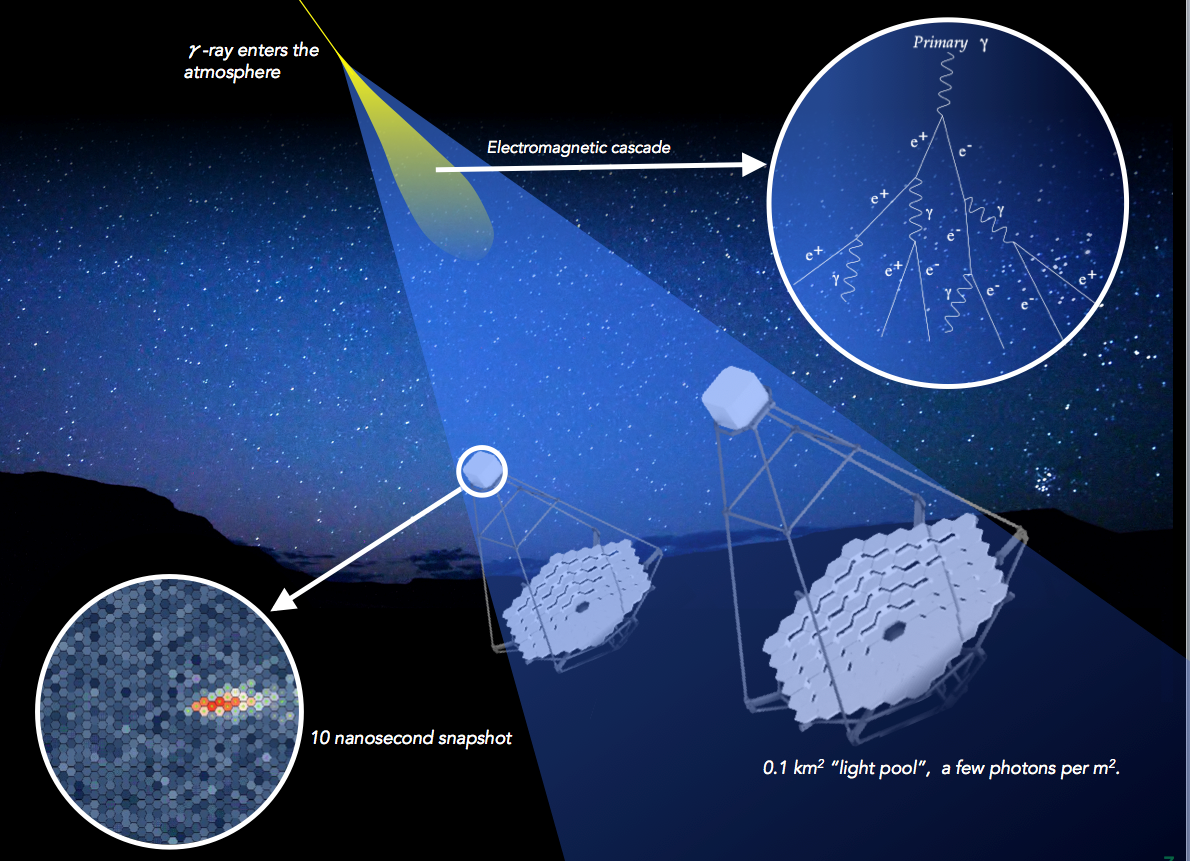
\includegraphics[width=1\textwidth]{figures/introduction/cherenkov-imaging.png}
\caption{Image explaining how Cherenkov Telescopes detect Cherenkov light produced by a primary $\gamma$-ray interacting with the Earth’s atmosphere. Credits to \cite{ctaobservatorywebsite}.}
\label{f:cherenkov-imaging}
\end{figure}
Electromagnetic showers, like those initiated by gamma rays, are different from hadronic showers initiated by Cosmic Rays (protons and nuclei) that have larger structures and can therefore be distinguished. The air showers initiated by electrons/positrons constitute an irreducible isotropic background for the telescopes. The efficiency in discriminating between hadronic and $\gamma$-ray showers defines, among other parameters, the telescope's minimum detectable flux or sensitivity \cite{tampieri2020real}. After the raw data is collected, an image-cleaning process occurs to reconstruct the shower information needed to perform the parametrization of the shower itself. A. M. Hillas introduced the fundamental image parameters in 1985 when a single telescope configuration was still used \cite{hillas1985cerenkov}. These parameters are:
\begin{itemize}
    \item Size: total number of photoelectrons in the shower image. It is proportional to the energy of the incoming primary $\gamma$-ray or particle;
    \item Length: is the half of the major axis of the shower image;
    \item Width: is the half of the minor axis of the shower image;
    \item Frac: measures the general concentration of light;
    \item Miss: is the perpendicular distance of the center of the field (where the source is supposed to be in a single telescope configuration and pointing in center of the field of view) from the image axis;
    \item Azimuthal-Width: is the image width relative to a new axis which
joins the center of the field to the centroid of the image; 
    \item Distance: is the distance of the brightest point from the center of the
field.
\end{itemize}
These parameters allow for evaluating the obtained Cherenkov images and achieving good $\gamma$-ray/hadron separation. 
New parameters are used to track the source position when the source is not in the camera center (see \autoref{ss:pointing-modes}):
\begin{itemize}
    \item Alpha: is the angle between the major axis of the ellipse and the direction of the source position from the center of gravity of the image;
    \item Dist: is the distance of the center of gravity of the image from the source position.
\end{itemize}
\begin{figure}[ht] 
\centering
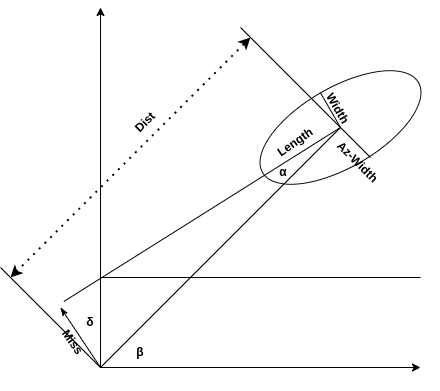
\includegraphics[width=0.7\textwidth]{figures/introduction/hillas.png}
\caption{Parametrization of a shower image through Hillas parameters.}
\label{f:hillas}
\end{figure}
\autoref{f:hillas} shows the Hillas parametrization of a shower image.
As we will see in \autoref{ss:telescope-array}, the Cherenkov Telescope Array Observatory will use an array of Cherenkov telescopes to observe individual showers to reconstruct the three-dimensional origin of $\gamma$-ray showers. This technique, known as stereoscopic reconstruction, allows more effective reconstruction and discrimination of $\gamma$-ray showers from hadronic showers produced by isotropic cosmic rays. The stereo reconstruction increases the background suppression efficiency by about 100, improves the angular resolution, and enables morphological studies of extended $\gamma$-ray sources \cite{Spurio2018}.
These observations are analyzed using reconstruction algorithms based on Hillas’ parameters and implemented using statistical techniques like the Random Forest regression method \cite{Albert2008}. After the data is reconstructed, it is collected in the form of a photons list, i.e., a collection of individual photons along with their arrival time, reconstructed direction, and reconstructed energy. 



\section{The Cherenkov Telescope Array Observatory}
\label{s:CTA}
The Cherenkov Telescope Array (CTA) Observatory is a next-generation ground-based $\gamma$-ray observatory currently under development. CTA is a collaboration of over 1200 scientists from 32 countries and is expected to be the most sensitive and highest-resolution $\gamma$-ray observatory ever built \cite{ScienceWithCherenkovTelescopeArray2018}.

\subsection{Science goals}
\label{s:science-goals}
CTA will address a wide range of major questions in and beyond astrophysics. The Core Programme \cite{ScienceWithCherenkovTelescopeArray2018} provides a comprehensive discussion. In brief, the science goals can be grouped into three broad themes. 

The first theme is understanding the origin and role of relativistic cosmic particles. Relativistic particles play a significant role in many astrophysical systems, from pulsars and supernova remnants to active galactic nuclei and clusters of galaxies. However, the relationship between these particles, the turbulent motions of gas, and magnetic fields within our own galaxy and their overall impact on star formation and galaxy evolution is not well understood. CTA will provide the first high-resolution measurements of cosmic-ray protons and nuclei in astrophysical systems, giving insight into the processes of acceleration, transport, and feedback mechanisms. Historically, non-thermal effects in astrophysical systems have been ignored or approximated due to a lack of data. The insights from CTA will significantly contribute to our understanding of galaxy and cluster evolution in the era of precision astrophysics. The main goal of $\gamma$-ray astrophysics has been to identify where particle acceleration occurs and determine the main contributors to locally measured cosmic rays, mostly protons, and nuclei. Progress has been made in the last decade. Still, key questions remain unanswered, such as whether supernova remnants are the only major contributors to Galactic cosmic rays and the sources of high-energy cosmic electrons and ultra-high-energy cosmic rays. The question of how and where particles are accelerated in the universe is also important, as well as the role these particles play in the evolution of their host objects and how they are transported to large distances.

The second theme is about probing extreme environments. The acceleration of particles to extremely high energies is often linked to extreme environments, such as those found near neutron stars and black holes or in relativistic outflows or explosions. Very high-energy (VHE) emissions from these accelerated particles can serve as a probe of these environments, providing access to time and distance scales that are not accessible through other wavebands. VHE emission also often escapes from systems where UV and X-ray emission is absorbed, offering information independent of assumptions about magnetic field strengths. Furthermore, VHE photons from distant objects can probe the intervening space. CTA will allow us to measure the redshift evolution of the UV-IR background and, thus, the star-formation history of the universe and probe magnetic fields in cosmic voids at levels many orders of magnitude below the reach of any other technique. CTA will also determine if VHE photons heat the gas in these under-dense regions, potentially suppressing the formation of dwarf satellite galaxies.

The third theme is exploring frontiers in physics. CTA has the potential to make significant discoveries in the field of fundamental physics. CTA will reach the expected thermal relic cross-section for self-annihilating dark matter for a wide range of dark matter masses, including those inaccessible to the Large Hadron Collider. The long travel times of gamma rays from extragalactic sources, combined with their short wavelength, make them a sensitive probe for energy-dependent variations of the speed of light due to quantum-gravity-induced fluctuations of the metric. CTA will be sensitive to these effects on the expected characteristic scale, the Planck scale. Gamma rays may also couple to other light particles, such as axion-like particles (ALPs), under the influence of intergalactic magnetic fields, which effectively makes the universe more transparent to gamma rays and introduces a spectral modulation. Each of these effects would represent a major discovery and justify the effort of constructing and operating CTA. CTA's increased sensitivity and energy coverage bring these effects within reach and could allow for further discoveries in fundamental physics.


\subsection{The telescope array}
\label{ss:telescope-array}
CTA aims to capture the elusive cascades of $\gamma$-ray photons produced when high-energy gamma rays hit the Earth's atmosphere. These cascades are incredibly rare, with only one $\gamma$-ray photon per square meter per year from a bright source or one per square meter per century from a faint source. CTA will use more than 60 telescopes distributed between two array sites in the northern and southern hemispheres to improve the chances of capturing these elusive signals. The northern hemisphere array will have a more limited size and focus on the low and mid-energy range of CTA, between 20 GeV and 5 TeV. Meanwhile, the southern hemisphere array, which has a prime view of the rich central region of our galaxy, will cover the mid- to a high-energy range of CTA, spanning $\gamma$-ray energies from 150 GeV to 300 TeV \cite{Acharyya201935}. \autoref{fig:cta-sens} shows the sensitivity of the northern and southern telescope arrays compared to other instruments. 
\begin{figure}[]
\centering
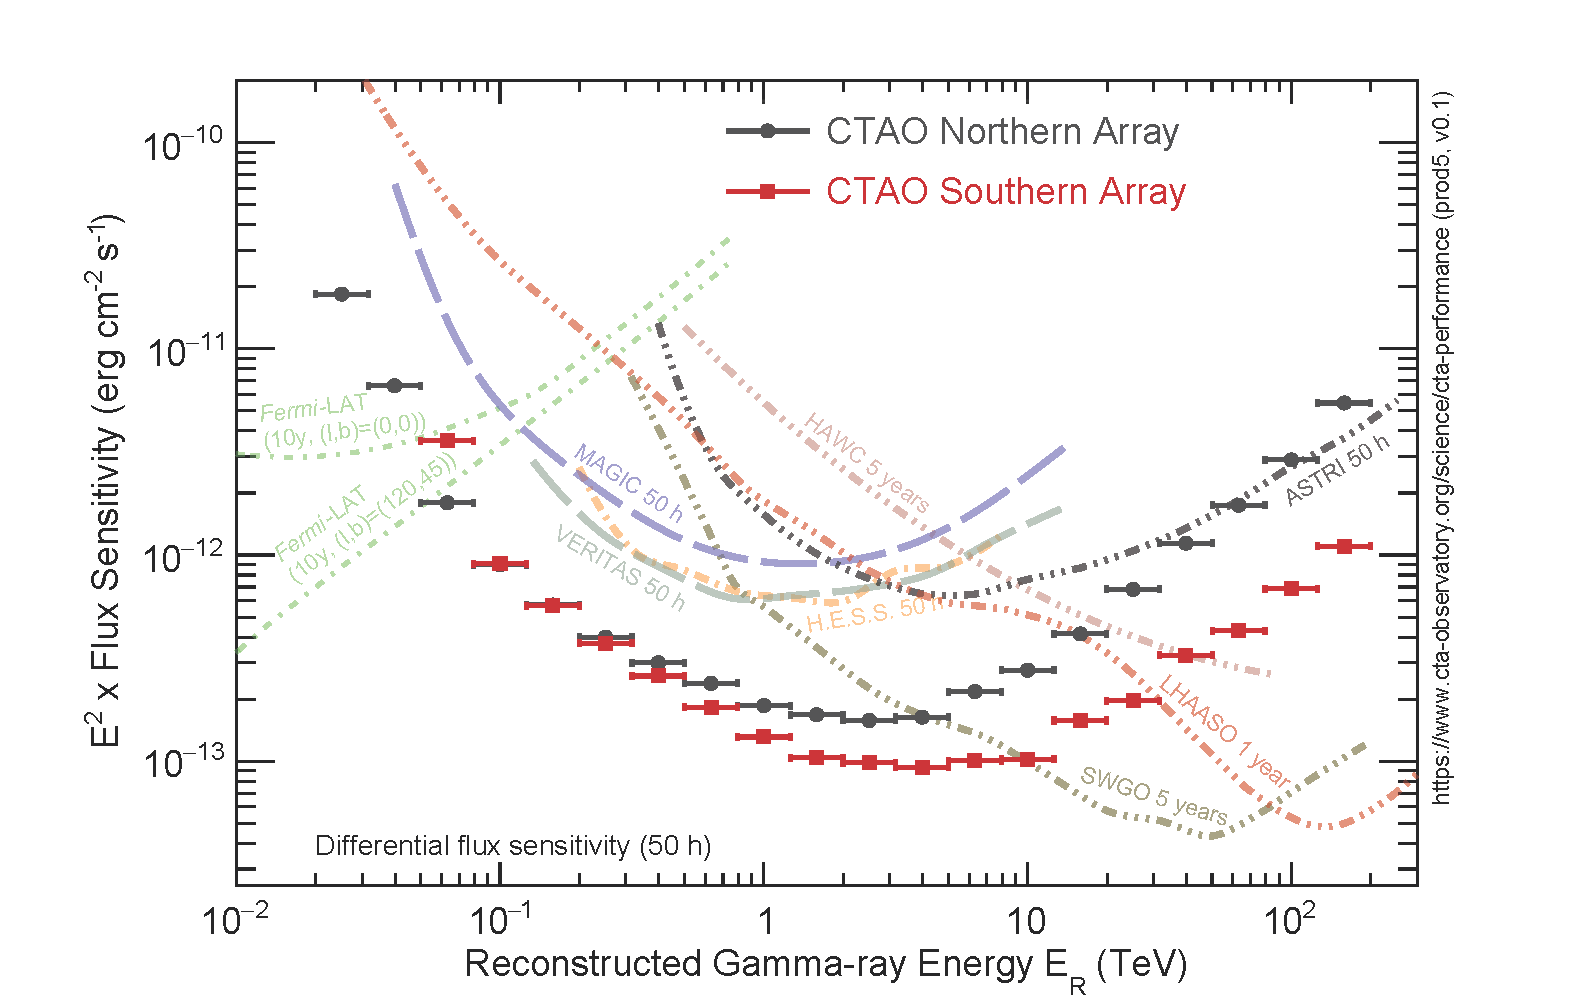
\includegraphics[width=1\linewidth]{figures/introduction/ctao-sensitivity.png}
\captionof{figure}{The sensitivity of the CTA Northern and Southern arrays compared to other instruments. Credits to \cite{zenodo_2021}}
\label{fig:ctao-sens}
\end{figure}
To cover the full CTA energy range, three classes of telescopes are required: Small-Sized Telescope (SST), Medium-Sized Telescope (MST), and Large-Sized Telescope (LST). The SSTs are the most sensitive to detect high-energy gamma rays and are therefore more suitable for the southern site's detection of higher-energy gamma rays. The MSTs and LSTs will be installed in both array sites. Scientists have conducted various simulations to determine the best configurations of arrays to maximize performance, including sub-array configurations. These configurations (shown in \autoref{fig:ctao-north} and \autoref{fig:ctao-south}) could allow for parallel and independent observations, resulting in optimized observation time and a more specific focus on science \cite{Acharyya201935}. The Alpha Configuration is the approved layout of the telescope arrays in both the northern and southern hemispheres. This configuration includes 13 telescopes, 4 LSTs, and 9 MSTs, distributed over an area of about $0.5 km^2$ in the CTA Northern Array and 51 telescopes over a $~3 km^2$ area, consisting of 14 MSTs and 37 SSTs, in the CTA Southern Array. The collaboration between the northern and southern hemispheres will allow CTA to expand its reach and study the universe in a more comprehensive way \cite{Acharyya201935}. 
\begin{figure}[ht]
\centering
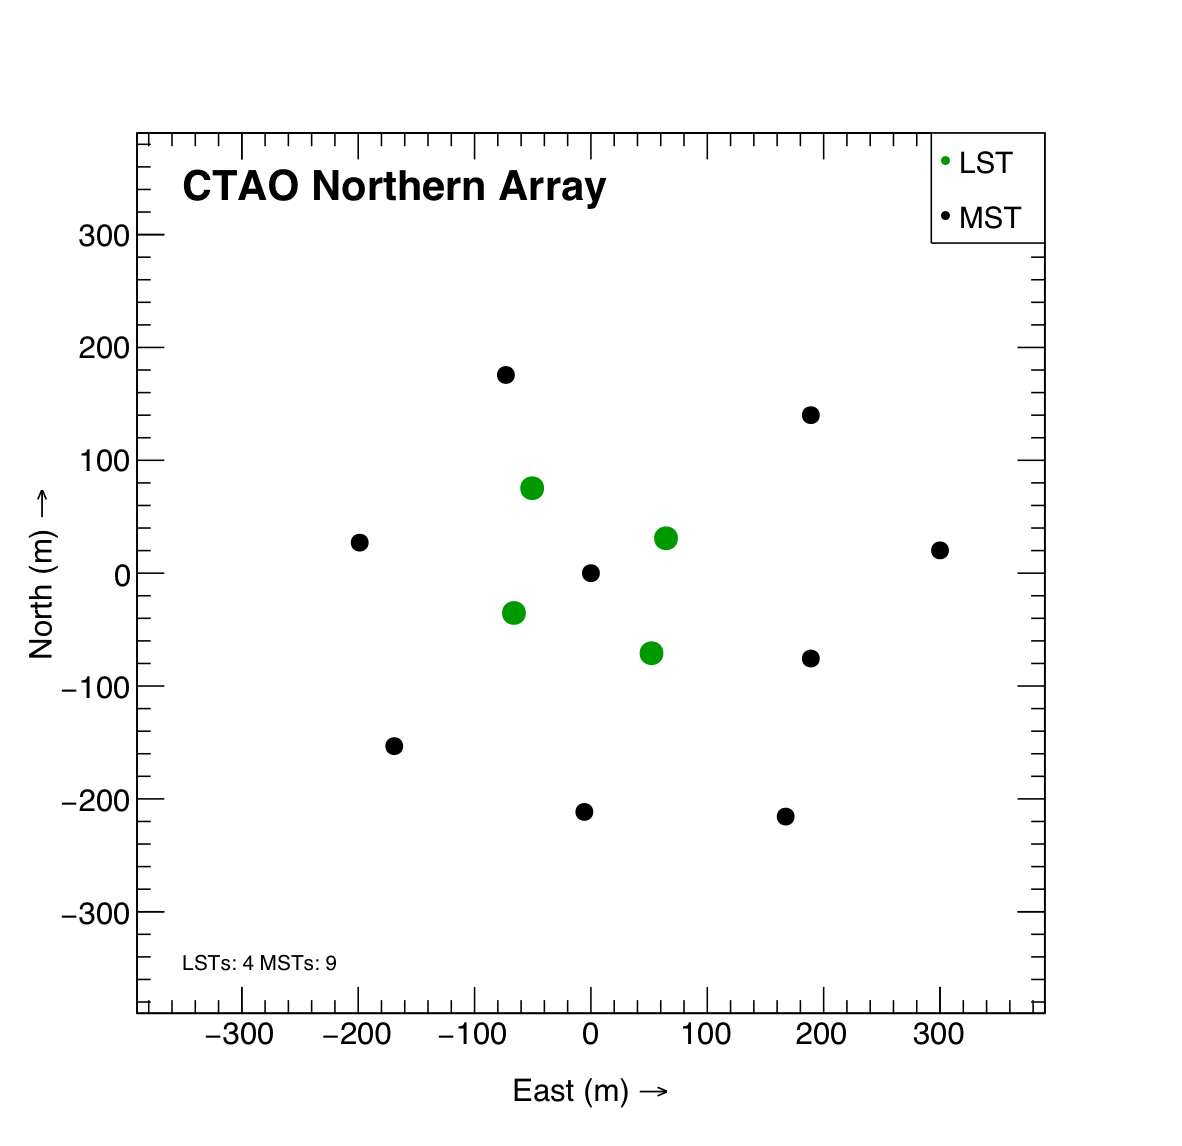
\includegraphics[width=0.8\linewidth]{figures/introduction/ctao-north.png}
\captionof{figure}{Layout of the CTA Northern array on La Palma (Spain), including the elements defined in the Alpha Configuration. Credits to \cite{zenodo_2021}}
\label{fig:ctao-north}
\end{figure}
\begin{figure}[ht]
\centering
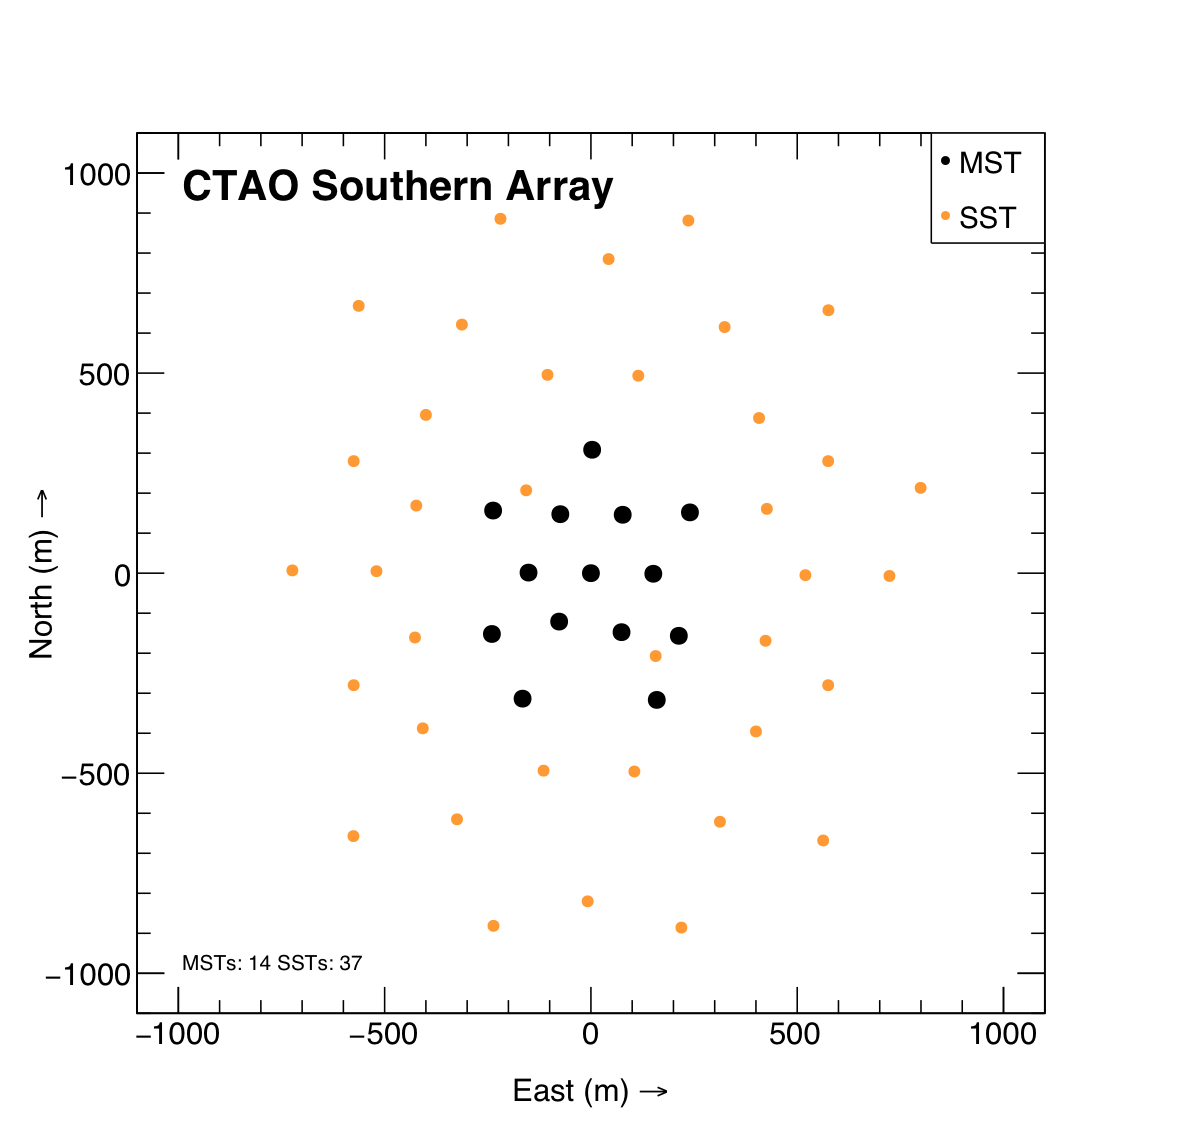
\includegraphics[width=0.8\linewidth]{figures/introduction/ctao-south.png}
\caption{Layout of the CTA Southern array in the Atacama Desert (Chile), according to the Alpha Configuration. Credits to \cite{zenodo_2021}}
\label{fig:ctao-south}
\end{figure}
The northern hemisphere array will be located at the existing site of the Instituto de Astrofisica de Canarias' (IAC's) Observatorio del Roque de Los Muchachos on the island of La Palma in the Canary Islands. This site already hosts an operating $\gamma$-ray observatory, the Major Atmospheric Gamma Ray Imaging Cherenkov (MAGIC) telescopes, and various optical telescopes of various sizes. The Southern Hemisphere Array will be located in the Atacama Desert in Chile, near the European Southern Observatory's (ESO's) existing Paranal Observatory. 

\subsubsection{Large-Sized Telescopes (LST)}
\begin{figure}[t]
\centering
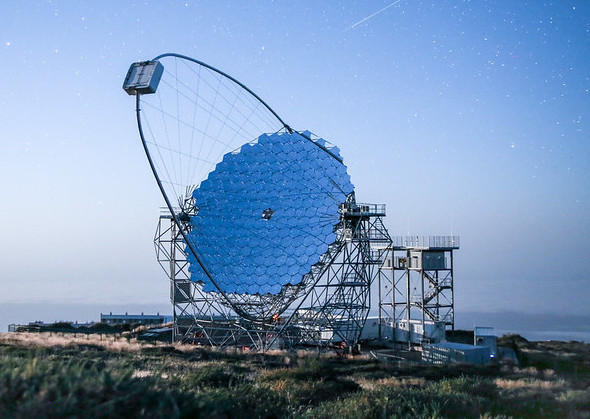
\includegraphics[width=0.9\linewidth]{figures/introduction/lst.jpg}
\caption{The LST Prototype, LST-1, on the CTA-North site in La Palma. Credits to \url{https://www.flickr.com/photos/cta_observatory/albums/72157671493684827}} 
\label{fig:lst}
\end{figure}
The Large-Sized Telescope (LST) project is a collaboration involving over 100 scientists from 10 countries, including Brazil, Croatia, France, Germany, India, Italy, Japan, Poland, Spain, and Sweden. The LST is designed to capture images of low-energy gamma rays, which produce a small amount of Cherenkov light. The LST uses a large mirror with a 23m diameter parabolic reflective surface supported by a tubular structure made of reinforced carbon fiber and steel tubes (\autoref{fig:lst}).  Four LSTs will be placed at the center of the northern hemisphere array to capture low energy sensitivity of CTA between 20 and 150 GeV. The LSTs also have a very good sensitivity up to energies of a few TeV, which is, however, more efficiently covered by Medium-Sized Telescopes (MSTs). The LST is an alt-azimuth telescope that uses a reflective surface of $400 m^2$ to collect and focus the Cherenkov light into the camera. The camera comprises photomultiplier tubes that convert the light into electrical signals that dedicated electronics can process. Although the LST is 45m tall and weighs around 100 tonnes, it is designed to be extremely nimble and able to re-position within 20 seconds. This re-positioning speed and low energy threshold are critical for CTA studies of galactic transients, high red-shift active galactic nuclei, and $\gamma$-ray bursts. The LSTs will also expand the science reach to cosmological distances and fainter sources with soft energy spectra. 
The LST Camera shares many elements with the NectarCAM for the MSTs. The camera has a total field of view of about 4.3 degrees and is designed to be compact and lightweight while providing optimal performance at low energies. Each pixel incorporates a photosensor and the corresponding readout electronics. These electronics are based on the Domino Ring Sampler Version 4 (DRS4) chip, developed at the Paul Scherrer Institute in Switzerland and currently used by several experiments; among them the MAGIC Cherenkov telescopes. The camera trigger strategy is based on the shower topology and the temporal evolution of the Cherenkov signal produced in the camera. The LST prototype, LST-1, was completed in October 2018 in La Palma, Canary Islands, Spain, on the site of the Observatorio del Roque de Los Muchachos. The prototype is foreseen to become the first LST telescope of CTA and, in fact, the first telescope on a CTA site to be operated by the observatory. It will need to undergo a critical design review to verify that the design complies with CTA science goals, operational needs, safety standards, etc. before CTA formally accepts it.
On October 10th, 2018, over 200 guests from around the world gathered to celebrate the inauguration of the prototype Large-Sized Telescope (LST-1). On December 14th, 2018, the LST-1 prototype recorded its first Cherenkov light. On November 23rd, 2019, LST-1 successfully detected its first $\gamma$-ray signal when pointing to the Crab Nebula. Between January and February 2020, the LST-1 prototype observed the Crab Pulsar, a neutron star at the center of the Crab Nebula. These observations were used to verify the telescope's performance and capabilities.

\subsubsection{Medium-Sized Telescopes (MST)}
\begin{figure}[t]
\centering
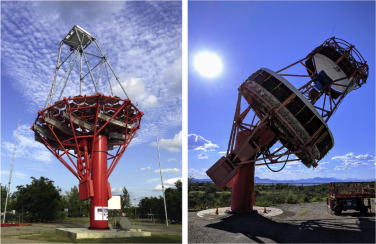
\includegraphics[width=0.9\linewidth]{figures/introduction/mst.jpg}
\caption{The MST design explores two different concepts. On the one hand, inspired by HESS and VERITAS current observatories, a 12 meters diameter modified Davis–Cotton (DC-MST) optical layout and a PMT camera. On the other, a novel 10 meters diameter Schwarzschild–Couder (SC-MST) optics incorporating a novel Silicon Photo-Multiplier (SiPM) camera. Credits to \cite{Barrio_2020}.} 
\label{fig:mst}
\end{figure}
An international team of institutes and universities from Austria, Germany, France, Brazil, Poland, Spain, Switzerland, and Italy is developing the Medium-Sized Telescope (MST). This telescope is considered the \textit{workhorse} of the Cherenkov Telescope Array (CTA), with sensitivity in the core energy range of CTA, from about 150 GeV to 5 TeV. The CTA plans to include 23 MSTs, with 14 in the southern and 9 in the northern hemispheres. The MST mirror will be about 12 meters in diameter and have two camera designs using photomultiplier tubes (PMTs).
The MST is a modified Davies-Cotton telescope with a reflector diameter of 12 meters on a polar mount and a focal length of 16 meters. To create a uniform reflector, the MST will have up to 90 hexagonal-shaped mirrors aligned with an active mirror control assembly. The MST cameras will have a large field of view of about 8 degrees, making it easier to observe $\gamma$-ray sources that may be concentrated in one area of the sky or widely spread apart. Two camera concepts are in development for the MST: NectarCAM and FlashCAM. NectarCAM uses the ‘Nectar’ analog pipeline ASIC for signal capture with GSample/s sampling rate and shares many design features/components with the LST camera. NectarCAM is composed of 265 individual and easily removable modules. FlashCAM design follows a horizontal architecture with the photon detector plane (PDP), the readout electronics (ROS), and the data acquisition system (DAQ) as key building blocks. The PDP contains photomultiplier tubes (PMTs) arranged in a hexagonal structure.
An MST prototype was deployed in Berlin in 2012 and is currently undergoing performance testing. The main purpose of the prototype is to validate the design of the individual components, test the interfaces between the mating assemblies, and define the assembly process of the product. The prototype has a fully functional drive system, cameras for pointing and tracking, sensors designed to record the behavior response of the structure and drive system, and a weather station. The prototype is a fully-functioning telescope but doesn't include the entire camera assembly and its readout. Camera demonstrators were built, tested, and validated in parallel by the two camera sub-projects.

\subsubsection{Small-Sized Telescopes (SST)}
\begin{figure}[t]
\centering
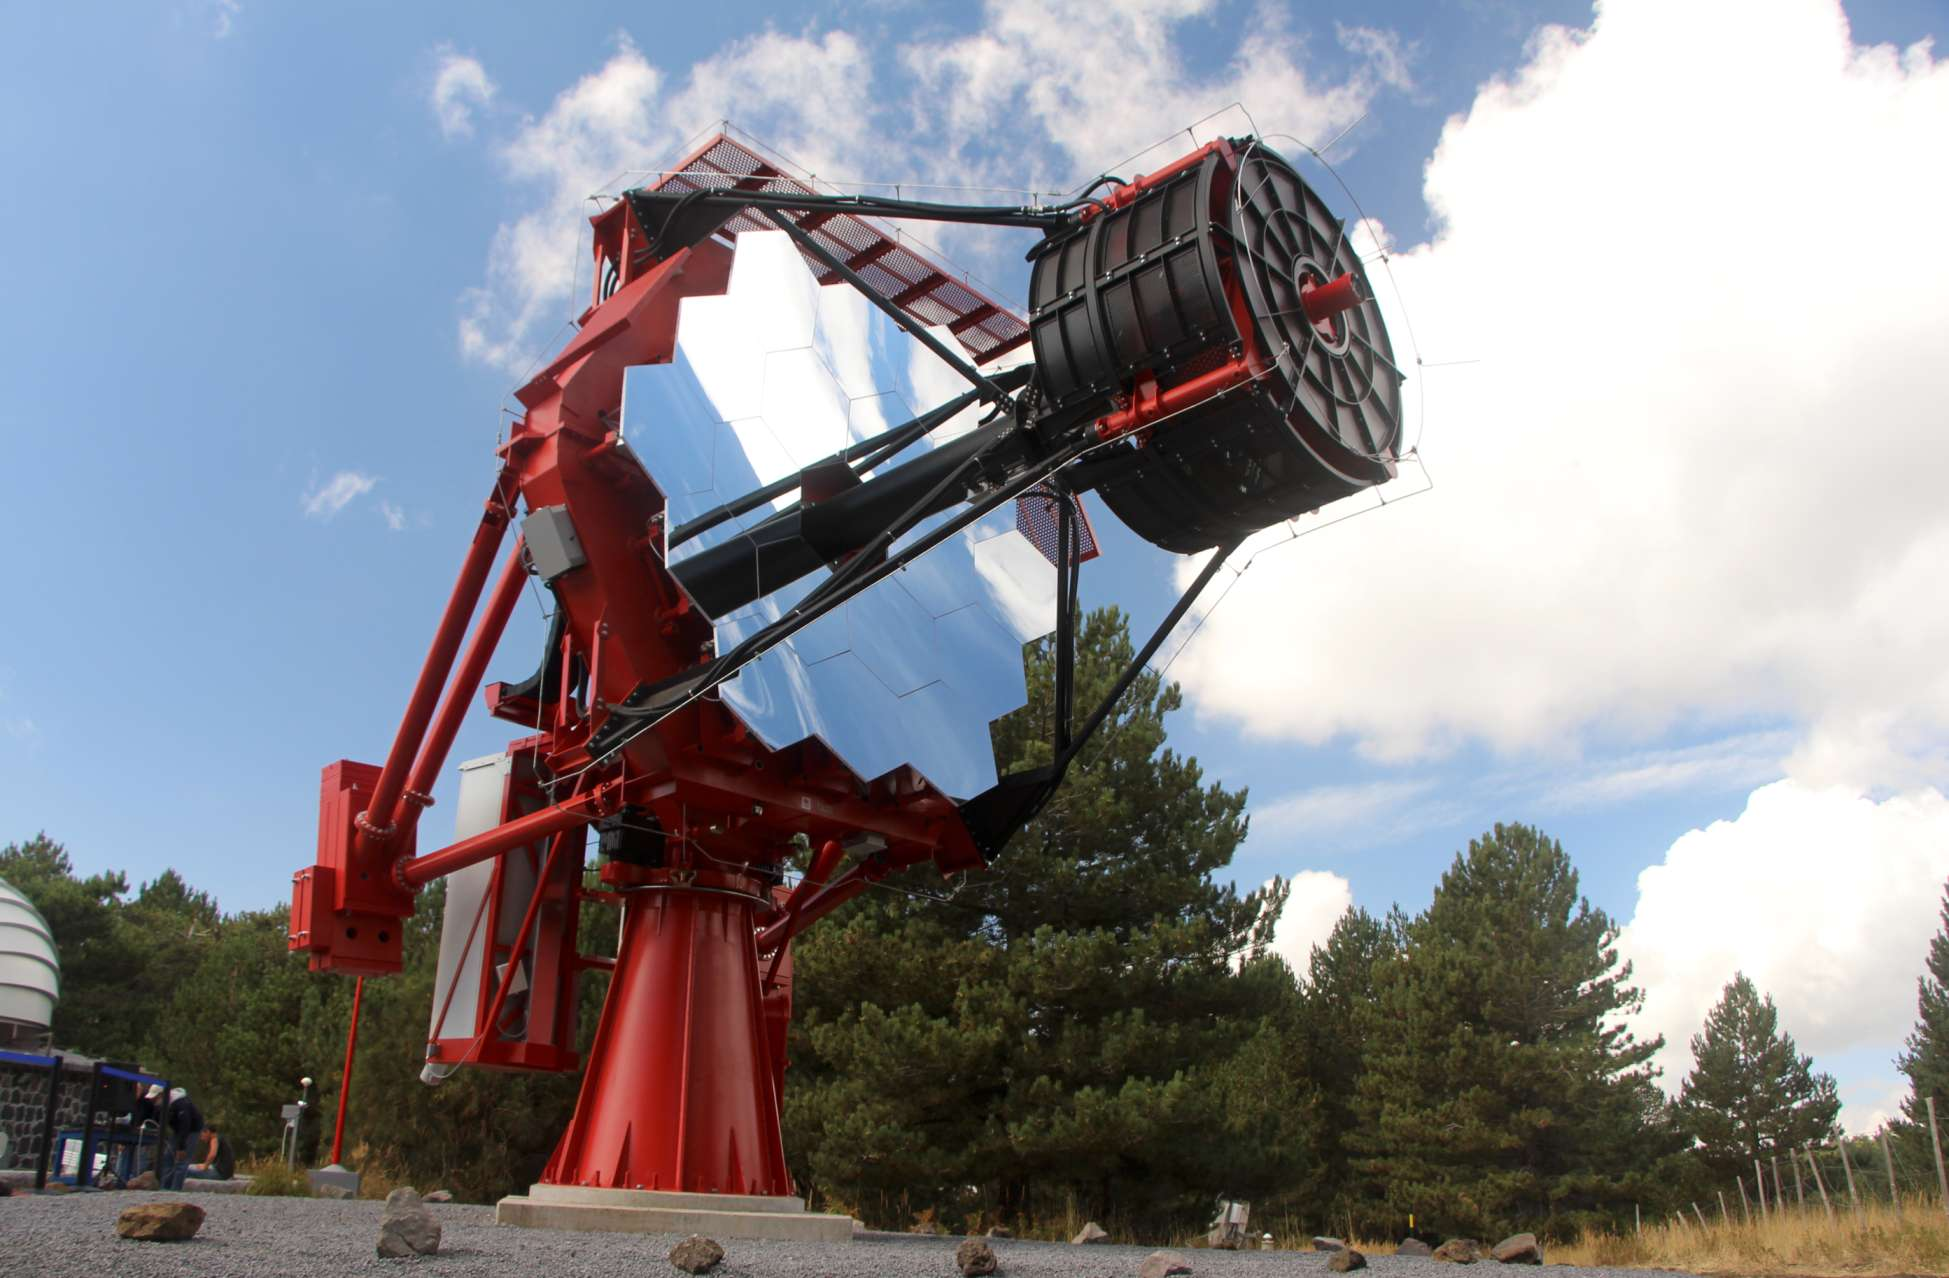
\includegraphics[width=0.9\linewidth]{figures/introduction/sst.jpg}
\caption{The ASTRI telescope prototype, a novel dual-mirror Schwarzschild-Couder telescope design proposed for the Cherenkov Telescope Array (CTA). Credits to \cite{ctaobservatorywebsite}} 
\label{fig:sst}
\end{figure}
The Small-Sized Telescopes (SSTs) will make up the largest number of telescopes in the Cherenkov Telescope Array (CTA), with 37 planned to be spread out over several square kilometers in the southern hemisphere array only. This is because very high-energy $\gamma$-ray showers produce a large amount of Cherenkov light over a large area. The SST's smaller mirror is sensitive to the highest energy gamma rays (between a few TeV and 300 TeV). The SSTs wide coverage and high sensitivity improve CTA's chances of detecting the highest energy gamma rays. Three different SST implementations were proposed for the final SST design: ASTRI-Horn, GCT, and SST-1M. In 2018, a harmonization process was initiated. In June 2019, the council accepted the CTA Management proposal, stating that \textit{the CTA-SST design should be based on the ASTRI/CHEC design, taking into account the experience gained from all designs}. The SST design is a dual-mirror Schwarzschild-Couder aplanatic configuration, and thanks to its small plate scale, it uses a novel compact camera based on SiPM sensors. The 4.3m diameter primary mirror is segmented into hexagonal facets, and the 1.8m secondary mirror is monolithic. The SST's camera, also known as the CHEC camera, uses custom peak-hold application-specific integrated circuits (ASICs) for signal capture. The dual-mirror design allows for the same angular resolution and collecting area across a wide field of view with a short focal length. The camera comprises 2048 silicon photo-multiplier pixels forming approximately a 9x9 degrees field of view. The CHEC is unique as an SST dual-mirror camera in its ability to capture Cherenkov light not as fixed images but as movies consisting of hundreds of frames, each lasting one billionth of a second. The SST collaboration benefits from the research and development work previously carried out within the ASTRI, CHEC, and GCT projects to develop end-to-end SST dual-mirror telescopes. The ASTRI project is led by the Italian National Institute of Astrophysics (INAF) with the collaboration of several Italian universities, the Italian National Institute of Nuclear Physics (INFN), Universidade de São Paulo in Brazil, and North-West University in South Africa. The CHEC project, led by MPIK, is an international collaboration between the University of Adelaide, the University of Amsterdam, DESY Zeuthen, Durham University, the Erlangen Centre for Astroparticle Physics (ECAP), the University of Leicester, the University of Liverpool, Nagoya University, and the University of Oxford. The Observatoire de Paris-Meudon carries out the GCT telescope project.

\subsection{Computing and software}
The CTA Computing Department faces the challenge of designing and implementing a system that supports all aspects of the CTA Observatory, from accepting observation proposals to scheduling observations, controlling the telescopes, processing and archiving data, and making it accessible to the public using open standards and FAIR (findability, accessibility, interoperability, and reusability) principles. The department is responsible for all stages of development, from architectural design to construction, validation, deployment, and maintenance. The Observatory's technical challenges and long lifetime will require new techniques and technologies to meet scientific demands. Even when built, maintaining the software and hardware systems for the 30-year lifespan of the Observatory, and the science data archive for an additional 10 years, will not be a simple task. Therefore, software systems engineering is just as crucial as the code itself. In addition, the CTA array sites will generate a vast amount of data from the telescopes in hundreds of petabytes annually. This data will then be compressed and reduced to a few petabytes per year before being transferred to off-site data centers for processing and storage. Additionally, tens of petabytes of simulated data will also be generated and processed.
\begin{figure}[ht]
\centering
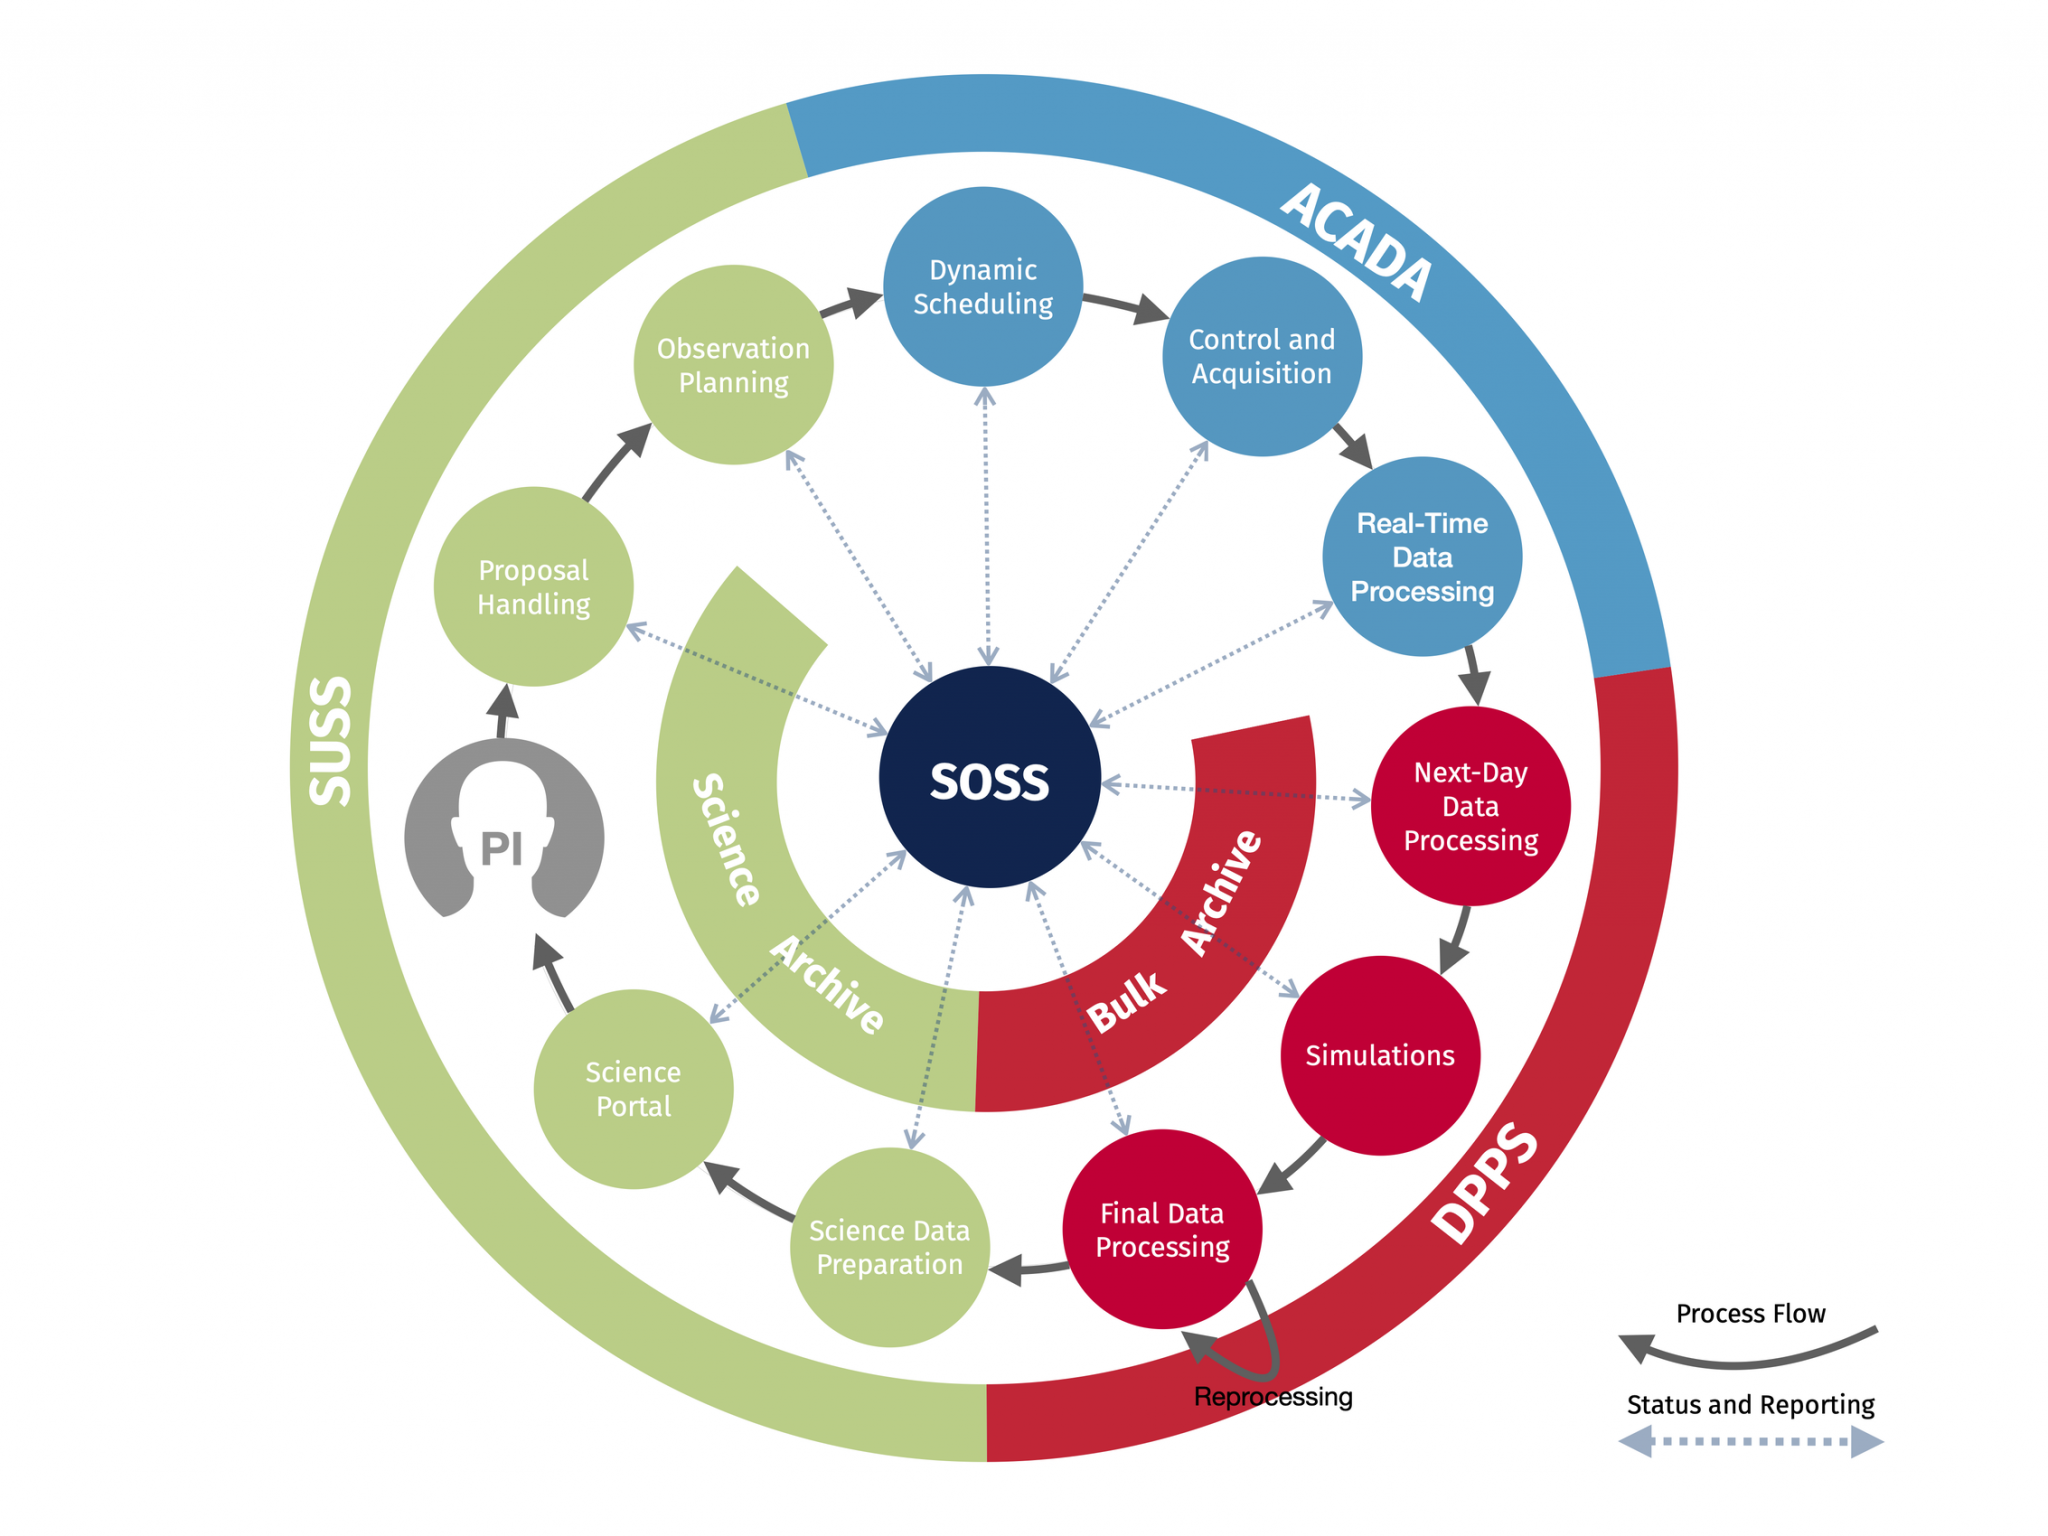
\includegraphics[width=0.9\linewidth]{figures/introduction/cta-softwares.png}
\caption{The diagram below provides a general overview of how the software systems interact with the main processes involved in the science operations of the observatory, including the submission, execution, and return of processed data related to a scientific proposal. Credits to \cite{ctaobservatorywebsite}}
\label{fig:cta-softwares}
\end{figure}
The software systems that will satisfy all the CTA requirements are shown in \autoref{fig:cta-softwares}: the Array Control and Data Acquisition System (ACADA), the Data Processing and Preservation System (DPPS), the Science User Support System (SUSS), and the Science Operations Support System (SOSS). 
The ACADA (Acquisition and Control and Data Analysis) system manages the supervision and control of telescopes and calibration instruments at both CTA array sites, including the efficient execution of scheduled and dynamically triggered observations. It also manages raw data acquisition and compression and generates automatic science alerts. The ACADA provides a user interface for site operators and astronomers \cite{Oya2017}. It's composed of several subsystems such as the Resource Manager and Central Control system \cite{Melkumyan2019}, the Human Machine Interface system \cite{Sadeh2017}, the Short-Term Scheduler system \cite{Colome2014}, and the Science Alert Generation Pipeline \cite{Bulgarelli2014}. The latter allows the observatory to reconstruct and analyze the data, detect sources, and issue candidate science alerts in real time. As we will see later, this system is the context in which this work has been carried out. The DPPS (Data Processing and Preservation System) is responsible for transforming the raw data products generated by ACADA into low-level science data products suitable for analysis, which are then delivered to the SUSS (Science User Support System) for dissemination. The DPPS ensures that all data products are preserved and replicated in at least two off-site data centers, have traceable and reproducible provenance, and are of the highest scientific quality. It also provides continuous monitoring and quality reporting for its sub-systems and produces high-level science quality metrics and reports related to the services provided. The DPPS is implemented as a distributed system, deployed as a set of Data Processing and Preservation Nodes, running at the CTA-North and CTA-South data centers, on three CTA off-site data centers, and at the SDMC Data Center \cite{ctaobservatorywebsite}. The SUSS manages the software system for high-level science operations workflows, from proposals to data delivery and user support. It is the main access point for exchanging science-related products with science users. It provides software for observation planning, the automatic generation and verification of high-level science data products, the Science Archive, Science Analysis Tools, and Science Portal, which provides access to software applications, services, data, and software products \cite{Oya2017}. The SOSS (Science Operations Support System) is a collection of software tools that support the systems involved in science operations workflows, such as ACADA, DPPS, and SUSS \cite{ctaobservatorywebsite}. The respective systems can access and share science operations-related information and configurations. It includes the means to track the state of proposals and observations throughout their life cycle and the state of the CTA Observatory throughout the science operations workflow and science performance.


\subsection{The Science Alert Generation System}
\label{s:sag}
As stated in the section above, the Science Alert Generation system will perform real-time scientific analysis to issue science alerts. A science alert is a notification within the astrophysics community to share information about a transient phenomenon (such as an AGN's $\gamma$-ray flare, $\gamma$-ray bursts, gravitational waves, or galactic transients) that has been observed. Sharing this information through specialized communication networks allows coordination among different observatories to enable multi-wavelength and multi-messenger analysis. Those are rapidly developing fields that study celestial objects and phenomena using a wide range of electromagnetic and non-electromagnetic signal. This includes everything from radio waves and visible light to gamma rays, gravitational waves and particles, such as cosmic rays and neutrinos. One of the key advantages of multi-wavelength and multi-messenger astronomy is that it allows astronomers to study the universe from a more comprehensive and holistic perspective. By combining data from different wavelengths and messengers, astronomers can better understand the physical processes in the universe. One of the most significant developments in multi-wavelength and multi-messenger astronomy has been detecting gravitational waves, ripples in space-time predicted by Einstein's theory of general relativity. The acceleration of massive objects, such as the merging of binary black holes or neutron stars, produces these waves. The first gravitational wave detection was made in 2015 by the Laser Interferometer Gravitational-Wave Observatory (LIGO) \cite{gw_061102}. Since then, several other gravitational wave detections have been made, opening up a new window onto the universe \cite{abbott2016observation}. The Science Alert Generation system will have a key role in the GW follow-up program \cite{seglar2019gravitational}. Another important aspect of multi-wavelength and multi-messenger astronomy is the study of transient phenomena, such as supernovae, $\gamma$-ray bursts, and fast radio bursts. These events are often brief and elusive and can be studied more effectively by combining data from multiple telescopes and instruments. For example, the combination of data from X-ray, optical, and radio telescopes has allowed for the study of the afterglows of $\gamma$-ray bursts (GRBs), which are thought to be the result of the collapse of massive stars or the merging of binary neutron stars \cite{Fishman1995}.
To achieve collaboration between observatories, the transient phenomena must be observed in real-time on a short timescale. Furthermore, suppose other observatories identify a transient. In that case, it is important to react quickly, repoint the telescopes, and analyze the data in an automated and fast way to confirm the transient event and to conduct follow-up observations \cite{Bulgarelli_2021}. 
\subsubsection{Requirements}
\label{ss:sag-requirements}
Technical challenges, such as limited network bandwidth at the observatory sites and a high expected data rate, make it difficult to perform real-time analysis off-site. As a result, an on-site analysis pipeline is necessary to access raw data, perform calibration, and produce scientific results \cite{bulgarelli2015on}. The real-time analysis must meet challenging requirements to process the large amount of data produced by CTA in real-time. The Science Alert Generation system must be able to generate candidate science alerts within 20 seconds from the last acquired event, with a maximum telescope positioning time of 90 seconds in response to external or internal triggers. These candidate science alerts will be sent to the Transients Handler system, which will evaluate the results of the SAG to generate the final science alert to the community within 5 seconds of receiving it. If we also consider the 5 seconds required to acquire data, CTA will be capable of issuing science alerts with a maximum latency of 30 seconds \cite{Bulgarelli_2021}.
Furthermore, the SAG system must be available during observations for at least 95\% of the time to enable real-time follow-up of external alerts and internal alerts triggering serendipitous discoveries. This will require re-scheduling observations to follow up the phenomena in real-time and maximize the coordinated outcome of the facilities' network \cite{di2020detection}. According to the CTA design requirements, the real-time search for transient events should be performed on multiple time scales (from minutes to hours) with a sensitivity not worse than two times the nominal CTA sensitivity. The sensitivity is defined as the minumum flux value detectable with a confidence level of $5\sigma$ and it depends on several parameters, such as the analysis algorithm, the observing conditions, the instrument response function, and the sub-array configuration.
\cite{fioretti2015real} performed a preliminary evaluation of the real-time analysis sensitivity as a function of the CTA high-level technical performance (e.g., effective area, point spread function) and the observing time. 
 
\subsection{The scientific use cases}
\label{s:contribution-1-use-cases}
The growing interest in multi-messenger and multi-wavelength astronomy has greatly enhanced the search for transients. As stated in \autoref{s:science-goals}, the KSP for transients plans to invest a significant amount of observation time per year (\autoref{fig:transient-schedule}). The main source classes targeted by this KSP are Gamma-Ray Bursts (GRBs), Galactic transients, X-ray, optical, and radio transients, High-energy neutrino transients, GW transients, and serendipitous VHE transients \cite{ScienceWithCherenkovTelescopeArray2018}. GRBs are expected to be a major component of this KSP and will be detected based on external alerts (covered in \autoref{s:follow-up-observation}), but with the possibility of serendipitous discoveries (covered in \autoref{s:serendipitous-discoveries}).
\begin{figure}[t]
\centering
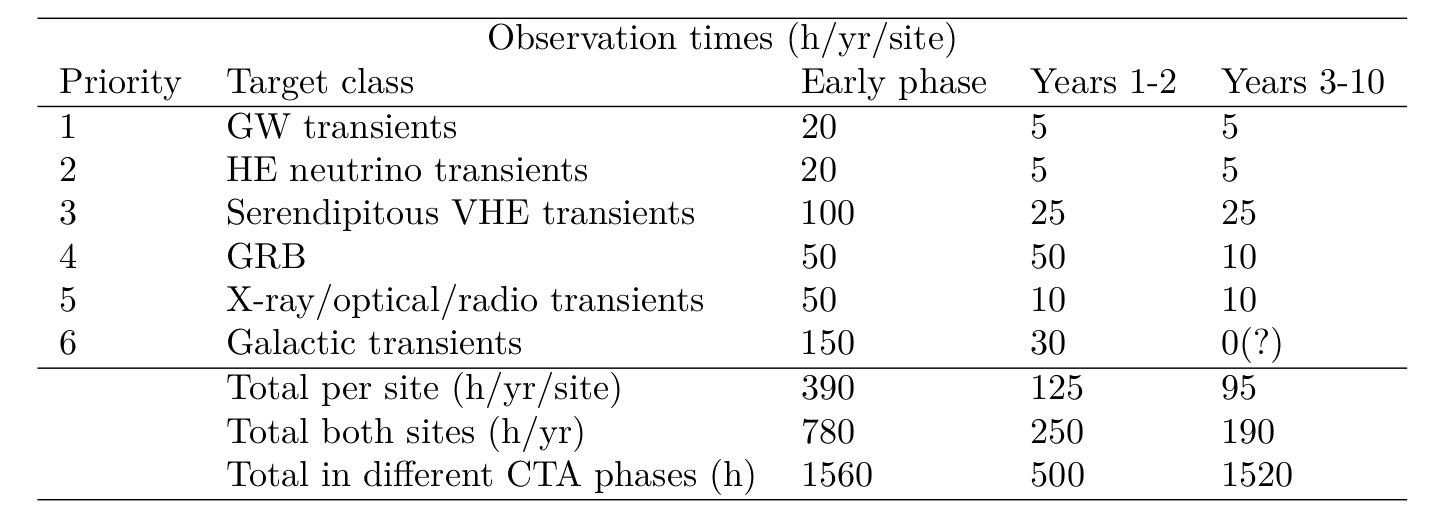
\includegraphics[width=0.9\linewidth]{figures/introduction/transients-schedule.png}
\caption{Maximum observation times required for follow-up targets in the Transient KSP, taken from. Credits to \cite{di2020detection}}
\label{fig:transient-schedule}
\end{figure}

\subsubsection{Serendipitous discoveries}
\label{s:serendipitous-discoveries}
Serendipitous discoveries are unexpected findings made while studying a specific target or phenomenon. This can happen because the telescope's field of view is larger than the region of interest used to observe a particular source. However, the probability of a serendipitous GRB event appearing in the field of view during an observation is very low. For example, when the observatory generates catalogs of known sources, it will cover large areas of the sky for a long time, increasing the probability of seeing a serendipitous event. The event must be detected as soon as possible to broadcast a science alert to other observatories to follow the same event and enable multi-wavelength and multi-messenger analysis. 

\subsubsection{Follow-up observation triggered by an external science alert}
\label{s:follow-up-observation}
Follow-up observations refer to a strategy of observing a specific target or phenomenon in more detail after an initial discovery or detection. The follow-up observations can be triggered by a science alert, which is a notification that alerts researchers and facilities of an interesting or unusual event happening. Follow-up observations can be conducted using various instruments and techniques. They are typically performed to study a target in more detail, confirm an initial discovery, and gather additional information about the target's properties \cite{ScienceWithCherenkovTelescopeArray2018}. When a science alert is received, the observatory will interrupt the current observation and will point to a new sky region to detect the new source in the least possible time. Suppose the error on the source's position is bigger than the field of view of the telescopes. In that case, multiple follow-up observations with a tiling strategy \cite{bulgarelli2015on} are required to cover the whole localization region. In addition, the event's evolution can not be observed from the beginning due to the delay between detecting the source that triggered the science alert and the time the telescopes took to change their pointing to the new sky region. 


\section{Gamma Ray Bursts}
\label{s:Gamma-Ray-Bursts}
\begin{figure}[t]
\centering
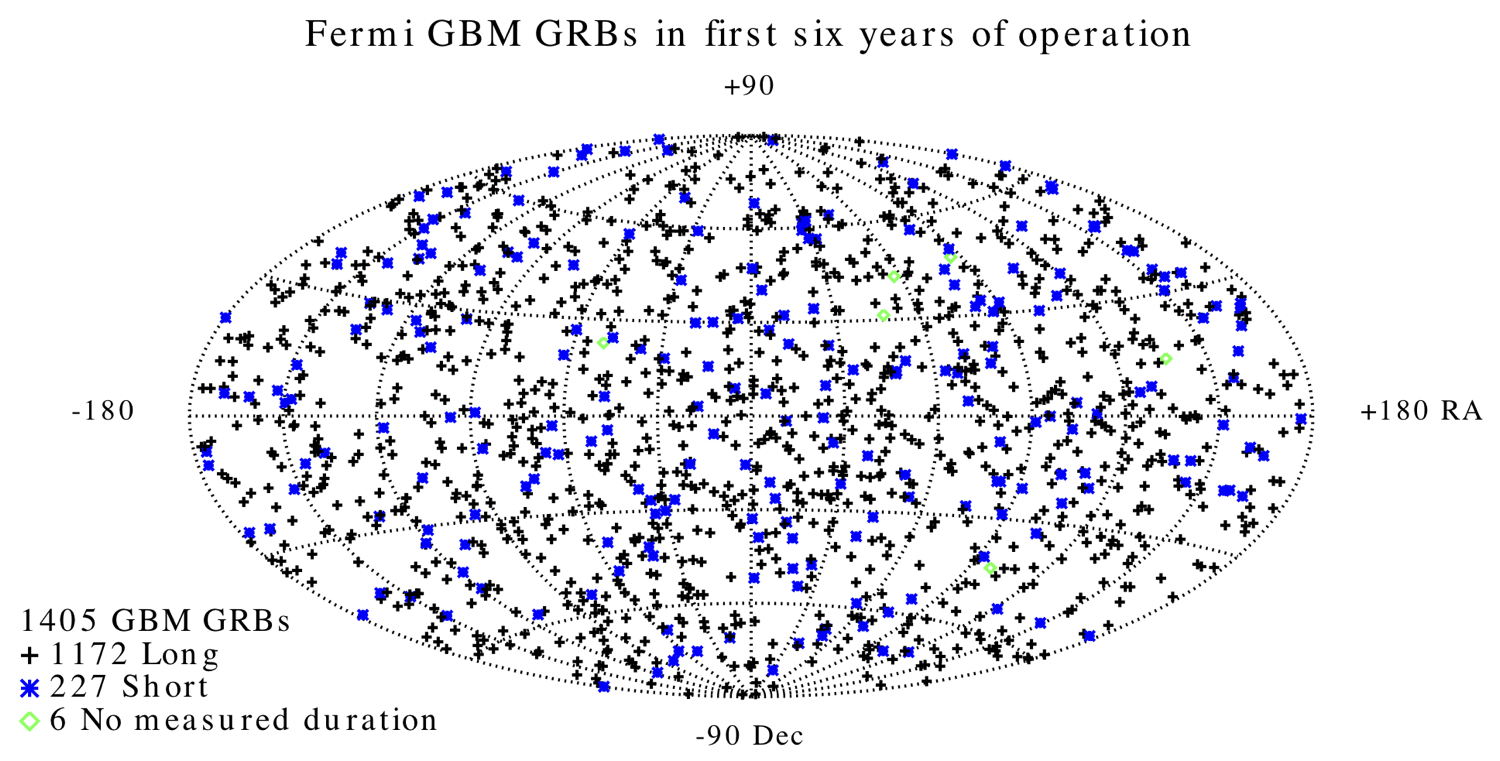
\includegraphics[width=0.9\linewidth]{figures/introduction/grbs.png}
\caption{The distribution of GRBs in the sky as observed by Fermi Gamma-ray Space Telescope in the first six years of operation shows that they are isotropically distributed and independent of their brightness, duration, spectrum, or any other characteristic. Credits to \cite{fermiwebsite}.}
\label{fig:grbs-localization}
\end{figure}
Gamma-ray bursts (GRBs) are among the most intense and energetic transients known to astronomers. They emit a vast amount of energy in a few seconds, equivalent to that emitted by a star like our Sun in its entire lifetime. Their origins have puzzled scientists since they were first serendipitously detected in the late 1960s by the Vela Satellite Network. Initially, it was believed that GRBs were of Galactic origin, but in the early 1990s, it was realized that they are isotropically distributed and have a cosmological origin \cite{mao_paczynski_1992}, \cite{meegan_fishman_wilson_1992}. \autoref{fig:grbs-localization} shows the distribution of GRBs in the sky as observed by Fermi Gamma-ray Space Telescope in the first six years of operation. Since the 1990s, GRBs have been the subject of intensive study, particularly after the Burst and Transient Source Experiment (BATSE) on board the Compton Gamma Ray Observatory began operations. The fluence, or energy per unit area, of a single GRB event ranges from $10^{-7}$ to $10^{-5} erg/cm^2$, and the isotropic energy, or the energy emitted in all directions, ranges from about $10^{48}$ to $10^{55} erg$. This makes GRBs the most violent and energetic stellar explosions known to humankind \cite{Kumar_Zhang_2015}.
The nature of GRBs is still not fully understood, despite many years of research. The fireball model (represented in \autoref{fig:fireball}) is one historical model that explains the mechanism of GRBs. It proposes that they are produced by highly relativistic and collimated jets, and that the interaction of blobs in the jet produces the prompt emission. In contrast, the interaction of the jet with ambient material produces the multiwavelength afterglow \cite{Bhat_2011}. GRBs are traditionally grouped into two categories: short GRBs (SGRBs) and long GRBs (LGRBs), depending on the duration of the burst. In 1997, scientists discovered that long GRBs occur in star-forming regions. This led Paczynski to propose that core-collapse events cause LGRBs \cite{paczynski_1998}. Around the same time, MacFadyen and Woosley proposed the collapsar model, which states that a GRB is produced by a jet that emerges from the center of a collapsing star and penetrates the stellar envelope \cite{macfadyen_woosley_1999}. However, it wasn't until the discovery of \textit{SN2003dh} in association with \textit{GRB030329} that the link between GRBs and supernovae was confirmed \cite{hjorth_et_al_2003}. Since then, several other GRB-SN associations have been discovered, further solidifying the collapsar model as the explanation for LGRBs \cite{bromberg2012observational}. SGRBs are thought to be the result of compact binary mergers with at least one neutron star, such as a black hole and a neutron star (BH-NS), or two neutron stars (NS-NS) \cite{cohen1995distribution}, or two black holes (BH-BH) \cite{Perna_2016}. For this reason, they are also associated with 
gravitational wave (GW) counterparts \cite{abbott_et_al_2017}. The advanced Laser Interferometer Gravitational-Wave Observatory (LIGO) has detected several GWs, including \textit{GW150914}, \textit{GW151226}, \textit{GW170104}, and \textit{GW170817}. The observation of the association of \textit{GW170817} and \textit{GRB170817A} \cite{abbott_et_al_2017} confirms the NS-NS merger as a progenitor of SGRBs.
 \begin{figure}[t]
\centering
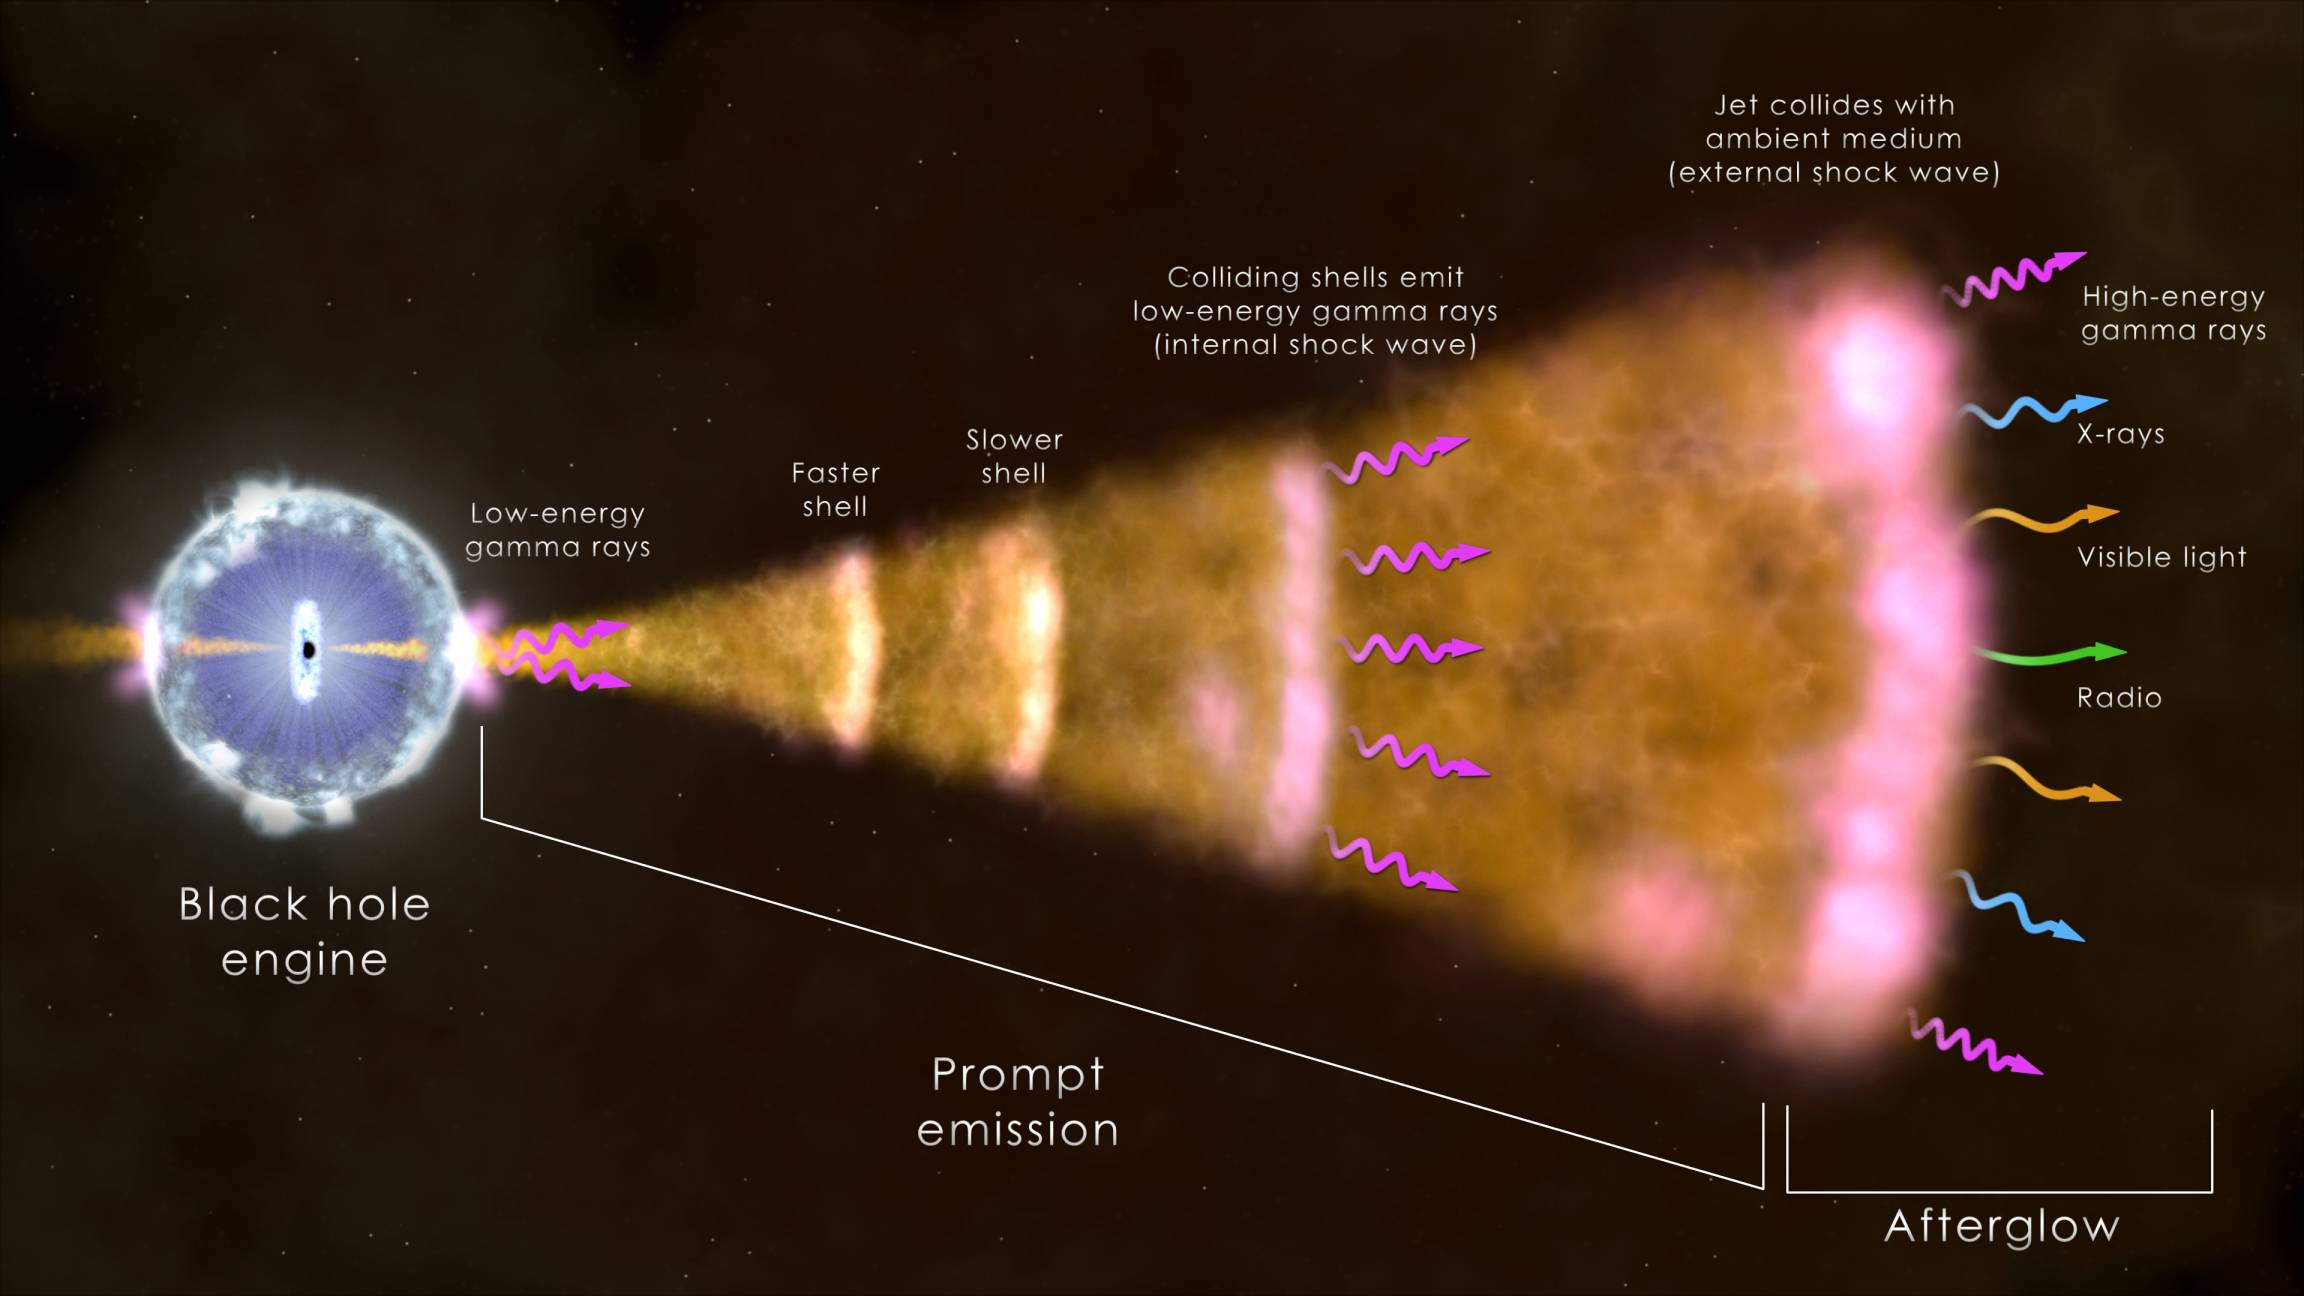
\includegraphics[width=0.9\linewidth]{figures/introduction/grb_fireball.jpg}
\caption{Sketch showing the different phases involved in the \textit{fireball} model with internal shocks producing the $\gamma$-ray prompt emission and external shock with the interstellar medium or the star wind responsible
for the afterglow phase observed in radio, optical, X-rays, and $\gamma$-rays. Credits to \cite{fermiwebsite}.}
\label{fig:fireball}
\end{figure}


\section{Analysis of Gamma-ray data}
\label{s:gamma-ray-data-analysis}
As outlined in \autoref{s:iact}, when a high-energy photon from a $\gamma$-ray source collides with the Earth's atmosphere, it produces an electromagnetic air shower that results in Cherenkov emission, which is then observed with an optical telescope on the ground. The light from the shower triggers the telescope, and the incoming signals are processed and classified to reconstruct the primary event's energy and arrival direction. However, observations are heavily affected by background events caused mainly by cosmic hadrons, so significant effort is required to differentiate between astrophysics events and background noise. The reconstruction outcome is a photon list, a collection of individual photons along with their arrival time, reconstructed direction, and reconstructed energy. The  high-level $\gamma$-ray analysis is carried out at this stage to generate skymaps, spectra, and light curves and finally perform detections. This section will discuss the Full-FoV Maximum Likelihood, Aperture Photometry, and Li\&Ma analysis techniques. Their usage in the real-time scenario has been investigated by \cite{tampieri2020real}, \cite{di2020detection} and \cite{di2021detection}. 

\subsection{The calibration database and the Instrument Response Functions}
\label{ss:caldb}
The calibration database contains \textit{instrument response functions}, required to simulate and analyze CTA event data. The instrument response function (IRF) $R(\bm{p}',E',t'|\bm{p}, E, t)$ describes the transformation from the physical properties of a photon (sky direction $\bm{p}$, energy E, and time t) to the measured characteristics of an event $\bm{p'},E',t'$ (the instrument response function is given in units of $cm^2 sr^{-1} s^{-1} MeV^{-1}$) \cite{Knodlseder_2016}. 
The IRF can be factorized in \textit{effective area} $A_{eff}(\bm{p},E,t)$ in the units of $cm^2$, \textit{point-spread function} $PSF(\bm{p}|p,E,t)$, and \textit{energy dispersion} $E_{disp}(E'|\bm{p},E,t)$. Furthermore, every IRF includes an account of the background rates as they vary in relation to energy and location within the field of view. The background rate is mostly composed of cosmic-ray hadrons and electrons that pass the gamma-ray selection criteria (cuts) \cite{di2020detection}. During a simulation, the response of the instrument is applied to the ideal simulation model  to obtain the data as it was seen by the telescope. Instead, the telescope observation data must be restored during the analysis to obtain the real quantities, considering the IRF.

\subsection{Full Field of View Maximum Likelihood}
\label{ss:ffov-ml}
The likelihood is a mathematical function that quantifies the compatibility of a set of observed data with a given statistical hypothesis or model. It is the probability of obtaining the observed data, assuming the hypothesis is true. The likelihood can be used to estimate a model's parameters by finding the parameters that maximize the likelihood. This method of finding the maximum likelihood estimates of the parameters is called \textit{maximum likelihood estimation}. The method of using likelihood ratio for estimating parameters in high-energy astronomy was first introduced by Cash in the late 1970s \cite{cash_1979}. The first step in applying the Full-FoV Maximum Likelihood analysis is to define a background model, which describes the expected count rate of $\gamma$-rays in the FoV without any sources. This model can be based on the average count rate measured in a nearby region of the FoV or on a more complex model of the $\gamma$-ray background that considers variations in the background due to the telescope's point spread function and other effects. The second step is to define a source model, which describes the expected count rate of gamma rays from a point source. This model can be based on the point spread function (PSF) of the $\gamma$-ray telescope and the spectral properties of the source \cite{di2020detection}. The Full-FoV Maximum Likelihood analysis is a powerful method for detecting $\gamma$-ray sources but has two main limitations:
\begin{itemize}
    \item[1] Assumptions: the method relies on the assumptions that the background and source models are accurate representations of the data, which can limit its ability to detect sources that do not conform to these models.
    \item[2] Computational cost: the method can be computationally expensive, especially when applied to large fields of view or when searching multiple sources.
\end{itemize}
\subsection{Aperture photometry}
\label{ss:aperture-photometry}
Aperture photometry is a method of measuring the flux of gamma rays from a source by determining the number of events recorded in a region of interest called the \textit{on region} and comparing it to an estimate of the residual cosmic-ray background. This estimate is scaled appropriately before the comparison \cite{mohrmann2019}. The on/off method is applied to a list of photons to estimate the source event counts. The method consists in defining an aperture, a closed region centered on the source, to count the on-source photons. The background is estimated by observing one or more off-source regions with no source signals. The number of photons in these regions is the background contribution. It is important to use many large background regions to get good statistics. Still, it is also important to ensure that the background regions share similar characteristics with the source region to avoid contamination. To determine the number of excess photons from the source, the normalized number of off-region events is subtracted from the on-region data. The probable number of photons contributed by the source is calculated using the following formula:
$$NS = N_{on} - \alpha*N_{off}$$
Where $N_{on}$ are the counts in the source region, $N_{off}$ are the counts in the background regions, and $\alpha$ is a background scale factor, to obtain valid background statistics, it is usually necessary to take multiple observations, which introduces additional scaling factors to consider. These factors include the different effective areas (A), exposure (t), and size of the region (k) between the on and off observations. With the counts in the on and off regions, and the excess counts, it is possible to estimate the detection significance, the source flux, and the lightcurve in a simple and fast way without the need for modeling \cite{tampieri2020real}.

\subsection{Li\&Ma}
\label{ss:li-ma}
The Li\&Ma technique is a statistical method used to calculate the significance of a $\gamma$-ray signal. It is used to detect weak signals in the presence of background noise and is considered a standard technique in $\gamma$-ray astronomy. Li\&Ma estimates the significance level with the likelihood ratio method, using the $N_{on}$ and $N_{off}$ photon counts. The null hypothesis has signal $NS = 0$. It is based on the Poisson statistics to develop the likelihood ratio $\lambda$ calculations. Wilks's theorem \cite{wilks_1938} provides an analytical expression for the likelihood ratio that is asymptotically exact. The theorem demonstrates that the $-2$ times the natural logarithm of the likelihood ratio $\lamda$ follows a $\chi^2$ distribution when the null hypothesis is true. Finally, the formula to estimate the significance level is the following: 
$$S = \sqrt{2}{[(N_{on}\ln{(\frac{1+\alpha}{\alpha})(\frac{N_{on}}{N_{on}+N_{off}})} + N_{off}\ln{(1+\alpha)(\frac{N_{off}}{N_{on}+N_{off}})}] }^{\frac{1}{2}}$$
This technique has two main limitations:
\begin{enumerate}
    \item[1] For Wilks' theorem to hold, the statistical bins of the analysis must be independent.
    \item[2] The Li\&Ma article \cite{Lima_1983} proves the significance equation can be applied only with a minimum number of counts: $n_{on} \geq 10$ and $ n_{off} \geq 10$. 
\end{enumerate}


\subsection{Pointing modes}
\label{ss:pointing-modes}
Ground-based very-high-energy $\gamma$-ray telescopes boast impressive sensitivity, but to fully realize their potential, they must address a major source of systematic error: background subtraction. Estimating background is crucial in analyzing $\gamma$-ray data using imaging atmospheric Cherenkov techniques. To perform aperture photometry analysis, it's necessary to count photons in the on-source region and subtract an estimated background. Various techniques can be employed to estimate the background of an observation, each with its advantages and disadvantages. The choice of which method to use depends on the specific requirements of the data analysis and the characteristics of the observation \cite{Berge_2007}. 

\subsubsection{The reflected-region}
\label{ss:reflected-region}
One approach is the reflected-region background model, shown in \autoref{fig:reflected}. The source isn't at the center of the field of view but is displaced with an offset relative to the pointing direction of the telescope. The simplest reflection estimation uses a single off-region in the opposite direction relative to the center of the field, with the exact shape of the on-source region. To improve statistics in background measurements, the method can be expanded by utilizing multiple background regions equidistant from the telescope pointing direction. The sum of the event counts $N_{off}$ from these off regions are used to estimate the background of the on-region, scaled by the number of off regions. The reflected-region background model has the advantage of being independent of the exact shape of the acceptance function. It relies solely on the assumption of radial symmetry of the acceptance. The acceptance function measures a detector's sensitivity to gamma rays as a function of the direction and energy of the incoming gamma ray. It describes how likely a gamma ray will be detected as a function of its direction and energy. The geometric acceptance of the detector, the efficiency of the detector, and the atmospheric absorption of gamma rays typically determine the acceptance function. The radial symmetry of the acceptance assumes that the acceptance function is the same for all directions around a given point in the sky and depends only on the distance from that point. In other words, it assumes that the acceptance function does not change with direction but only with the distance from the center. Hence, this assumption is particularly useful when analyzing data from telescopes where the source is not at the center of the field of view. However, this approach requires a suitable observation strategy. It cannot be applied if the observation positions of a data set are within an extended source region or if there are too many other $\gamma$-ray sources in the field of view. In such cases, one might end up in a situation where it is impossible to define a reflected background region without overlap with a known source region, or, in the case of close-by sources just below the detection limit, one might obtain a $\gamma$-ray contaminated background estimate.
 \begin{figure}[t]
\centering
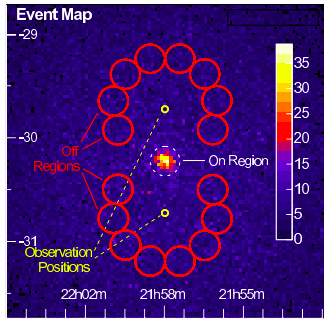
\includegraphics[width=0.7\linewidth]{figures/introduction/reflected.png}
\caption{Count map of $\gamma$-ray-like events with a reflected region background model. Credits to \cite{berger_2014}}
\label{fig:reflected}
\end{figure}
\section{Summary}
\label{s:introduction-summary}


  \newpage
 
  \chapter{Anomaly detection for timeseries data}\label{c:Background-Anomaly-Detection}
  \begin{chapabstract}
\small{
This chapter introduces the concept of anomaly detection for time series analysis, discussing the major existing contributions to the field. This chapter is organized as follows. \autoref{s:anomaly-detection} introduces the definition and properties of time series data and the concept of anomaly. It discusses the several types of techniques existing in the scientific literature, classifying them using a taxonomy. 
\autoref{s:ad-with-dl} focuses on anomaly detection techniques based on deep learning. The method developed in this work belongs to this category.
\autoref{ss:ad-astrophysics} lists several contributions made in the astrophysics field, proving that these techniques are becoming increasingly popular for analyzing astrophysical data.
}\\
\begin{center}
\noindent\makebox[0.8\linewidth]{\rule{0.66\paperwidth}{0.4pt}}
\end{center}
\vspace{1cm}
\end{chapabstract}

\section{Anomaly Detection for time series analysis}
\label{s:anomaly-detection}
Anomaly detection involves the identification of patterns or events in data that are unusual or unexpected compared to a baseline or normal behavior \cite{chandola_2019}. Various factors, such as errors in data collection, rare events, or the influence of external factors, can cause these anomalies. This chapter will discuss anomaly detection in the context of time series data. A time series is generally considered a collection of observations indexed in time order, defined by the following properties:
\begin{itemize}
    \item Temporality (or temporal correlation): if successive data point in the series depends on its past values.
    \item Dimensionality: the number of individual data attributes captured in each observation. In the case of univariate time series, each observation is defined by one data attribute. In contrast, multiple attributes define the observations that compose a multivariate time series. In the latter case, both the temporal dependence and the correlations between data attributes should be considered. Below are the mathematical definitions of a univariate and multivariate time series, assuming that the observations composing a time series have the same temporal granularity.
    \begin{definition} \label{def:univariate-timeseries}
    [Univariate time series] A \textit{univariate time series} $\textbf{X}=\{\textbf{x}_t\}_{t\in T}$ is an ordered set of real-valued observations, where each observation is recorded at a specific time $t \in T \subseteq \mathbb{Z}^+$. 
    \end{definition}
    \begin{definition} \label{def:multivariate-timeseries}
    [Multivariate time series] A \textit{multivariate time series} $\textbf{X}=\{\textbf{x}_t\}_{t\in T}$ is an ordered set of real-valued observations, where each observation is recorded at a specific time $t \in T \subseteq \mathbb{Z}^+$ and consists of k real-valued observations, $\textbf{x}_t = (x_{1t}, .., x_{kt})$. 
    \end{definition}    
    \begin{definition}
    [Subsequence] $\textbf{S}=\{\textbf{x}_p,\textbf{x}_{p+1},..,\textbf{x}_{p+n-1}\}$ is a \textit{subsequence} of length $n \leq |T|$ of a multivariate time series \textbf{X}, for $p,t \in T$ and $p \leq |T| - n + 1$.
    \end{definition}    
    \item Stationarity: a time series is said to be stationary if its statistical properties do not change over time. 
    \begin{definition}
    [Strongly stationary] For any $\tau \in \mathbb{N}$, a continuous stochastic process $\textbf{x}=\{x^t\}_{t \in T \subset \mathbb{Z}^+}$ is strongly stationary if following condition is satisfied:
    $$\bm{F_x}(x^{1+\tau},...,x^{t+\tau})=\bm{F_x}(x^1,...,x^t)$$ 
    where $\bm{F_x}$ denotes the joint distribution function \cite{choi2021deep}.
    \end{definition}    
    Many real-world environments experience changes in their underlying statistical data distribution over time, a phenomenon commonly referred to as concept drift \cite{Widmer_1994}. This can be a significant issue as it can negatively impact the performance of models trained on historical data \cite{Pan_2010}. For example, the \textit{seasonality} is a periodic fluctuation over a limited time scale (e.g., power consumption is high during the day and low during the night, and online sales increase rapidly over the Black Friday weekend and then decrease again). In addition, \textit{change points} are time instants after which the underlying statistical distribution of a stream changes, for example, when operations are stopped and restarted with a different setting. As we will see in the following sections, the scientific literature contains anomaly detection techniques designed to work exclusively with stationary or non-stationary time series, as well as techniques developed for the stationary case and then adapted for the non-stationary setting.
    \item Noise: since it is a common issue in real-world systems, \cite{Tang_2018} adds this property to time series data. The noise is defined as any unwanted signal changes during capture, storage, transmission, processing, or conversion. While noise can often be caused by minor fluctuations in sensor sensitivity and have little impact on the overall data structure, it can make it difficult to distinguish between noise and actual anomalies in a noisy system. This can greatly impact the performance of detection models \cite{Tuzlukov_2002}.
\end{itemize}
     
Before introducing the taxonomy of the anomaly detection techniques for time series data, the definition of anomaly (or outlier) must be given. A widely used definition has been provided by Hawkins \cite{hawkins1980identification}:
\begin{quote}
"An observation which deviates so much from other observations as to arouse suspicions that it was generated by a different mechanism"
\end{quote}
Outliers in time series can have different meanings depending on the context \cite{blazquez2020review}. According to Aggarwal \cite{aggarwal_2016}, they can be seen as noise, erroneous, or unwanted data that are not of interest to the analyst. In these cases, it is best to delete or correct them to improve the data quality. However, in recent years, researchers have increasingly focused on detecting and analyzing unusual but interesting (for a specific domain) phenomena, such as the case of fraud detection. These outliers are often referred to as anomalies. This chapter will refer to this meaning and from now on, the term anomaly will be used. 

The scientific literature proposes numerous anomaly detection techniques applied to time series analysis \cite{chandola_2019}, \cite{blazquez2020review}, \cite{choi2021deep}, \cite{Garg_2021}. In \cite{blazquez2020review} review paper, the anomaly detection techniques are grouped along three axes. The first axis refers to the capability of analyzing univariate or multivariate time series. The second axis refers to the type of anomaly to be detected. Anomalies in time series data can take several forms. A point anomaly is an unusual data point in a specific time instant compared to other values in the series (global) or neighboring points (local). These anomalies can occur in one variable (\textit{O1, O2} in \autoref{fig:point-anomaly}, left panel) or multiple variables (\textit{O1, O2, O3} in \autoref{fig:point-anomaly}, right panel). Another type of anomaly is called subsequence, which refers to consecutive points in time that exhibit unusual behavior together, even if each point is not necessarily an anomaly. These can also be global or local and affect one variable (\textit{O1, O2} in \autoref{fig:subsequence-anomaly}, left panel and \textit{O3} in \autoref{fig:subsequence-anomaly}, right panel) or multiple variables (\textit{O1} in \autoref{fig:subsequence-anomaly}, right panel). Finally, the entire time series can be considered anomalous when multiple variables are involved (\textit{Variable 4} in \autoref{fig:timseries-anomaly}). Although these definitions of anomalies are general and usable in different real-life scenarios, the classification of what is considered abnormal varies based on one's perspective of what is considered normal. Hence they may be further subdivided into more specific groups \cite{choi2021deep}, \cite{Tang_2018}. 

\begin{figure}[t]
\centering
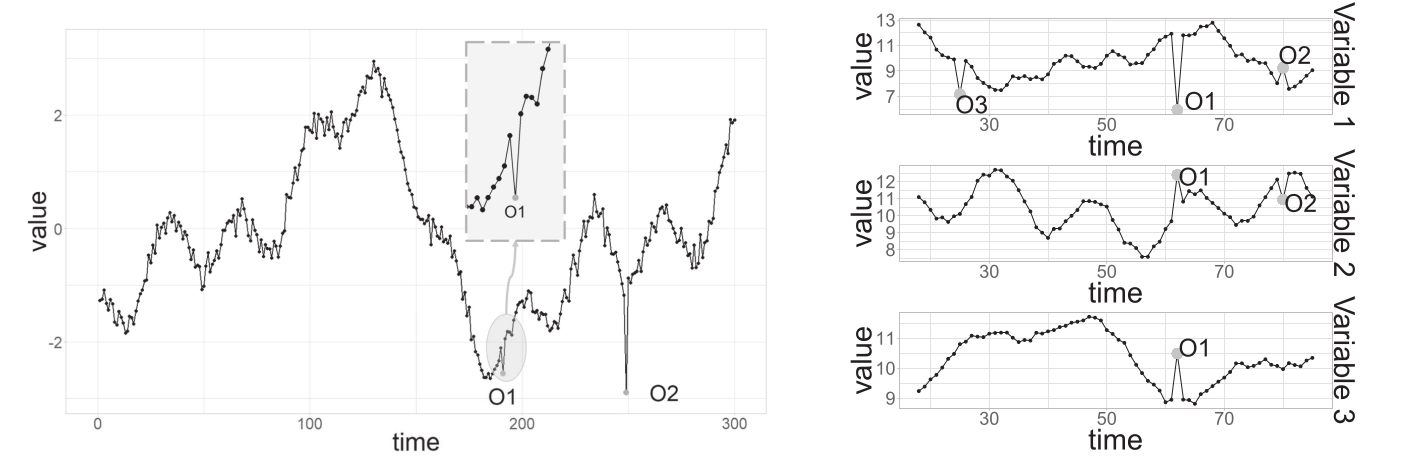
\includegraphics[width=1\linewidth]{figures/introduction-2/point-anomaly.png}
\caption{Point anomalies in time series data. Left panel: univariate time series. Right panel: multivariate time series. Credits to \cite{blazquez2020review}.}
\label{fig:point-anomaly}
\end{figure}
\begin{figure}[t]
\centering
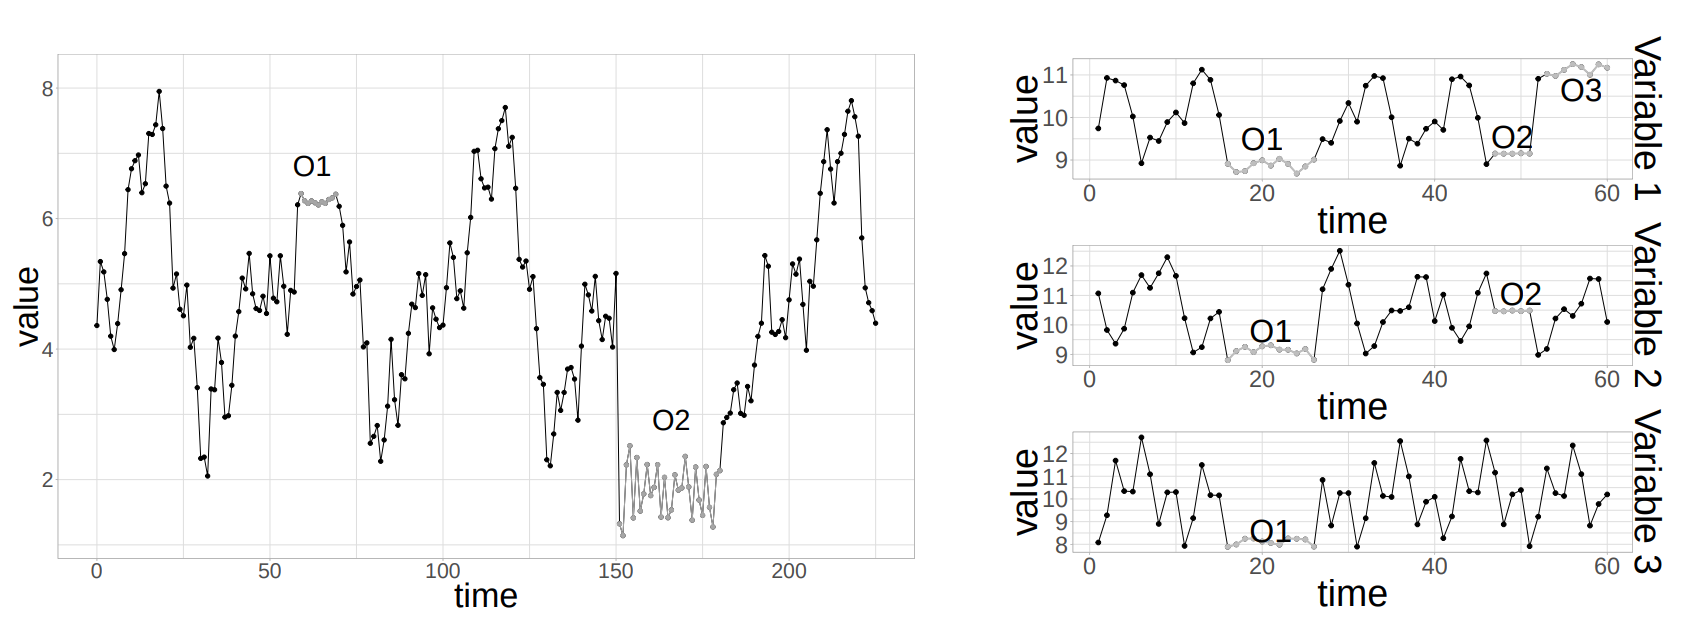
\includegraphics[width=1\linewidth]{figures/introduction-2/subsequence-anomaly.png}
\caption{Subsequence anomalies in time series data. Left panel: univariate time series. Right panel: multivariate time series. Credits to \cite{blazquez2020review}.}
\label{fig:subsequence-anomaly}
\end{figure}
\begin{figure}[t]
\centering
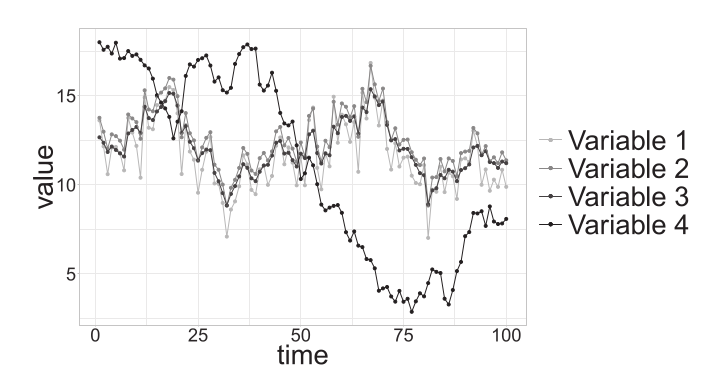
\includegraphics[width=0.6\linewidth]{figures/introduction-2/timseries-anomaly.png}
\caption{Anomalous time series (\textit{Variable 4}) in a multivariate time series. Credits to \cite{blazquez2020review}.}
\label{fig:timseries-anomaly}
\end{figure}

The third dimension of the taxonomy examines the type of detection method used. A univariate detection method only examines one variable over time, while a multivariate method can analyze multiple variables simultaneously. It's worth noting that even though the input data may be a multivariate time series, a univariate detection method can still be employed by analyzing each variable individually, disregarding any potential dependencies between them. However, a multivariate technique cannot be utilized with univariate time series data. Therefore, this dimension only applies to multivariate time series data.

The three dimensions described above are the top nodes of the proposed taxonomy. The authors of \cite{blazquez2020review} further develop the proposed taxonomy tree. In contrast, in \cite{choi2021deep}, the anomaly detection techniques are divided into two main groups: \textit{traditional approaches} and \textit{deep learning based}. The following sections will continue to describe the taxonomy proposed in \cite{blazquez2020review} and then focus on deep learning-based methods mentioned in \cite{choi2021deep}.

\subsection{Anomaly detection techniques for point anomalies in the univariate domain}
\label{ss:point-anomalies-univariate}
The set of anomaly detection techniques that can detect point anomalies is further divided by \cite{blazquez2020review}, taking into account the following aspects:
\begin{itemize}
    \item The technique exploits the \textbf{temporality} of the data: some techniques take into account the temporal ordering of observations, and others completely disregard this information. The latter will produce the same results even when the observations are shuffled.
    \item The technique can be applied in a \textbf{streaming} context: some techniques can identify outliers in real-time, as soon as new data points arrive, without needing to wait for further data. Among these methods, some maintain a constant model throughout the stream. In contrast, others adapt and update their detection models with new information, either by completely retraining the model or through incremental learning. Techniques that cannot make instant decisions on new data points are considered unsuitable for streaming time series analysis.
    \item The \textbf{nature} of the technique: \textit{model-based} techniques rely on fitting a model; \textit{density-based} techniques use the concept of neighborhood; \textit{histogramming} techniques compute a histogram representation of the data. 
\end{itemize}
The next sections will describe further the last point of the previous listing.

\subsubsection{Model-based techniques}
\label{ss:model-based}
The model-based techniques are the most commonly used approach in literature and rely on fitting a model to estimate the expected value of a data point \cite{blazquez2020review}. The data point is considered an anomaly if: 
\begin{definition}\label{def:model-based}
    $|x_t - \hat{x}_t| > \tau $, where $x_t$ is the observed data point and $\hat{x}_t$ is its expected value and $\tau$ is a threshold.
\end{definition}
The expected value, $\hat{x}_t$, represents the typical or normal value of a data point in the time series, and the threshold $\tau$ represents the level of deviation from this normal value considered abnormal or significant. As we will see later in this chapter, \cite{choi2021deep} generalizes this concept with the definition of the \textit{anomaly score}, a numerical value that indicates the likelihood of a data sample being anomalous that replaces the term $|x_t - \hat{x}_t|$ in \autoref{def:model-based}. Despite calculating the expected value $\hat{x}_t$ or the anomaly score and threshold $\tau$ differently, these techniques involve explicitly or implicitly fitting a model. Model-based techniques are divided into \textbf{estimation} (shown in \autoref{fig:model-based}, left panel) and \textbf{prediction} techniques (shown in \autoref{fig:model-based}, right panel). Estimation techniques use $\{x_{t-k_1},...,x_t,...,x_{t+k_2}\}$ to compute $\hat{x}_t$, while in prediction techniques, $\hat{x}_t$ is computed using only previous observations. The main practical difference between the two is that prediction techniques can be applied in the streaming scenario as they can immediately identify whether a new data point is an outlier as soon as it arrives. In contrast, estimation techniques can only do so if only the current point $x_t$ is used to compute the expected value along with some preceding points. 
\begin{figure}[t]
\centering
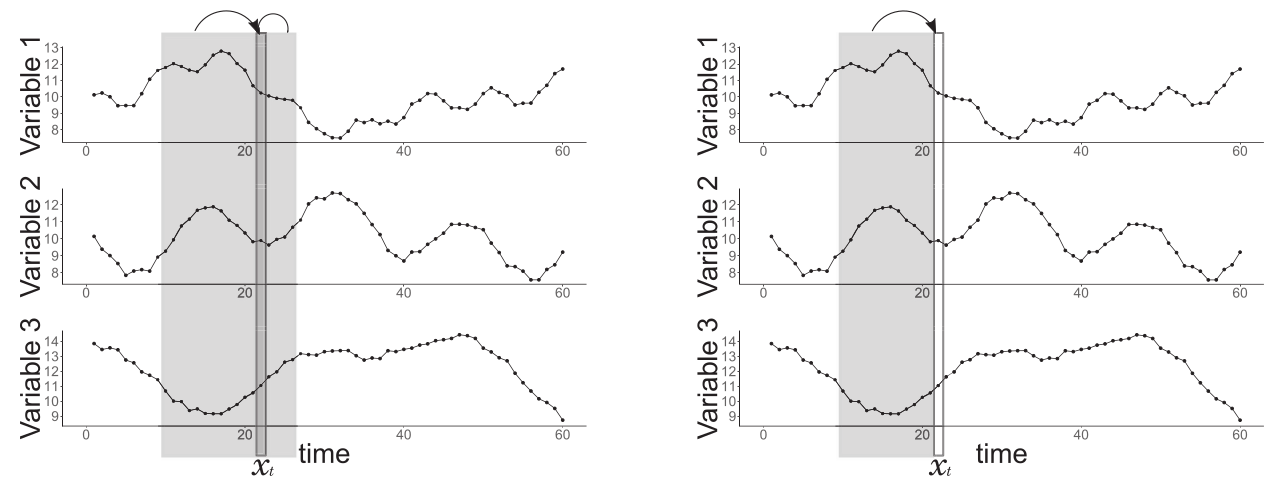
\includegraphics[width=1\linewidth]{figures/introduction-2/model-based.png}
\caption{Example of estimation (left panel) and prediction (right panel) models-based approach for a multivariate time series. Consider only one variable for the univariate scenario. Credits to \cite{blazquez2020review}.}
\label{fig:model-based}
\end{figure}


\subsubsection{Density-based techniques}
The basic idea behind this method is that normal data points will be closely packed together, forming dense clusters. Anomalous data points, on the other hand, will be located in areas of the data where there are few other data points, resulting in a lower density of data in that region. The \textit{density-based} approach relies on computing the density of data points in different regions of the data and identifying any regions with a lower density than the surrounding areas, flagging them as potential anomalies. This approach can be applied to data of any dimensionality and does not rely on prior knowledge of the normal behavior of the data \cite{blazquez2020review}.


\subsubsection{Histogramming techniques}
The method in question is centered around identifying points in a time series that, when removed, result in a histogram representation with less error than the original, even when the number of buckets is decreased to allow for the storage of these points separately (\autoref{fig:histogramming}). This approach aims to detect the points in the time series that deviate from the expected behavior, and removing them allows for a more accurate representation of the data \cite{blazquez2020review}.
\begin{figure}[t]
\centering
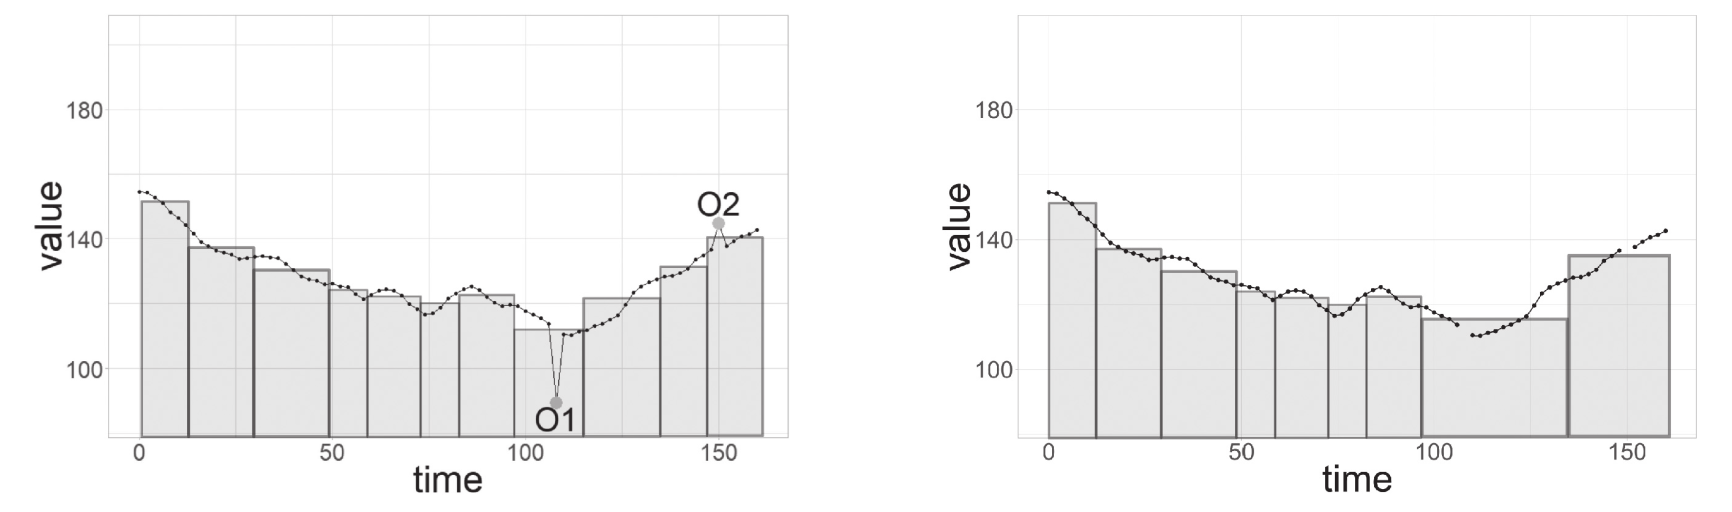
\includegraphics[width=1\linewidth]{figures/introduction-2/histogramming.png}
\caption{Example of the histogramming technique for univariate time series. The points $\{O1, O2\}$ are anomalous. Credits to \cite{blazquez2020review}.}
\label{fig:histogramming}
\end{figure}

\subsubsection{Parametric vs non-parametric techniques}
In \cite{blazquez2020review}, the authors further develop the taxonomy tree taking into account the parametric and non-parametric nature of the techniques. Parametric techniques assume that the underlying distribution of the data belongs to a specific family of distributions and estimate a fixed number of parameters from the data. On the other hand, non-parametric methods do not make any assumptions about the underlying distribution and instead determine the model or family of distributions from the data with a flexible number of parameters. Additionally, there are semi-parametric methods that combine elements of both parametric and non-parametric approaches. In general, the term \textit{anomaly} describes the data points that deviate from the expected behavior. The techniques discussed consider the temporal aspect of the data and can be applied in a streaming context. Additionally, some iterative methods are used to identify and improve the quality of the time series data. Most of the model-based techniques are either parametric or semi-parametric. Semi-parametric techniques typically assume a distribution over the residuals when determining a threshold value, even if the residuals are obtained through a non-parametric approach.

\subsection{Anomaly detection techniques for point anomalies in the multivariate domain}
Multiple variables may be correlated when the input data is composed of multivariate time series. Unlike the case of univariate time series, the detection method used for identifying point outliers in multivariate time series should handle not only a single variable but also multiple variables at once. 
Furthermore, an outlier in a multivariate time series can simultaneously impact one or multiple variables. The set of anomaly detection techniques that can detect point anomalies in the multivariate domain is further divided into two groups by \cite{blazquez2020review}, taking into account the type of analysis: a univariate analysis for each variable to detect univariate point outliers, without considering dependencies that may exist between the variables, or a multivariate analysis, to exploit the correlation dependencies between the variables. Regarding the first case, the techniques described in \autoref{ss:point-anomalies-univariate} can be applied. To overcome the loss of information that occurs when the correlation dependencies between the variables are not considered, dimensionality reduction steps, such as PCA, can be used to find a new set of uncorrelated variables where univariate techniques can be applied. Model-based techniques (prediction and estimation models) and histogramming techniques can be extended to carry out the multivariate analysis. Another model-based technique not cited by \cite{blazquez2020review} but used in the literature (see \autoref{ss:ad-astrophysics}) is called \textit{iForest}, from \cite{Liu_2008}, which is fundamentally different from existing approaches as it explicitly isolates anomalies instead of constructing a profile of normal instances. iForest uses sub-sampling and has a linear time complexity with low constant and memory requirements. It works well, especially in large data sets and high-dimensional problems with many irrelevant attributes. In addition, dissimilarity-based techniques are introduced by \cite{blazquez2020review}.

\subsubsection{Dissimilarity techniques}
\label{ss:dissimilarity-univariate}
These methods involve calculating the difference between multiple points or their representations without needing a model to be fitted. For a set threshold value, if the dissimilarity between a point and its expected value exceeds that threshold, the point is considered an outlier. 
\begin{definition}\label{def:model-based}
    $s(x_t, \hat{x}_t) > \tau $, where $x_t$ is the k-dimensional data point and $\hat{x}_t$ is its expected value and $s$ measures the dissimilarity between two multivariate points.
\end{definition}
These techniques typically do not use raw data but instead employ different representation methods, such as graphs or vectors, and the definition of the dissimilarity function $s$ changes accordingly.



\subsection{Anomaly detection techniques for subsequence anomalies in the univariate domain}
\label{ss:ad-subsequence-univariate}
Subsequence anomalies are the second type of anomaly defined by \cite{chandola_2019}. The objective is to spot a sequence of consecutive points that deviate from normal behavior. In this case, we need to take into account additional aspects. 
\begin{itemize}
    \item First and foremost, unlike point anomalies, subsequences consist of multiple points, introducing a new analysis constraint, i.e., the capability to simultaneously analyze subsequences of varying lengths or rely on fixed-length subsequences. In the latter case, a sliding window over the time series can be used to obtain them. It's also worth noting that the number of subsequences the method will consider and analyze is dependent on the chosen length (i.e. the shorter the length, the higher the number of subsequences). 
    \item Another aspect that subsequence anomaly detection methods must consider is the representation of the data. Since comparing subsequences is more challenging and costly than comparing individual points, many techniques use a representation of the subsequences instead of the raw values, such as the \textit{discretization} method, as shown in \cite{Chandola_2012}.
    \item In addition, the subsequence anomalies can be periodic, making their detection more challenging. Periodic subsequence anomalies are unusual sequences that repeat over time.
    \item Furthermore, instead of point anomaly detection, where some methods do not consider temporal dependencies, subsequences inherently consider temporality.
    \item Finally, when analyzing subsequence anomalies in a streaming context, several approaches can be considered: a single data point arrives, and a classification must be given for a subsequence containing this new point; a subsequence arrives, and it needs to be classified; a batch of data arrives, and subsequence anomalies need to be found within it.
\end{itemize}
In this scenario, the anomaly detection techniques belong to the following groups: 
\textit{discord detection} techniques compare each subsequence to all others using the Euclidean distance and require the user to specify the length of the subsequence. These methods are limited because they cannot specify whether the identified subsequences are anomalies. 
The \textit{dissimilarity-based} techniques in the multivariate scenario use a reference of normality to decide whether or not a subsequence is an anomaly based on their direct comparison. This can be defined as:
\begin{definition}\label{def:dissimilarity-based-multivariate}
    $s(S, \hat{S}) > \tau $, where S is the subsequence being analyzed or its representation, $\hat{S}$ is the expected value of $S$ obtained based on the reference of normality, and $s$ measures the dissimilarity between two subsequences.
\end{definition}
\autoref{fig:dissimilarity} shows some examples of different references of normality ($\hat{S}$ in \autoref{def:dissimilarity-based-multivariate}). The subsequence under analysis ($S$ in \autoref{def:dissimilarity-based-multivariate}) and the references are then clustered, and the centroids or center of the cluster to which the $S$ belongs are computed to identify anomalies (as shown in \autoref{fig:clustering}). The dissimilarity-based techniques in the multivariate scenario differ from those introduced in \autoref{ss:dissimilarity-univariate} because of the representations used to describe subsequences (graphs and vectors against clustered representations).
\begin{figure}[t]
\centering
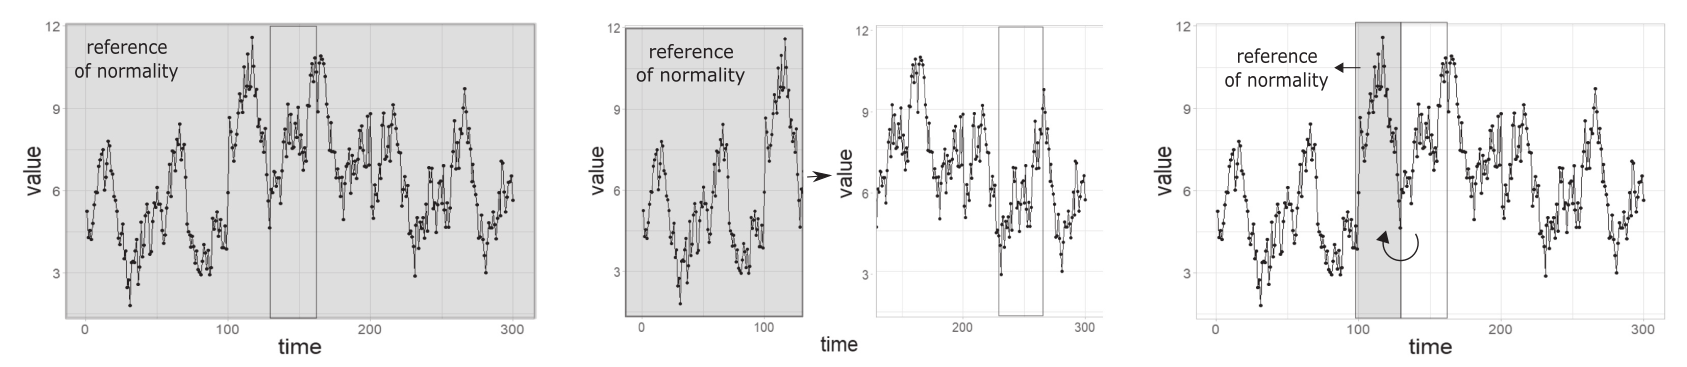
\includegraphics[width=1\linewidth]{figures/introduction-2/dissimilarity.png}
\caption{Example of different references of normality used by dissimilarity-based approaches. The panel on the left shows the same time series. The panel in the middle shows an external time series. The panel on the right shows a previous subsequence. Credits to \cite{blazquez2020review}.}
\label{fig:dissimilarity}
\end{figure}
\begin{figure}[t]
\centering
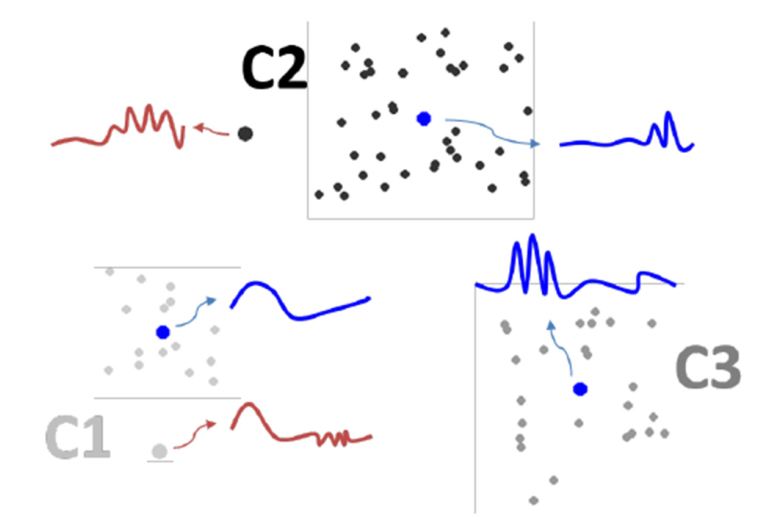
\includegraphics[width=0.5\linewidth]{figures/introduction-2/clustering.png}
\caption{Clustering of the subsequences in a univariate time series. Cluster centroids are highlighted, and C1
and C2 clusters contain subsequence outliers. Credits to \cite{blazquez2020review}.}
\label{fig:clustering}
\end{figure}
The \textit{prediction model-based} techniques in the multivariate scenario build a regression model using past data to predict up to n points into the future. Then, anomalies are detected by calculating the distance from the predicted subsequences to the actual ones. If the distance exceeds a threshold $\tau$ the subsequence is classified as an anomaly. The 
 \textit{frequency-based} techniques compare subsequences to a reference to normality, as done by  \autoref{fig:dissimilarity}. A subsequence $S$ is an
outlier if its frequency is lower than the expected one:
\begin{definition}\label{def:frequency-based}
    $|f(S) - \hat{f}(S)| > \tau $, where $f(S)$ is the frequency of occurrence of $S$, $\hat{f}(S)$ its expected frequency, and $\tau$ a predefined threshold.
\end{definition}
Finally, the last group of multivariate subsequence anomaly detection techniques is based on \textit{information theory}, similar to the frequency-based methods. The main idea is to find patterns in data that happen less often but still happen regularly concerning a reference to normality. Patterns that happen less often are more surprising and carry more information. This can be achieved by looking at how often the symbols in a pattern appeared in the series and how often the pattern appeared overall. 

\subsection{Anomaly detection techniques for subsequence anomalies in the multivariate domain}
\label{ss:ad-subsequence-multivariate}
The techniques mentioned by \cite{blazquez2020review} in this scenario share similar concepts with the technique to detect subsequence anomalies in the univariate domain, as they are simply an advanced version of simpler techniques that have already been discussed earlier. In particular, \textit{model-based} techniques, both prediction and estimation models, performs the best in this scenario, especially if based on deep learning. The following section will focus on this group of techniques.


\section{Anomaly detection with deep learning}
\label{s:ad-with-dl}
To understand why deep learning in unsupervised settings has a critical role in the anomaly detection context, we have two consider two main challenges, described in \cite{choi2021deep}. The first is the rarity of the anomalies. This scarcity makes it time-consuming and resource-intensive to gather enough data for supervised datasets. Additionally, when labeled data is obtained, the imbalance between normal and abnormal data can negatively impact the training of models. In addition, for most real-life use cases, it is not guaranteed to be able to generate a supervised dataset fully representative of the anomalous class. Another challenge regards the complexity of the data. Univariate time-series analysis is still relevant in applications that require minimal computation, such as edge computing. However, as automation and control systems become more complex, it becomes impractical to monitor individual univariate data streams separately. With many dimensions, traditional approaches often experience a decline in performance due to the \textit{curse of dimensionality}. Furthermore, correlations between variables that cannot be inferred through univariate time-series analysis can also indicate anomalies. 



\subsection{Deep learning architectures for anomaly detection in multivariate time series}
The past behavior of a sequence holds valuable information that can indicate potential changes in the future, and deep learning architecture can natively model the temporal context of the data. A popular method is using Recurrent Neural Networks (RNN) and other variants, such as Long Short-Term Memory (LSTM) \cite{Hochreiter_1997} and Gated Recurrent Unit (GRU \cite{Chung_2014}. Those architectures address the vanishing or exploding gradient problem, which occurs when the gradient becomes too small or too large as the network becomes deeper. Through several \textit{gates}, they can learn long-term dependencies by deciding which previous states to keep or discard at each time step. Another approach is the dilated RNN \cite{Chang_2017}, which extracts multi-scale features and models long-term dependencies by using a skip connection between hidden states. While Recurrent Neural Networks (RNNs) are commonly used for analyzing time series data, some studies have found that Convolutional Neural Networks (CNNs) can perform better in certain scenarios that involve short-term data \cite{choi2021deep}. CNNs utilize multiple layers of convolutions, which allow them to learn increasingly complex features as they progress through the layers. 
Additionally, pooling layers introduce non-linearity to the CNNs, allowing them to capture complex patterns \cite{Albawi_2017}. However, a drawback of using CNNs is that it can be challenging to understand patterns that occur over a prolonged period. To address this issue, Temporal Convolutional Networks (TCN) have been proposed by \cite{Lea_2016}. TCN has three distinct characteristics; it uses causal convolutions, meaning that future information is not considered when analyzing past data. It can handle input sequences of any length, similar to RNNs. Furthermore, it can look far into the past using deep networks and dilated convolutions to make predictions. A hybrid architecture, called ConvLSTM, has been introduced by \cite{Shi_2015} to address the spatiotemporal sequence-forecasting problem, i.e., when there's the need to consider the spatial information and temporal dependencies simultaneously.
The spatial information is introduced when a multivariate time series is represented as a 2D covariance matrix. Those matrices are stacked when the time series is monitored with a sliding window, as explained in \cite{choi2021deep}. Recent architectures based on the attention layers \cite{Vaswani_2017}, such as Transformers and bidirectional encoder representations from transformer (BERT) \cite{Devlin_2018}, have been widely used in the field of natural language processing and have recently been applied to the time-series anomaly detection domain due to their ability to handle long-range dependencies effectively. Hierarchical Temporal Memory (HTM) \cite{Hawkins_2016} is a relatively new approach to deep learning architecture and is still being actively researched. HTM has a biologically-inspired design, as it is based on the structure and function of the neocortex, which is the part of the brain responsible for sensory perception, cognition, and decision-making. HTM comprises a hierarchy of layers containing a set of cells organized into columns. The cells in each column are connected to one another and to cells in adjacent columns. The input and the previous states of the connected cells activate the columns. This allows the algorithm to learn and recognize spatial and temporal patterns, making it useful for various applications, including anomaly detection. In addition, one of the key advantages of HTM is its ability to learn and adapt to changing data patterns, making it useful for real-time applications. 

\subsubsection{Anomaly criteria}
\label{ss:anomaly-criteria}
\begin{figure}[t]
\centering
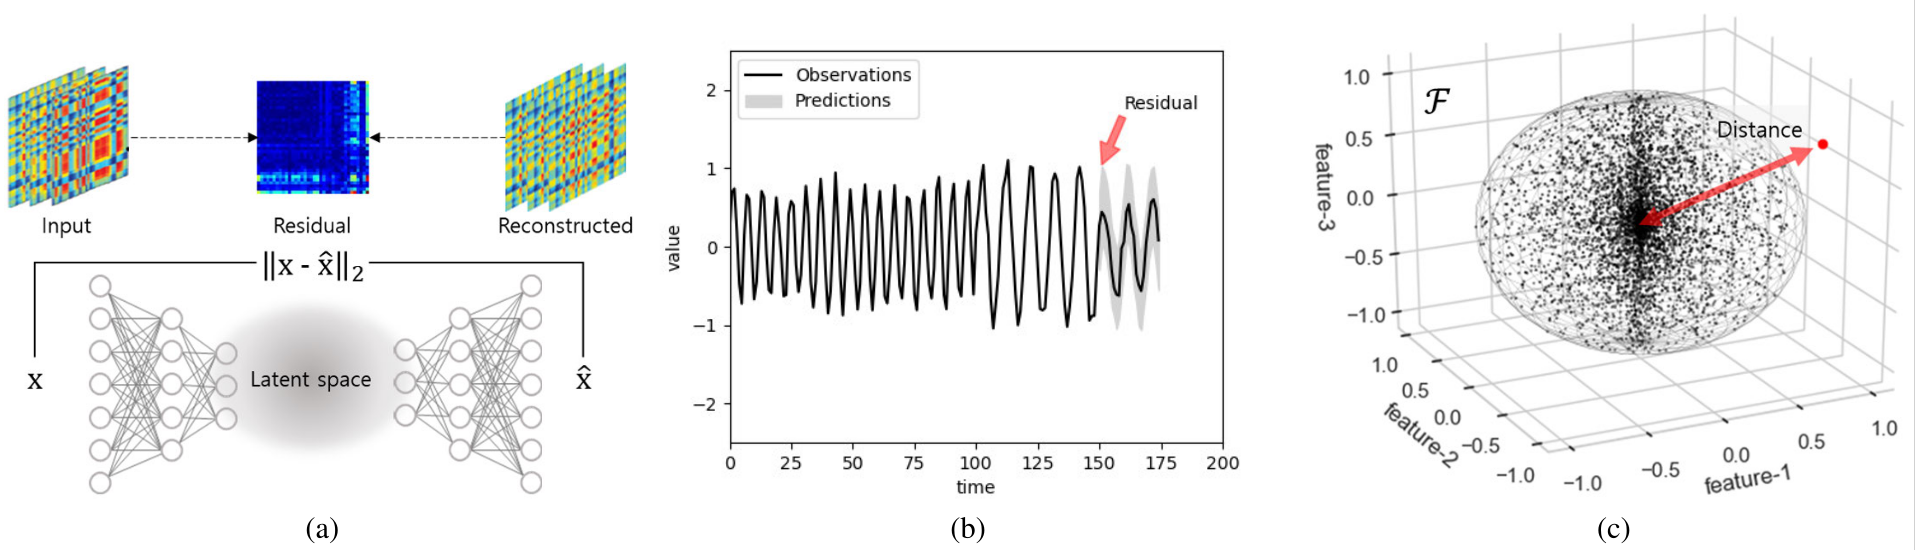
\includegraphics[width=1\linewidth]{figures/introduction-2/anomaly_criteria.png}
\caption{Examples of the anomaly criteria: (a) a reconstruction error; (b) a prediction error; and (c) a dissimilarity. Credits to \cite{choi2021deep}.}
\label{fig:anomaly-criteria}
\end{figure}
The anomaly detection techniques based on deep learning are subdivided into three main categories by \cite{choi2021deep}, concerning the criteria they use to define anomalies. Those techniques all belong to the \autoref{ss:model-based} category introduced in \cite{blazquez2020review}. As outlined in \autoref{ss:model-based}, a model-based technique relies on fitting a model. In this case, a loss function must be defined and minimized since \textit{backpropagation} is used as the learning algorithm. This objective function differs concerning the architecture used. Once the model is trained and the data representation is learned, it is applied to production data to perform inference. The model's output is used to compute an \textit{anomaly score}, i.e., a numerical value that indicates the likelihood of a data sample being anomalous. If the indicator it's greater than a threshold $\tau$, the sample is classified as anomalous. The strategies to compute the anomaly score can be divided into three types: the first is called \textit{recostruction error} and it's a generalization of the estimation-based method described in \autoref{ss:model-based}. This anomaly score is commonly used by AE, VAE, GAN and Transformers. They reconstruct or generate data analogous to the input data and compute the residual between the input and generated data, as shown in \autoref{fig:anomaly-criteria}, panel (a). Prediction techniques compute $\hat{x_t}$ using only previous observations. Obtaining anomaly scores involves assigning a binary label according to the chance of the data point being deemed normal, as outlined in [116], [119]. The discrepancy between the predicted label and actual label demonstrates the prediction error. This method can not always be applied since labels are insufficient in many real-world scenarios. Another method to obtain anomaly scores from prediction models is very similar to \autoref{def:model-based}: the model forecasts the predicted value for future time steps and the anomaly score is computed as the difference between the expected value and the actual data. The latter strategy is shown in \autoref{fig:anomaly-criteria}, panel (b). Finally, the third category contains \textit{dissimilarity-based} methods that extract features from the input data, create clusters, and assess the distance between from the cluster of previous data. This dissimilarity-based method evaluates the similarity through different measures, including the Euclidean distance, Minkowski distance, cosine similarity, and Mahalanobis distance. \cite{choi2021deep} contains several references to techniques that implement the anomaly criteria described above. 

\section{Anomaly detection in astrophysics}
\label{ss:ad-astrophysics}
As automation and technological advancements spread across industries, many systems produce vast amounts of high-dimensional data. As shown by \cite{chandola_2019}, \cite{blazquez2020review}, \cite{choi2021deep}, and \cite{Garg_2021} review papers, anomaly detection techniques are being used in a wide range of contexts, such as identifying fraud in financial transactions, detecting defects in manufacturing processes, identifying cyber attacks in network security, and detecting diseases in medical imaging. These techniques are particularly useful in high-dimensional datasets where manual inspection is infeasible. and when labeled data is unavailable. However, most implementations are highly specific to the individual use case and thus require domain knowledge for appropriate deployment \cite{choi2021deep}. 

The astrophysics domain has the same characteristics: a massive amount of high-dimensional data is being produced, and generating fully-representative supervised datasets is not always feasible due to limited computational resources but also the difficulties in considering all possible sources of systematics, including glitches \cite{Sadeh_2020}, and all possible anomalies, that may be unknown.

Several anomaly detection techniques are used in different astrophysics domains, from traditional methods such as PCA or Isolation Forest to deep learning-based methods. In \cite{Pruzhinskaya_2019}, the photometric data of the Open Supernova Catalog (OSC) is analyzed with dimensionality reduction, and anomalies are detected with the isolation forest algorithm. The latter technique is also the backbone of \textit{Astronomaly} \cite{Webb_2020}, \cite{Lochner_2021}, a general anomaly detection framework with a novel active learning approach designed to provide personalized recommendations for astronomical data, including images, light curves, and spectra. An anomaly detection algorithm based on an unsupervised Random Forest is proposed by \cite{Baron_2017}, which is tested on more than two million galaxy spectra from the Sloan Digital Sky Survey. Furthermore, techniques based on clustering are proposed in the literature \cite{Sadr_2019}, \cite{Giles_2019}. In \cite{Doorenbos_2021}, the performance of six unsupervised outlier detection methods, including the Local Outlier Factor, Isolation Forest, k-means clustering and a convolutional autoencoder, are being compared for the analysis of images from the Sloan Digital Sky Survey. Deep learning-based techniques are also being used: \cite{Ichinohe_2019} proposes an anomaly detection technique based on a variational auto-encoder for high-resolution X-ray spectroscopy, \cite{Margalef_2020} explores the use of deep generative networks for detecting outliers in astronomical imaging data sets, \cite{Zhang_2018} and \cite{Sadeh_2020} use Long Short-term Memory (LSTM). In particular, \cite{Sadeh_2020} proposes a new data-driven discovery framework developed to detect and characterize explosive astrophysical transients using multiple messengers such as neutrinos, optical supernovae, and gamma-rays. Finally, \cite{Marianer_2021} uses semi-supervised outlier detection algorithms to search for unmodelled gravitational wave (GW) signals.
  \newpage
   
  \chapter{Anomaly detection method to perform source detection}\label{c:Contribution}
  \begin{chapabstract}
\small{
This chapter presents the proposed method to address the real-time source detection problem introduced in \autoref{s:sag}. This chapter is organized as follows. \autoref{s:contribution} will describe the proposed anomaly detection technique. It presents the data pipeline that has been developed to generate input data, the deep learning architectures that have been investigated, and the training process. The evaluation of the models will be addressed in \autoref{s:Experiment-Setup}. \autoref{ss:p-values} will describe the p-value analysis to associate each positive classification with a gaussian statistical significance. \autoref{s:non-stationary-settings} will investigate several problems that can arise during the telescope observations and how those problems can affect the proposed system. 
}\\
\begin{center}
\noindent\makebox[0.8\linewidth]{\rule{0.66\paperwidth}{0.4pt}}
\end{center}
\vspace{1cm}
\end{chapabstract}
\section{The proposed anomaly detection method}
\label{s:contribution}
This section will describe the proposed anomaly detection technique. As explained in \autoref{s:anomaly-detection}, the goal of anomaly detection is the identification of rare items, events, or observations which deviate significantly from the majority of the data and do not conform to a well-defined notion of normal behavior.
This work applies anomaly detection analysis to light curves in the gamma-ray energy spectrum. The y-axis represents the \textit{flux} quantity,  describing how much light a source emits per unit of time and surface. The goal is to identify high-energy phenomena called \textit{Gamma-Ray Bursts} (GRBs), described in \autoref{s:Gamma-Ray-Bursts}. This problem is called \textit{source detection}, and it will be framed into the two  use cases of \textit{serendipitous discoveries} (\autoref{s:serendipitous-discoveries}) and \textit{follow-up observations} (\autoref{s:follow-up-observation}) that require real-time analysis of the data. The problem can be addressed by using an anomaly detection approach considering the \textit{normal data} as the signal coming from a sky region where no sources are present except the background. In contrast, \textit{anomalous data} is defined as the signal coming from a sky region where an astrophysical source is present (along with background).
The proposed method belongs to the model-based family of techniques to detect multivariate sub-sequence anomalies described in \autoref{ss:ad-subsequence-multivariate}. It is based on an autoencoder that learns the time series behavior of normal samples. It thereafter uses reconstruction error as anomaly criteria (\autoref{ss:anomaly-criteria}) to detect anomalies. 
Consider a time series $\bm{X} = \{\bm{x_1}, \bm{x_2}, ..., \bm{x_L}\}$ of length $L$, where each point $\bm{x_i} \in \mathbb{R}^3$ is a 3-dimensional vector of flux values. As we will see in \autoref{ss:data-pipeline}, 
the vector of flux values is composed of logarithmically spaced energy bins between 0.04 and 1 TeV. We consider the scenario where multiple  time series are obtained by taking a window of length $L$ over a larger time series. The autoencoder will be trained on normal samples to minimize the reconstruction error of the decoding step. During the training, the network will learn the model of the background. After training, the autoencoder encodes and decodes data samples and outputs an \textit{anomaly score}. GRBs are then detected as noteworthy deviations from this indicator with respect to the anomaly score of the normal samples. The anomaly score is computed with a weighted mean-squared error to give more importance to prediction errors in the lower energy ranges that contain most of the signal. This is intrinsically due to the source's spectrum, which emits more in the low range of energies. Finally, a sample is classified as an anomaly if the anomaly score is greater than a certain threshold $\tau$. To determine the significance of a GRB detection, the anomaly score is mapped to a p-value through a statistical analysis described in \autoref{ss:p-values}. 

\subsection{The data pipeline}
\label{ss:data-pipeline}
This section will describe the input data and the data pipeline that produces it. As described in \autoref{ss:aperture-photometry} the flux of the electromagnetic radiation emitted by a gamma-ray source can be computed starting from the counts in the on and off regions and the excess counts. The flux measurements can derive a source's spectrum and light curve. The spectrum of a gamma-ray source is a plot of the flux as a function of energy. By measuring the spectrum, astronomers can determine the distribution of energies of the photons emitted by the source and learn about the physical processes responsible for their production. On the other hand, a light curve is a plot of the flux as a function of time. It provides information about how the intensity of the radiation changes over time. The data pipeline developed in this work generates multivariate time series representing light curves for three different energy ranges. The final step of the data pipeline extracts multiple sub-sequences by sliding a window over the light curves. 
A semi-supervised data set of background-only samples is generated at the end of the data pipeline. In particular, for each photon list, several multivariate sub-sequences over three channels are computed. Each sub-sequence point is a flux measurement aggregating one or more seconds of the original photon list. Figure [ref] shows some generated samples. The following sections will explain in detail the components of the data pipeline.

\subsubsection{The photons list simulator module}
\label{ss:dl3-simulator}
The data that is needed for the photometry analysis is produced with simulations. This module aims to simulate the data acquisition of a particular sub-array configuration of CTA, considering its instrument response function (IRF), as described in \autoref{ss:caldb}. The output of the simulation is a photon list. A photon list represents the high-energy photons detected by the telescope sub-array. It is a list that records the detection timestamp for each detected photon, their reconstructed energy, and the direction of arrival with their corresponding errors. Monte Carlo simulation techniques are commonly used to generate these photon lists, as they allow for incorporating various physical processes. The simulator described in \cite{dipiano2022ctasagsci} has been adopted. This is a python package that wraps \textit{ctools}, an open-source community-developed software for the scientific analysis of data from imaging atmospheric Cherenkov telescopes (IACTs), developed in the framework of CTA \cite{Knodlseder_2016}. It has been validated on simulated and real data from H.E.S.S., and Fermi \cite{Knodlseder_2019}. 
Simulations performed with \cite{dipiano2022ctasagsci} can be configured using the following parameters: 
\begin{itemize}
    \item number of simulations (trials): this parameter determines the number of statistically independent realizations under the same conditions. The only difference between the trials is the seed, making the trials statistically independent.
    \item simulation duration (tobs): this parameter determines the duration of the observation in seconds.
    \item minimum energy, maximum energy, and region-of-interest's size (emin, emax, roi): these parameters constrain the output of the simulation. The gamma-ray photon will have energy in the range $[EMIN, EMAX]$ (expressed in TeV), and their direction of arrival will be inside the region of interest (ROI), a circular region inside the field-of-view, whose radius is expressed in degrees.
    \item simulation type (simtype): this parameter is used to decide which models the simulation will consider: in a background-only simulation, only the background model is used. In a GRB simulation, only the GRB models are considered (check the next bullet point). In addition, the results of background and GRB simulations can be merged together to generate a photon list containing both.  
    \item GRB template (runid): this parameter is needed to simulate a GRB event. As outlined in \autoref{s:Gamma-Ray-Bursts}, the GRBs events are different in terms of duration and luminosity, and the template is a model of the evolutionary process of the event. It is a 3-dimensional grid of fluxes, 70 temporal bins, and 40 energy bins. Hence, the template defines 70 light curves for each energy bin, and for each light curve, it defines 40 spectra. The simulation will integrate the light curve and the spectra within a time-energy interval in the 2D space of a sky map considering the XML spatial model (RA, DEC) of the point-like source. The templates used in this work are taken from the POSyTIVE catalog. The mock GRB population used by POSyTIVE is calibrated using a 40-year data set of multi-wavelength GRB observations \cite{Bernardini_2019}.
    \item GRB start (onset): the delay in seconds between the start of the observation and the start of the GRB event.
    \item GRB displacement from on-axis (offset): this parameter is the offset (in degrees) added to the on-axis pointing that represents the position of the simulated source. The value of this parameter is considered fixed and equal to $0.5\degree$ for all simulations. 
    \item instrument response function (irf): different types of telescopes and array configurations have different IRFs. Only one IRF has been used to run all simulations, i.e., $North\_z40\_5h\_LST$ which models the response of a sub-array composed of 4 LST-1 telescopes located in the northern hemisphere site, observing for 5 hours at $40^{\circ}$ zenith angle. This IRF has been chosen to model extra-galactic observations. Simulated galactic plane observations would require both the diffuse emission and known source models that are not available at the time of writing. Only one IRF has been considered because the GRBs catalog doesn't contain the \textit{trigger times}, i.e., the timestamp associated with the start of the GRB events. Without this temporal reference is not possible to infer the position of the GRBs. Hence, they are all simulated in the same sky region. A single IRF is sufficient because only one background level is considered, observing at $40\degree$  zenith angle, an intermediate case between the zenith and the horizon.
    \item Calibration database (caldb): this database contains CTA's instrument response functions (IRFs), described in \autoref{ss:caldb}. The calibration database used in this work is tagged by version \textit{prod5 v0.1} \cite{zenodo_2021}.
\end{itemize}
In order to simulate GRB events, the extra-galactic background light (EBL) must be considered. This is the integrated intensity of all the light emitted throughout the universe's history across the entire electromagnetic spectrum \cite{Cooray_2016}. 
If the involved photon energies are above the threshold for electron-positron pair creation, very high energy gamma-rays ($E >100 GeV$) are absorbed from the EBL through interaction with low-energy photons \cite{Mazin_2013}. The simulator \cite{dipiano2022ctasagsci} accounts for the EBL absorption, extracting the power law spectral models from the templates and modifying them by applying an exponential cutoff with a predefined absorption level \cite{Gilmore_2012}. Finally, it generates new light curves considering the new absorbed spectral models. 
To speed up the simulation process, the python code of the simulation script has been rewritten to support batch parallelization with SLURM. The output of the simulations is a set of photon lists in Flexible Image Transport System (FITS) format, the standard data format used in astronomy. It is used for transporting, analyzing, and archival storing scientific data sets, supporting multi-dimensional arrays. A FITS file contains one or more tables with rows and columns of information and a header containing metadata \cite{fitswebsite}. A photon list contains all the detected photons, described by the detection timestamp, their reconstructed energy, and the direction of arrival.
It is important to highlight that although the photon list generation is the most resources intensive process in this work, it can be executed only once for each IRF. Several photometry analyses with different integration times can be performed from this data set.

\subsubsection{Photometry module}
\label{ss:photometry-module}
This software module takes as input the photon lists generated by the simulator, along with several other parameters. It integrates the gamma-ray photons along three dimensions: space, time, and energy. For each photon list as input, it generates a multivariate time series of flux values. This software module has been built on the work of \cite{tampieri2020real}, wrapping the region counting routine and the effective area computation. The rest of this software module has been developed to optimize the computations' speed as much as possible. 
The public API is represented by the \textit{OnlinePhotometry} class, which accepts the parameters used in the simulation process and the following configuration parameters. The \textit{integration time} (itime) defines the size of the temporal bins used for the time integration of the photon list. For example, with 500 seconds of observation and an integration time of 5 seconds, we obtain $500/5=100$ points representing a time series of photon counts. The \textit{number of energy bins} that is used to compute the energy bins, logarithmically spaced between $tmin=0.04 TeV$ and $tmax=1 TeV$. Considering more than one energy bin, the integration process will output a multivariate time series of photon counts, dividing the photons in each energy bin. In the latter example, the output data shape would equal $(100,3)$. Finally, the \textit{sub-window size} (sws) parameter truncates the time series to have \textit{sws} points. In the latter example, the output shape would be $(0:sws, 3)$. After defining the temporal end energy integration parameters, the spatial dimension must also be defined. As outlined in \autoref{ss:aperture-photometry}, the spatial region is a circular sky region defined by a center in sky coordinates and a radius expressed in degrees. Only the photons whose arrival direction falls into the circular region are counted. The circle's center is defined by adding an offset in degrees from the pointing. The pointing is read from the header of the FITS file. At the same time, the center of the region is computed automatically with a predefined offset added to the on-axis pointing direction. This is accomplished by providing the parameters \textit{regions\_radius} and \textit{max\_offset} to the \textit{integrate} method. To avoid underestimating or overestimating the photon counts, the value of the \textit{regions\_radius} should be equal to the instrument's point spread function (PSF). Still, since the PSF size depends on the energy range, three different region sizes would have been considered. To avoid this complexity, we assumed a fixed value of $0.2\degree$, also because the core of the photometry tool \cite{tampieri2020real} corrects the photon count by a scaling factor proportional to the PSF size. The last step is to transform the time series of photon counts into flux values. The flux ($\Phi$) in $ph\,cm^{-2}\,s^{-1}$ is defined by
$$
\Phi(E)=\frac{dF}{dE}(E)=\frac{dN_\gamma}{dE\,\,dA_{eff}\,\,dt_{eff}}
$$
where $dN_\gamma$ is the number of excess events in $dE$ energy, $A_{eff}$ is the \textit{effective area} in the chosen source region and $t_{eff}$ is the effective observation time. The effective area $A_{eff}(\theta,E_\gamma)$ is the geometric area where photons are collected, multiplied by an efficiency term that depends on the energy of the incoming photons and its angular distance $\theta$ from the optimal on-axis pointing direction. The CTA observatory has a higher effective area in the high-energy range, but it degrades slowly with respect to the pointing-source angle \cite{tampieri2020real}. Since the $\Phi(E)$ formula normalizes the photon counts for the effective area, taking into account the degradation of the IRF, which increases while moving away from the telescope's pointing, it's possible to extract the photon counts from multiple regions with different offsets from the optimal on-axis pointing direction. Extracting flux measurements from multiple regions in the sky simultaneously significantly boosts the data generation rate and the field-of-view coverage.
The \textit{OnlinePhotometry} class uses the \textit{RegionsConfig} class, which responsibilities are the computation of the regions' position and their effective area. As stated at the beginning of this section, this software module has been developed to optimize the computations' speed as much as possible. The effective area must be computed for each region and each energy bin. However, if multiple photon lists have been simulated using the same IRF, the effective area can be computed only once for the first photon list and then reused. \textit{OnlinePhotometry} has a \textit{preconfigure\_regions} method that performs this computation. If this method is not called, the \textit{integrate} method will compute the effective area for each photon list.

Another optimization trick is to consider a ring of regions, i.e., all regions that share the same distance from the on-axis pointing. The effective area computation for this group of regions can be done only once since the $\theta$ angle does not change. \autoref{fig:rings} shows an example of multiple ring regions produced by the \textit{RegionsConfig} class. The white region is centered on the source.
\begin{figure}[t]
\centering
\includesvg[width=0.9\linewidth]{figures/method/rings.svg}
\caption{An example of the rings regions produced by the \textit{RegionsConfig} class. The white region is centered on the source.}
\label{fig:rings}
\end{figure}


\subsubsection{Time series extractor module}
\label{ss:extractor}
The last step of the data generation pipeline is to apply a time series extractor module to extract sub-sequences from the time series generated by the previous step. A sub-window of length \textit{sws} slides over the original time series with a specific \textit{stride}, i.e., the distance the sub-window moves at each step. The number of sub-sequences the method will extract is dependent on the chosen length (i.e., the shorter the length, the higher the number of sub-sequences) and the chosen \textit{stride} (i.e., the shorter the \textit{stride}, the higher the number of sub-sequences). To generate the train set the value of the stride can be arbitrary since the training is performed offline. In \autoref{ss:p-values} we will require our samples to be statistically independent, meaning no overlapping among the sub-sequences. This can be accomplished by setting the value of the \textit{stride} equal to the \textit{sws}. In contrast, during inference, we will need to increase the sample rate generation to increase the inference rate, so a \textit{stride} equal to one is preferred. 

As stated before, a semi-supervised data set of background-only samples is generated at the end of the data pipeline. In particular, for each photon list, several multivariate sub-sequences of length \textit{sws}, over three channels, are computed. Each sub-sequence point is a flux measurement aggregating $itime$ seconds of the original photon list.  


\subsection{Autoencoder architectures}
\label{ss:architectures}
As outlined in \autoref{s:contribution}, the proposed method belongs to the model-based family of techniques to detect multivariate sub-sequence anomalies. It is based on an autoencoder that learns the time series behavior of normal samples. It thereafter uses reconstruction error as anomaly criteria to detect anomalies. 
The architecture of an autoencoder can exploit different types of layers. A convolutional autoencoder typically consists of multiple layers of convolutional and pooling operations. It allows the network to learn spatial hierarchies of features. On the other hand, an autoencoder implemented with recurrent layers is designed to process data sequences, such as text or time series. The autoencoder can learn temporal dependencies and patterns in sequential data with recurrent layers. As mentioned in \autoref{s:ad-with-dl}, more complex and hybrid architectures have been developed such as Temporal Convolutional Networks to  make a CNN layer to understand patterns that occur over a prolonged period \cite{Lea_2016}, ConvLSTM to address the spatio-temporal sequence-forecasting problem \cite{Shi_2015} and transformer (BERT), that implements the current state-of-the-art architectures \cite{Devlin_2018}. In this work, two types of autoencoder architectures have been investigated, based on CNN, and RNN layers, resulting in different performance outcomes, both in terms of false positive minimization and training requirements. The architecture has been kept small, with no more than four layers and a few thousand learnable parameters. Since the input data has a low dimensionality, too much complex architecture will be able to memorize and overfit the training data. For the same reason, dropout layers are applied in each model architecture. The dropout layer randomly sets input units to 0 with a certain frequency (20\% in this case) at each step during training time, which helps prevent overfitting. More complex architectures have not been considered because of the low dimensionality of the input. In particular, LSTM layers have not been considered because they're not long-term temporal dependencies in the input data. 

\subsection{Autoencoder training}
\label{ss:training}
As stated in \autoref{s:anomaly-detection}, the autoencoder is trained in a semi-supervised setting to learn the time series behavior of normal samples. A semi-supervised data set of background-only time series has been generated using the data processing pipeline described in \autoref{ss:data-pipeline}. According to the Science Alert Generation (SAG) design requirements (\autoref{ss:sag-requirements}), the real-time search for transient events should be performed on multiple time scales. The \textit{integration time} setting is used to vary the time scale, integrating the photon counts in tighter or wider time bins. In \cite{tampieri2020real}, and \cite{di2021detection}, the authors explore the capabilities of the Li\&Ma and Full-FoV Maximum Likelihood in the short exposure scenario, using very short integration times. The proposed technique is tested under the same extreme setting. In particular, two training data sets have been used, with integration times equal to 5 seconds and 1 second. I will refer to the first data set as \textit{short-exposure analysis} and to the second data set as \textit{very short-exposure analysis}. As mentioned in \autoref{ss:photometry-module}, the photon lists can be generated and written to the file system as FITS file only once (unless we want to change the simulation parameters, such as the IRF). Then, using the \textit{OnlinePhotometry} class introduced in \autoref{ss:photometry-module}, several data sets of multivariate time series can be generated. A \textit{DataManager} class has been developed to manage the data used for the autoencoder training and testing. It wraps the \textit{OnlinePhotometry} class to generate the multivariate time series of flux values, extracting the photon counts from multiple regions and applying normalization. This class implements a caching feature to avoid repeating the previous computation multiple times. Finally, it exposes a \textit{get\_train\_set} method to apply all the required data pre-processing to generate training data. In particular, the first step is to extract sub-sequences from the time series. The stride value is equal to 5 to obtain sub-sequences that do not overlap, but shorter strides could be used. The sub-sequences samples are then split into train and validation sets. A MinMax scaler is fitted on the train set and applied to it, scaling the samples to the $[0, 1]$ interval with the formula $ \frac{x-min(x)}{max(x)-min(x)}$. \autoref{tab:training-set-fits} summarizes the simulation parameters to generate the FITS data set, and \autoref{tab:training-set-ts} summarizes the parameters to generate the train set. The resulting samples in the short-exposure and very short-exposure settings are, respectively, 48960 for training, 12240 for validation, and 68000 for training, 17000 for validation. 
\begin{table}[]
\centering
\begin{tabular}{|l|l|}
\hline
\multicolumn{2}{|c|}{\textbf{Simulation parameters}} \\
\hline
trials          & 10                  \\ 
simtype         & bkg                 \\ 
runid           & run0406\_ID000126   \\ 
scalefluxfactor & 1.0                 \\ 
caldb           & prod5-v0.1          \\ 
emin            & 0.04                \\ 
emax            & 1                   \\ 
irf             & North\_z40\_5h\_LST \\ 
offset          & $0.5\degree$                \\ 
roi             & $2.5\degree$                 \\ 
tobs            & 18000               \\ \hline
\end{tabular}
\caption{The parameters used to customize the photon lists simulation for the train set generation.}
\label{tab:training-set-fits}
\end{table}
\begin{table}[]
\centering
\begin{tabular}{|l|l|}
\hline
\multicolumn{2}{|c|}{\textbf{Train test (short-exposure)}} \\
\hline
integration\_time  & 5 \\ 
number\_of\_energy\_bins & 3 \\ 
normalize & True \\ 
sub\_window\_size & 5 \\ 
stride & 5 \\ 
validation\_split & 80\% \\ 
Train samples & 48960 \\ 
Validation samples & 12240 \\ \hline
\end{tabular}
\quad
\begin{tabular}{|l|l|}
\hline
\multicolumn{2}{|c|}{\textbf{Train test (very short-exposure)}} \\
\hline
integration\_time  & 1 \\ 
number\_of\_energy\_bins & 3 \\ 
normalize & True \\ 
sub\_window\_size & 5 \\ 
stride & 5 \\ 
validation\_split & 80\% \\
Train samples & 68000 \\ 
Validation samples & 17000 \\ \hline
\end{tabular}
\caption{The parameters used to configure the \textit{DataManager} class to extract sub-sequences with photometry and to generate the training set. The left panel shows the parameters of the short-exposure scenario, while the right panel shows the parameters of the very short-exposure scenario.}
\label{tab:training-set-ts}
\end{table}

The autoencoders have been trained with the \textit{Adam} optimization \cite{Kingma_2014} and a \textit{learning rate} of 0.0001. A 20\% dropout is applied after each layer. As shown by \autoref{tab:training-set-ts}, 80\% of the samples are used for training, while the remaining 20\% is set aside for validation. As already mentioned, the inputs are scaled to the $[0, 1]$ interval. The \textit{batch size} has been set to 32 samples. The autoencoder \textit{loss} (or \textit{anomaly score}) is a \textit{weighted mean squared error} (MSE), defined as the following:
\begin{definition} \label{def:wmse}
[Weighted MSE] $\textbf{WMSE}=\frac{1}{2D}\sum_{i=1}^{D}\bm{w}(\bm{x_i}-\bm{y_i})^2$ where $\bm{w}=[\frac{1}{2}, \frac{1}{3}, \frac{1}{6}]$ and D is equal to the number of points. 
\end{definition}
The reason behind this choice is to give more importance to prediction errors in the lower energy ranges that contain most of the signal. An \textit{early stopping} strategy was considered during training, but the \textit{validation loss} was already flat after five epochs for all models. Hence, the models' weights have been written on disk after five epochs of training. \autoref{fig:train-val-loss-itime-5} shows the training and validation losses for the autoencoder with recurrent layers trained in the short-exposure scenario. More results can be found in \autoref{s:appendix-b}.
\begin{figure}[t]
    \centering
    \begin{minipage}{1\textwidth}
       \centering
        \includesvg[width=\linewidth]{figures/method/training/AnomalyDetector_rnn_l2_u32_train_val_loss_itime_5}
    \end{minipage}
    \caption{An example of train loss and validation loss for the autoencoder with recurrent layers in the short-exposure scenario (integration time = 5 seconds).}
    \label{fig:train-val-loss-itime-5}
\end{figure}
 


\section{P-value analysis}
\label{ss:p-values}
As outlined in \autoref{ss:sag-requirements}, the Science Alert Generation (SAG) system must be able to generate candidate science alerts, meaning that the positive classification produced by the proposed system must be associated with a gaussian $\sigma$ level of statistical significance. A statistical pipeline based on hypothesis testing has been developed to achieve that. This analysis is used to obtain the threshold $\tau$ to classify the samples as anomalies with a certain $\sigma$ level (\cite{Parmiggiani_2021}) or, on the contrary, to associate with each anomaly score a statistical confidence level (of a positive classification). 
\begin{figure}[t]
\centering
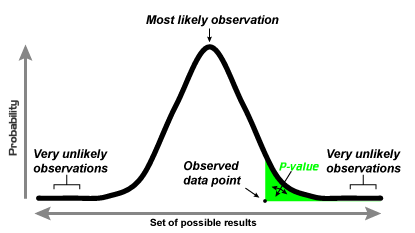
\includegraphics[width=0.6\linewidth]{figures/method/pvalue.png}
\caption{A one-tailed test, showing the p-value as the size of one tail. Credits to \url{https://en.wikipedia.org/wiki/One-_and_two-tailed_tests}}
\label{fig:p-val-one-tailed}
\end{figure}
In hypothesis testing, the initial assumption is that there is no correlation between the predictor and outcome variables in the population. Through statistical tests utilizing collected data, a determination is made as to whether there is enough evidence to reject the null hypothesis in favor of the alternative hypothesis. A two-tailed hypothesis test is designed to show whether the measure is significantly greater than and significantly less than the mean of a population. The two-tailed test gets its name from testing the area under both tails (sides) of a normal distribution. On the other hand, a one-tailed hypothesis test is set up to show that the measure would be higher or lower than the population mean. \autoref{fig:p-val-one-tailed} illustrates a one-tailed test, showing the p-value as the size of one tail. The level of statistical significance, represented by p-values, serves as the benchmark for these tests. The p-value is the likelihood of obtaining the study results by chance if the null hypothesis is true.
\begin{definition}
\label{def:pvalues} 
The p-value is the inverse of the cumulative distribution function of the test statistic. it defines the probability of accepting the alternate hypothesis with a given level of statistical confidence where in fact the null hypothesis is true:
$$ p(ts \geq h) = \int_{h}^{\infty} \phi(x) \,dx $$
where $ts$ is the test statistic of the experiment, $\phi$ is the distribution of the test statistic of the observed experiments, and $h$ is a threshold.
\end{definition}
In other words, the p-value is the likelihood of committing a type I error (false-positive) if one rejects a null hypothesis that is actually true. On the contrary, a type II error (false-negative) occurs if one fails to reject a null hypothesis that is actually false.
The null hypothesis is rejected in favor of the alternative hypothesis if the p-value is less than the established level of statistical significance. 
For example, we can reject the null hypothesis if the p-value is less than $3x10^{-7}$ meaning $> 5\sigma$ confidence in the alternative hypothesis. 
Results with p-values lower than $3x10^{-7}$ can still be false positives every once in $3x10^7$ measures ($\pm$ statistical fluctuations). A metric that considers the number of false positives (or false alarms) per the total number of times the event didn't happen is called \textit{false alarm rate} (FAR). A false alarm rate is also known as the probability of false detection. To not be confused with the false alarm ratio (also abbreviated as FAR), which is the number of false alarms per the total number of warnings or alarms. Regarding hypothesis testing, if P is the probability of committing a type I error (rejecting the null hypothesis when it is actually true) and Q is the probability of making a type II error (failing to reject the null hypothesis when it is actually false), in this study, we prioritize minimizing Q over P to minimize the false positive rate and prevent the system from issuing false science alerts to the scientific community. 

The null hypothesis in this context is represented by the absence of the GRB event in the data. The anomaly score is the test statistic considered in the p-value analysis. To evaluate the p-values, a data set composed of background-only data samples is fed to the autoencoder, and the distribution $\phi$ of the corresponding anomaly scores is computed. Then, the inverse of the cumulative distribution function is evaluated, obtaining a mapping between the test statistics and the p-values. As stated before, a p-value defines the probability of obtaining statistical confidence greater or equal to a threshold $h$ when the null hypothesis is true. 

To reach the desired $5\sigma$ level, about $1e^8$ trials need to be simulated and transformed into sub-sequences fed to the autoencoder to obtain the anomaly scores. The same simulation settings are used to generate the training test for the autoencoder models. Hence, more details about the data set generation for the p-value analysis will be provided in \autoref{ss:training}. There're only two differences concerning the simulation parameters used to generate the training set: the observation time is limited to 100 seconds, and the number of simulated trials is $1e^8$. This process is very computing intensive and has to be repeated several times each time a new model is deployed in production. The latter number is why the simulation script provided by \cite{dipiano2022ctasagsci} has been improved and optimized. As outlined in \autoref{ss:dl3-simulator}, starting from this data set, it is possible to perform different photometry analyses and extract sub-sequences with different lengths. For this reason, a script exploiting batch parallelization with Slurm has been developed to load a trained autoencoder, apply the photometry analysis, generate the sub-sequences, and perform inferences. In particular, each Slurm job takes a batch of photon lists, integrates the photon counts, computes the flux, extracts the time series, scales the data, and performs inference, measuring the anomaly score. In order to guarantee the statistical independence of these measures, from each photon list, only one sub-sequence is generated and given to the autoencoder. This is why the observation time was limited to 100 seconds. The time took to process $1e^7$ trials (about $3.5 TB$ of data), using 100 jobs on 60 Intel(R) Xeon(R) Gold 6240 CPU  cores, was about 48 hours. The computational bottleneck was due to the network filesystem that limited the data transfer from a SATA hard drive. 

In order to find the corresponding p-value for a given sigma level, first of all, we defined the two-tailed probability corresponding to the sigma level of choice. For example, if $sigma=3$, the corresponding two-tailed probability is $p=99.73\%$. The p-value is given by the survival function: $(1-p)=0.0027$. This p-value describes the probability of having a measure outside the  $\pm3\sigma$. Since this use case is constructed on half of a symmetrical distribution, the one-tailed p-value of that probability must be computed. Hence, the previous p-value must be halved, obtaining $(1-p)/2=0.00135$. The p-value is then mapped to a threshold value. On the contrary, if we want to know the sigma level of a particular threshold, we take the corresponding p-value and find the inverse cumulative distribution function relative to that p-value. Again, since the normal distribution is symmetrical, the absolute value is the number of standard deviations rather than  $\pm n\sigma$. if the threshold value is not present in the table, it can be interpolated within the closest two values along with the corresponding p-values interpolation.  

%%%%%%%%%%%%%%%%%%%%%%%%%%%%%%%%%
% QUESTA PARTE E' DA FINIRE
%%%%%%%%%%%%%%%%%%%%%%%%%%%%%%%%%

\section{Inference}
\label{ss:inference}

% Plot predictions not anomalous and anomalous
% SI ottiene MSE
% Si calcola sigma
% Si ripete fino alla fine della timeseries
\autoref{fig:cnn-predictions-itime-5}

\begin{figure}[!htb]
\centering
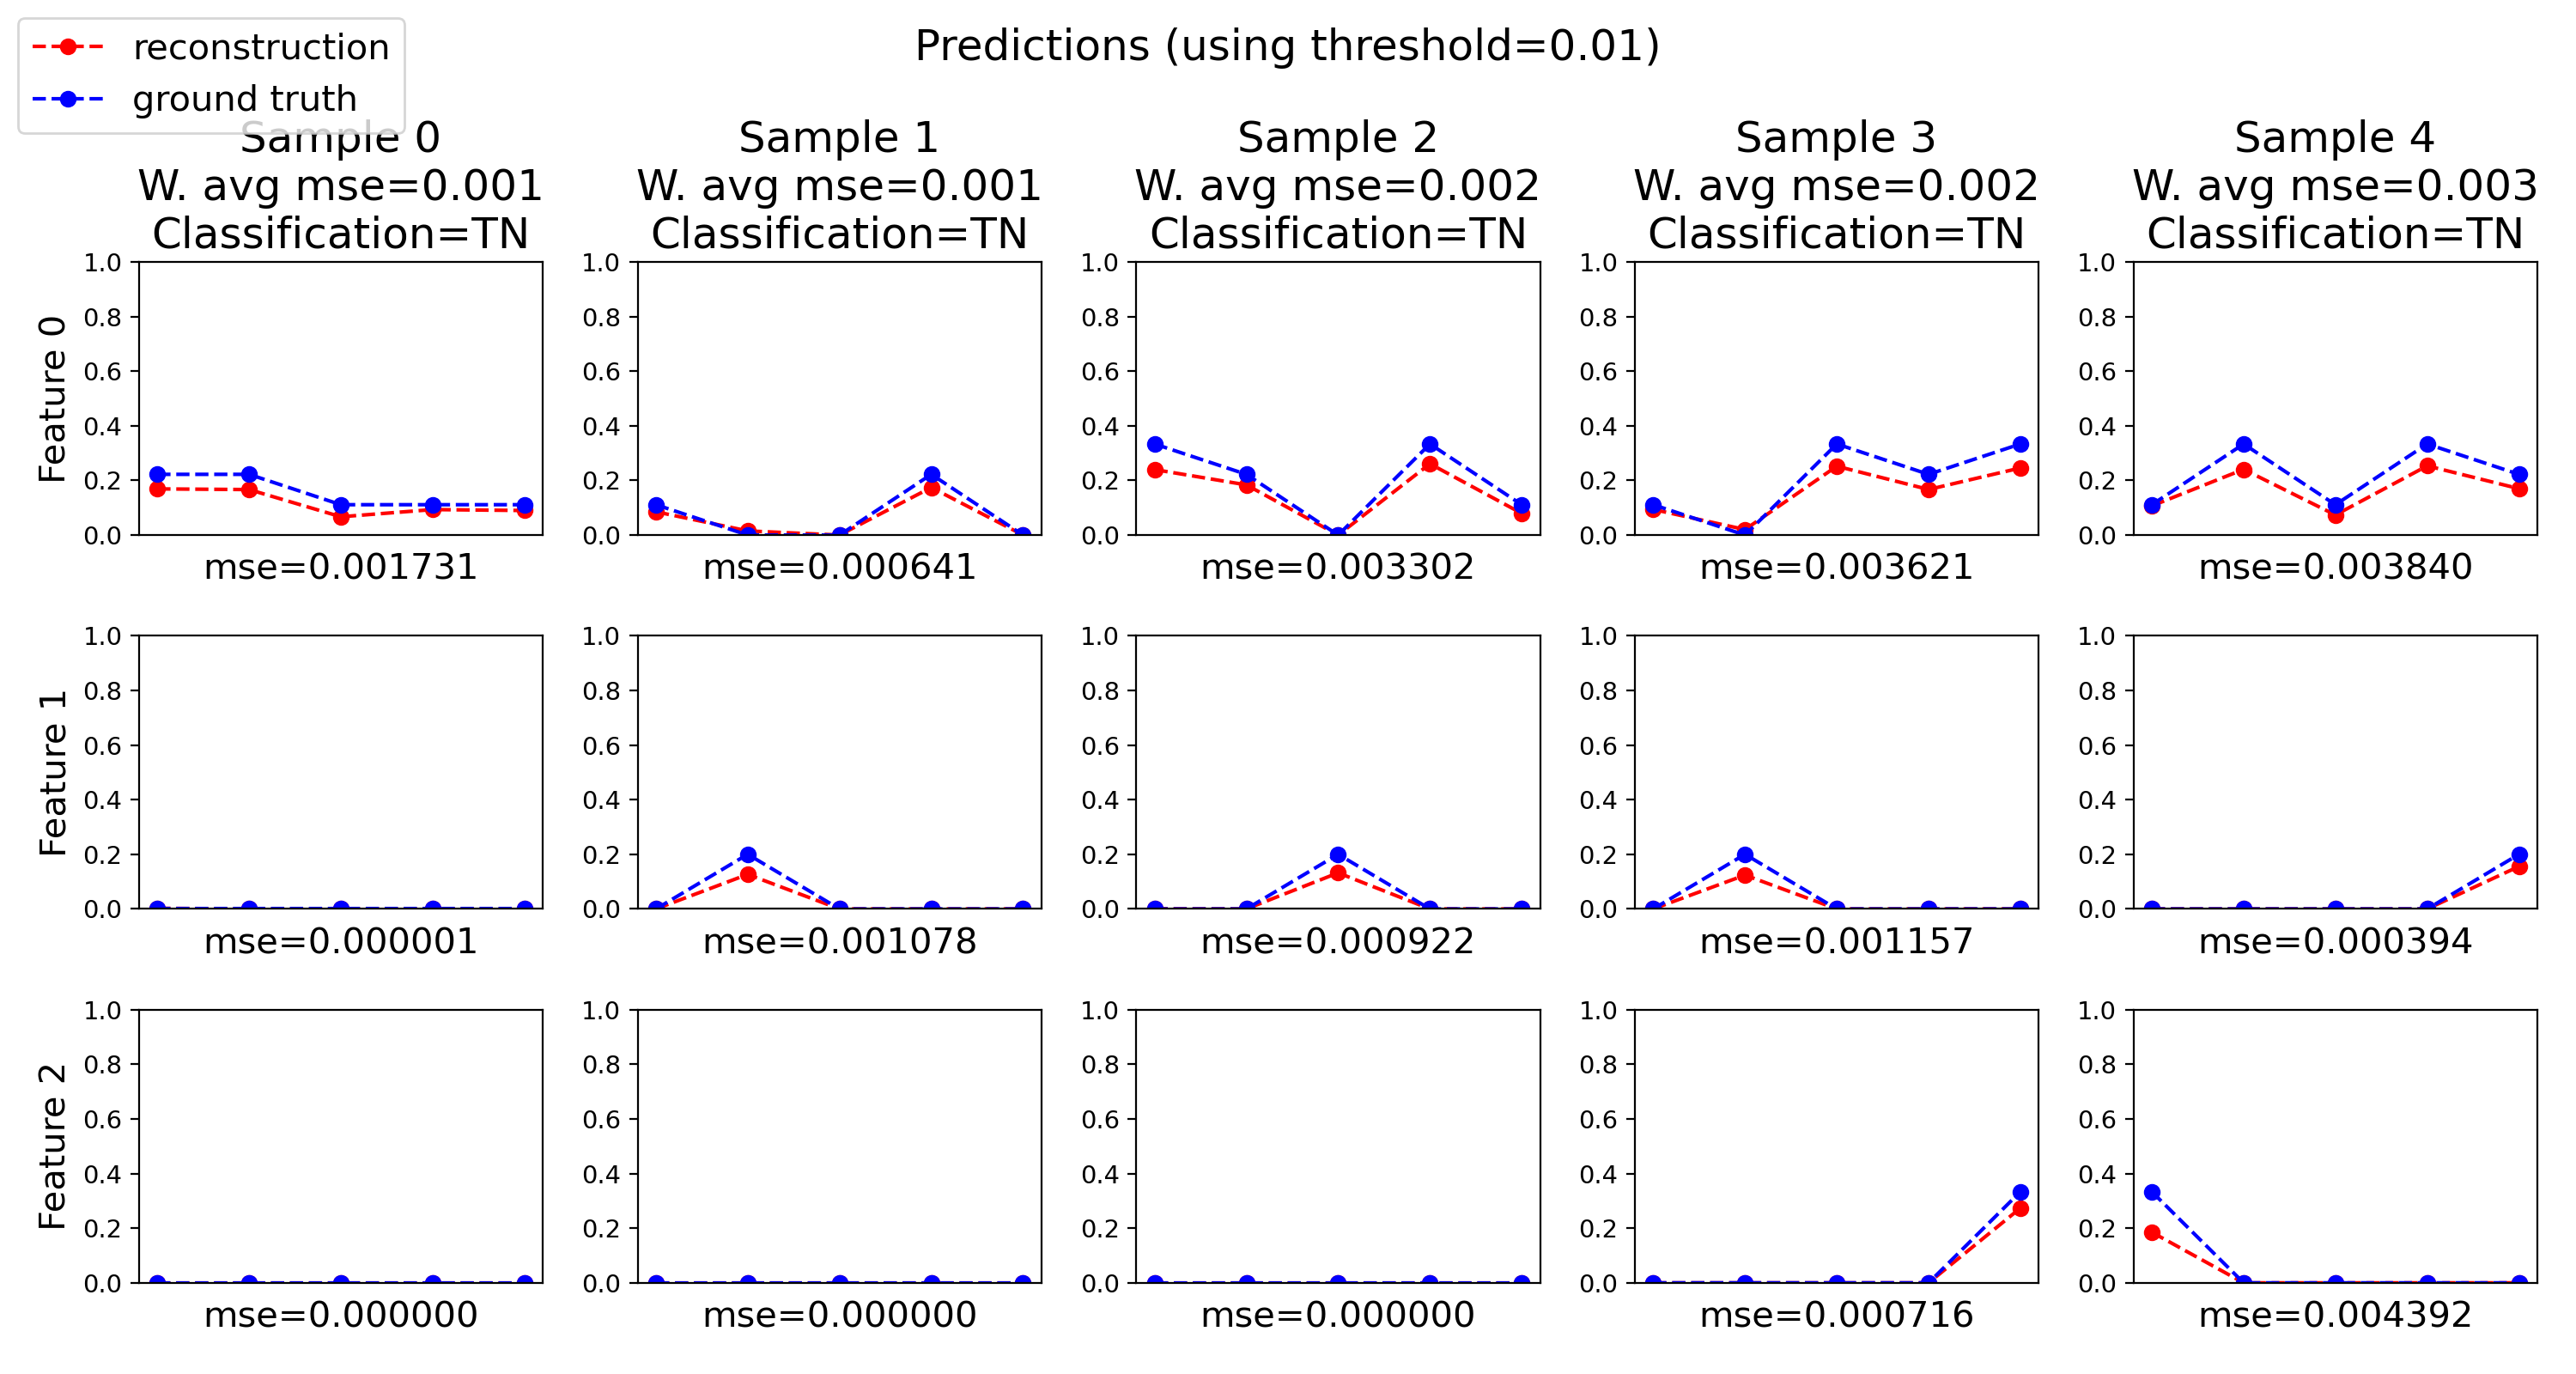
\includegraphics[width=\linewidth]{figures/training/cnn_epoch_5_plot_0_predictions_itime_5.png}
\caption{ }
\label{fig:cnn-predictions-itime-5}
\end{figure}

\begin{figure}[!htb]
\centering
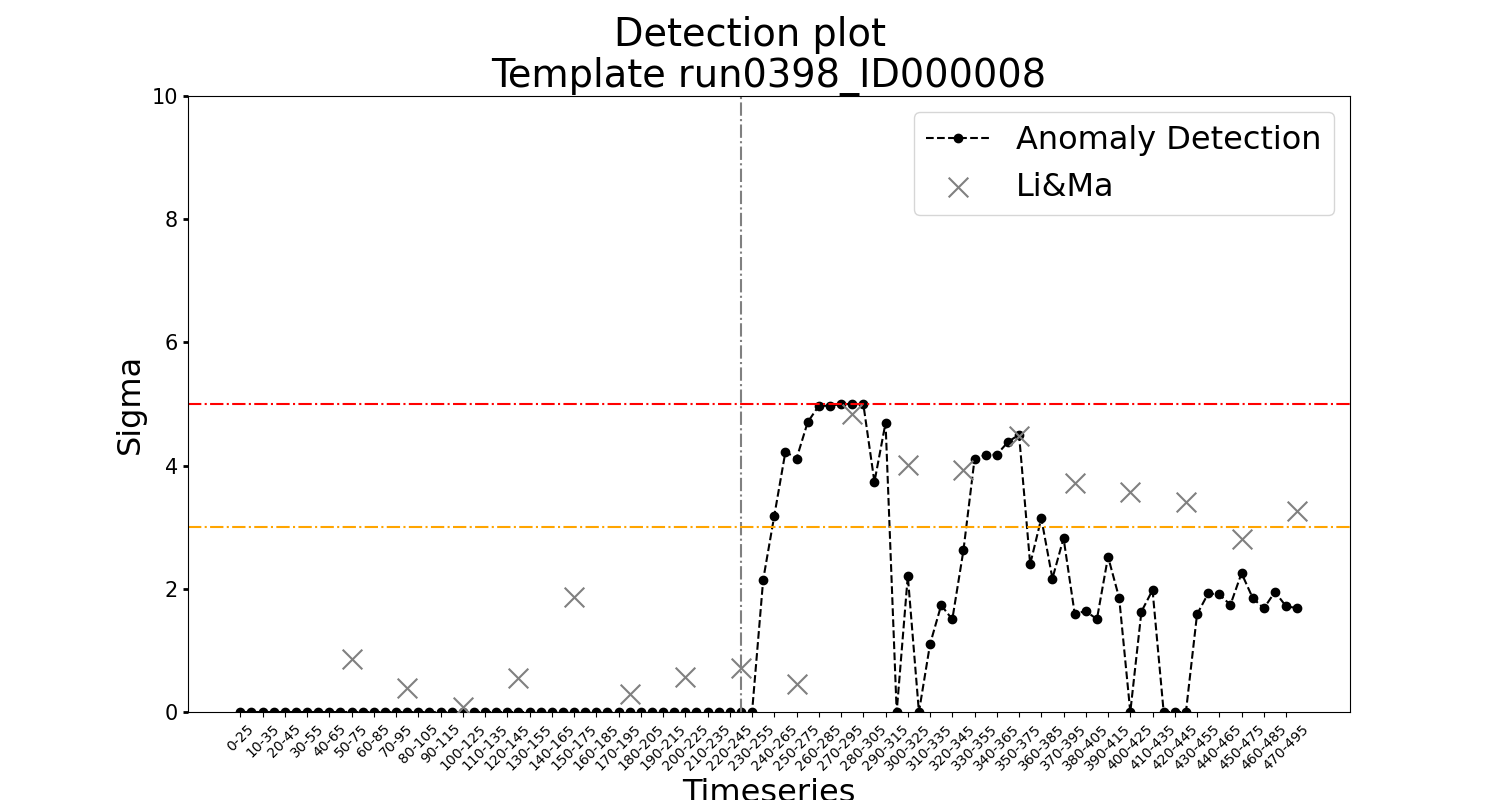
\includegraphics[width=\linewidth]{figures/experiments/detection_plots/detection_plot_run0398_ID000008_testset_e.png}
\caption{ }
\label{fig:detection_plot}
\end{figure}



\section{System design}
\label{s:system-design}

\begin{figure}[!htb]
\centering
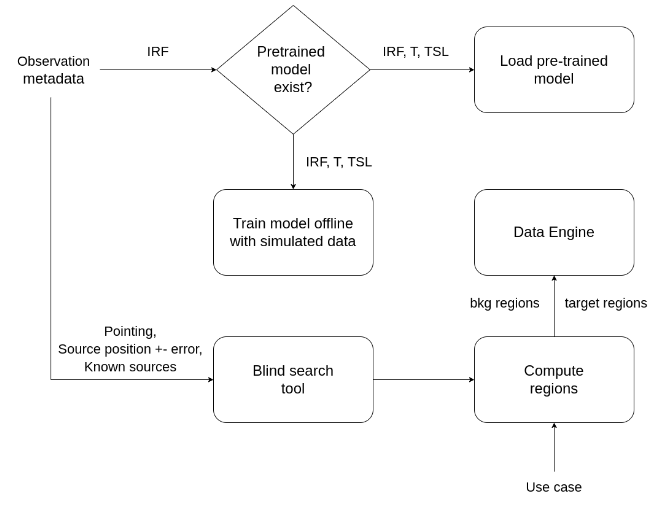
\includegraphics[width=\linewidth]{figures/method/systemdesign1.png}
\caption{ }
\label{fig:system-design-1}
\end{figure}

\section{Non-stationary settings}
\label{s:non-stationary-settings}
During inference, the model will process the real-time data generated by the telescopes during an observation. As explained in \autoref{s:anomaly-detection}, the stationarity property of the stochastic process that generates the data can be invalidated by concept drifts. This can be a significant issue as it can negatively impact the performance of a machine learning model trained under a certain statistical distribution of input data. Neural networks are particularly vulnerable to concept drift, as they rely on the assumption that the data distribution remains constant during training and inference. In the presence of a concept drift, the model makes predictions based on outdated information, leading to decreased accuracy. 





\section{Summary}
The previous chapter proposed a method to address the real-time source detection problem. The contribution described the anomaly detection technique, including the data pipeline for input generation, the investigated deep learning architectures, and the training process. The evaluation of the models was addressed in the experiment setup section. The p-value analysis was described to associate positive classifications with gaussian statistical significance. The potential problems of non-stationary settings during telescope observations and their impact on the proposed system were investigated. 
  \newpage

  \chapter{Results}\label{c:Results}
  \begin{chapabstract}
\small{
This chapter presents the several results experimental measurements of the performance of the Anomaly Detection technique presented in \autoref{s:contribution}.
}\\
\begin{center}
\noindent\makebox[0.8\linewidth]{\rule{0.66\paperwidth}{0.4pt}}
\end{center}
\vspace{1cm}
\end{chapabstract}

\section{Experiments setup}
\label{s:Experiment-Setup}
This chapter presents the results of a study that aimed to develop an anomaly detection technique for addressing the real-time source detection problem in the context of the Cherenkov Telescope Array Observatory (CTAO). As outlined in \autoref{s:contribution}, the proposed anomaly detection technique is based on an autoencoder model. Two autoencoder architectures based on convolutional and recurrent layers have been investigated. The comparison of their performances concerning standard machine learning metrics will be presented in this chapter. A p-value statistical analysis was performed to determine the classification thresholds the models can use to associate $5\sigma$ statistical significances to positive detections. This chapter will also present the results of these analyses. 
This chapter's core focus is to verify if the proposed technique that overcomes the limitations of the standard analyses presented in \autoref{ss:li-ma} and \autoref{ss:ffov-ml} obtains better performances in practice. Key performance indicators (KPIs) have been defined in the context of two scientific use cases: \textit{serendipitous discovery} and \textit{follow-up observations}, introduced in \autoref{s:contribution-1-use-cases}. The results have been compared against the performances of the Li\&Ma analysis technique. The KPIs were first evaluated in the short-term scenario, using an integration time of 5 seconds meaning that each point of the sub-sequences aggregates 5 seconds of data. Furthermore, the same evaluations were repeated in the very short-term scenario, using an integration time of 1 second. The next section will re-introduce the scientific use cases of serendipitous discovery and follow-up observations, highlighting the assumptions and the experiments' setup.

\subsection{Scientific use cases and assumptions}
The serendipitous discoveries use case models the scenario in which the telescopes are observing a certain sky region, and an unexpected event is seen in the field of view. This kind of discovery is possible even though the probability of a serendipitous GRB event appearing in the field of view during an observation is very low. Indeed, telescopes can systematically observe large sky regions, for example, during surveys, increasing the probability of serendipitous discoveries. Such events are scientifically crucial because the overall evolution of the GRB event can be observed from the beginning. To maximize the scientific return, detecting the serendipitous source should be addressed as soon as possible to let other observatories acknowledge the discovery through a science alert broadcasted to the scientific community. By doing so, the same events can be studied with other instruments, exploring different wavelengths or messengers. 
The telescope's field of view (FOV) is larger than the region of interest (ROI). Considering only one ROI, the probability the serendipitous source will appear exactly in its center is even lower. One way to mitigate the problem is to use several ROIs as shown by \autoref{fig:rings}. The problem with this approach is the significant increase in the number of analysis trials, which must be considered as a post-trials probability. In the context of this work, another assumption is made, a blind-search analysis applied in the whole field of view in order to localize candidate sources in the least possible amount of time. One example of blind-search implementation is provided by CTools \cite{Knodlseder_2016}, executing a peak-detection algorithm on smoothed count maps with a localization acceptance threshold above a given significance. It is assumed that the blind-search analysis will always find the region that contains the GRB event in its center for each GRB event considered in the performance analysis. It is also assumed that blind-search will always take a fixed time of 10 seconds to find the region. 

The observatory must not only be the sender of scientific alerts, but it must be capable of receiving and reacting to external ones. The follow-up observation use case models the scenario in which the observatory receives a science alert and changes the pointing of its telescope to a new sky region to detect the event. Several considerations should be made. First of all, the time that passes from the event's start and the taking of the first photon counts, is variable. It depends on two factors: the time to receive the scientific alert and the time the telescopes take to change the pointing. This delay has been considered with four different values: 25, 50, 75, and 100 seconds. After this delay, once the required data is obtained, the analysis techniques can start to perform classifications. Unlike the serendipitous discovery scenario, the evolution of the GRB event cannot be observed from the beginning. The luminosity of a GRB event tends to decrease over time, increasing the difficulty of detection. Another factor to consider is the localization error on the position of the source provided by the received scientific alert. This error can be smaller than the field of view or much larger, as in the case of a gravitational-wave alert. The latter case would require multiple observations performed with a tiling strategy \cite{di2020detection}, but this is outside of the scope of this work. If the localization error within the field of view must be covered by multiple ROIs, the blind-search approach used in the serendipitous scenario will also be considered here.   

 
\subsection{Test set generation}
\label{s:Experiment-Data}
The test set used for the performance evaluation of the proposed anomaly detection method is a supervised data set containing two classes of samples. The first class of samples has been generated considering the background model in the simulations. The second class of samples has been generated considering the background and source models in the simulations. The templates used for the Gamma-Ray Bursts (GRBs) simulations were taken from the POSyTIVE catalog. The mock GRB population used by POSyTIVE is calibrated using a 40-year dataset of multi-wavelength GRB observations \cite{Bernardini_2019}, providing about 20 thousand GRB templates of known events.
As stated in \autoref{s:Gamma-Ray-Bursts}, GRBs are characterized by several key properties, including duration and peak flux. The latter measures the maximum energy level emitted by the event. It is usually measured in units of $erg/s/cm^2$ and is one of the most important parameters for characterizing the luminosity of a GRB. GRBs can have a wide range of peak fluxes, from as low as $10^-9 erg/s/cm^2$ to as high as $10^-5 erg/s/cm^2$, depending on the distance and its intrinsic properties. If the luminosity is too low, the GRB event will be indistinguishable from the background noise. For this reason, but also computational resource limitations, only a subset of the entire catalog has been simulated. 
The mean of the background level has been considered a threshold to limit the number of simulations. The test set has been generated simulating all the templates whose peak flux is greater or equal to the background level mean minus $1\sigma$, to account for the background fluctuations. Figure~\ref{f:exp-max-flux-distribution-E} shows the distribution of the peak flux of each GRB template and highlights the selected set. As explained in \autoref{dl3-simulator}, the simulation tool generates a photons list, i.e., a list of photons whose energy and arrival direction are reconstructed. Only the GRB afterglow model has been simulated since the prompt models were not available at the time of writing. The simulation tool has been used to generate one simulated trial for each selected template. The resulting test set contains 419 trials with a peak flux in the interval $[2.6785e-10, \infty]$.
\begin{figure}[!htb]
\centering
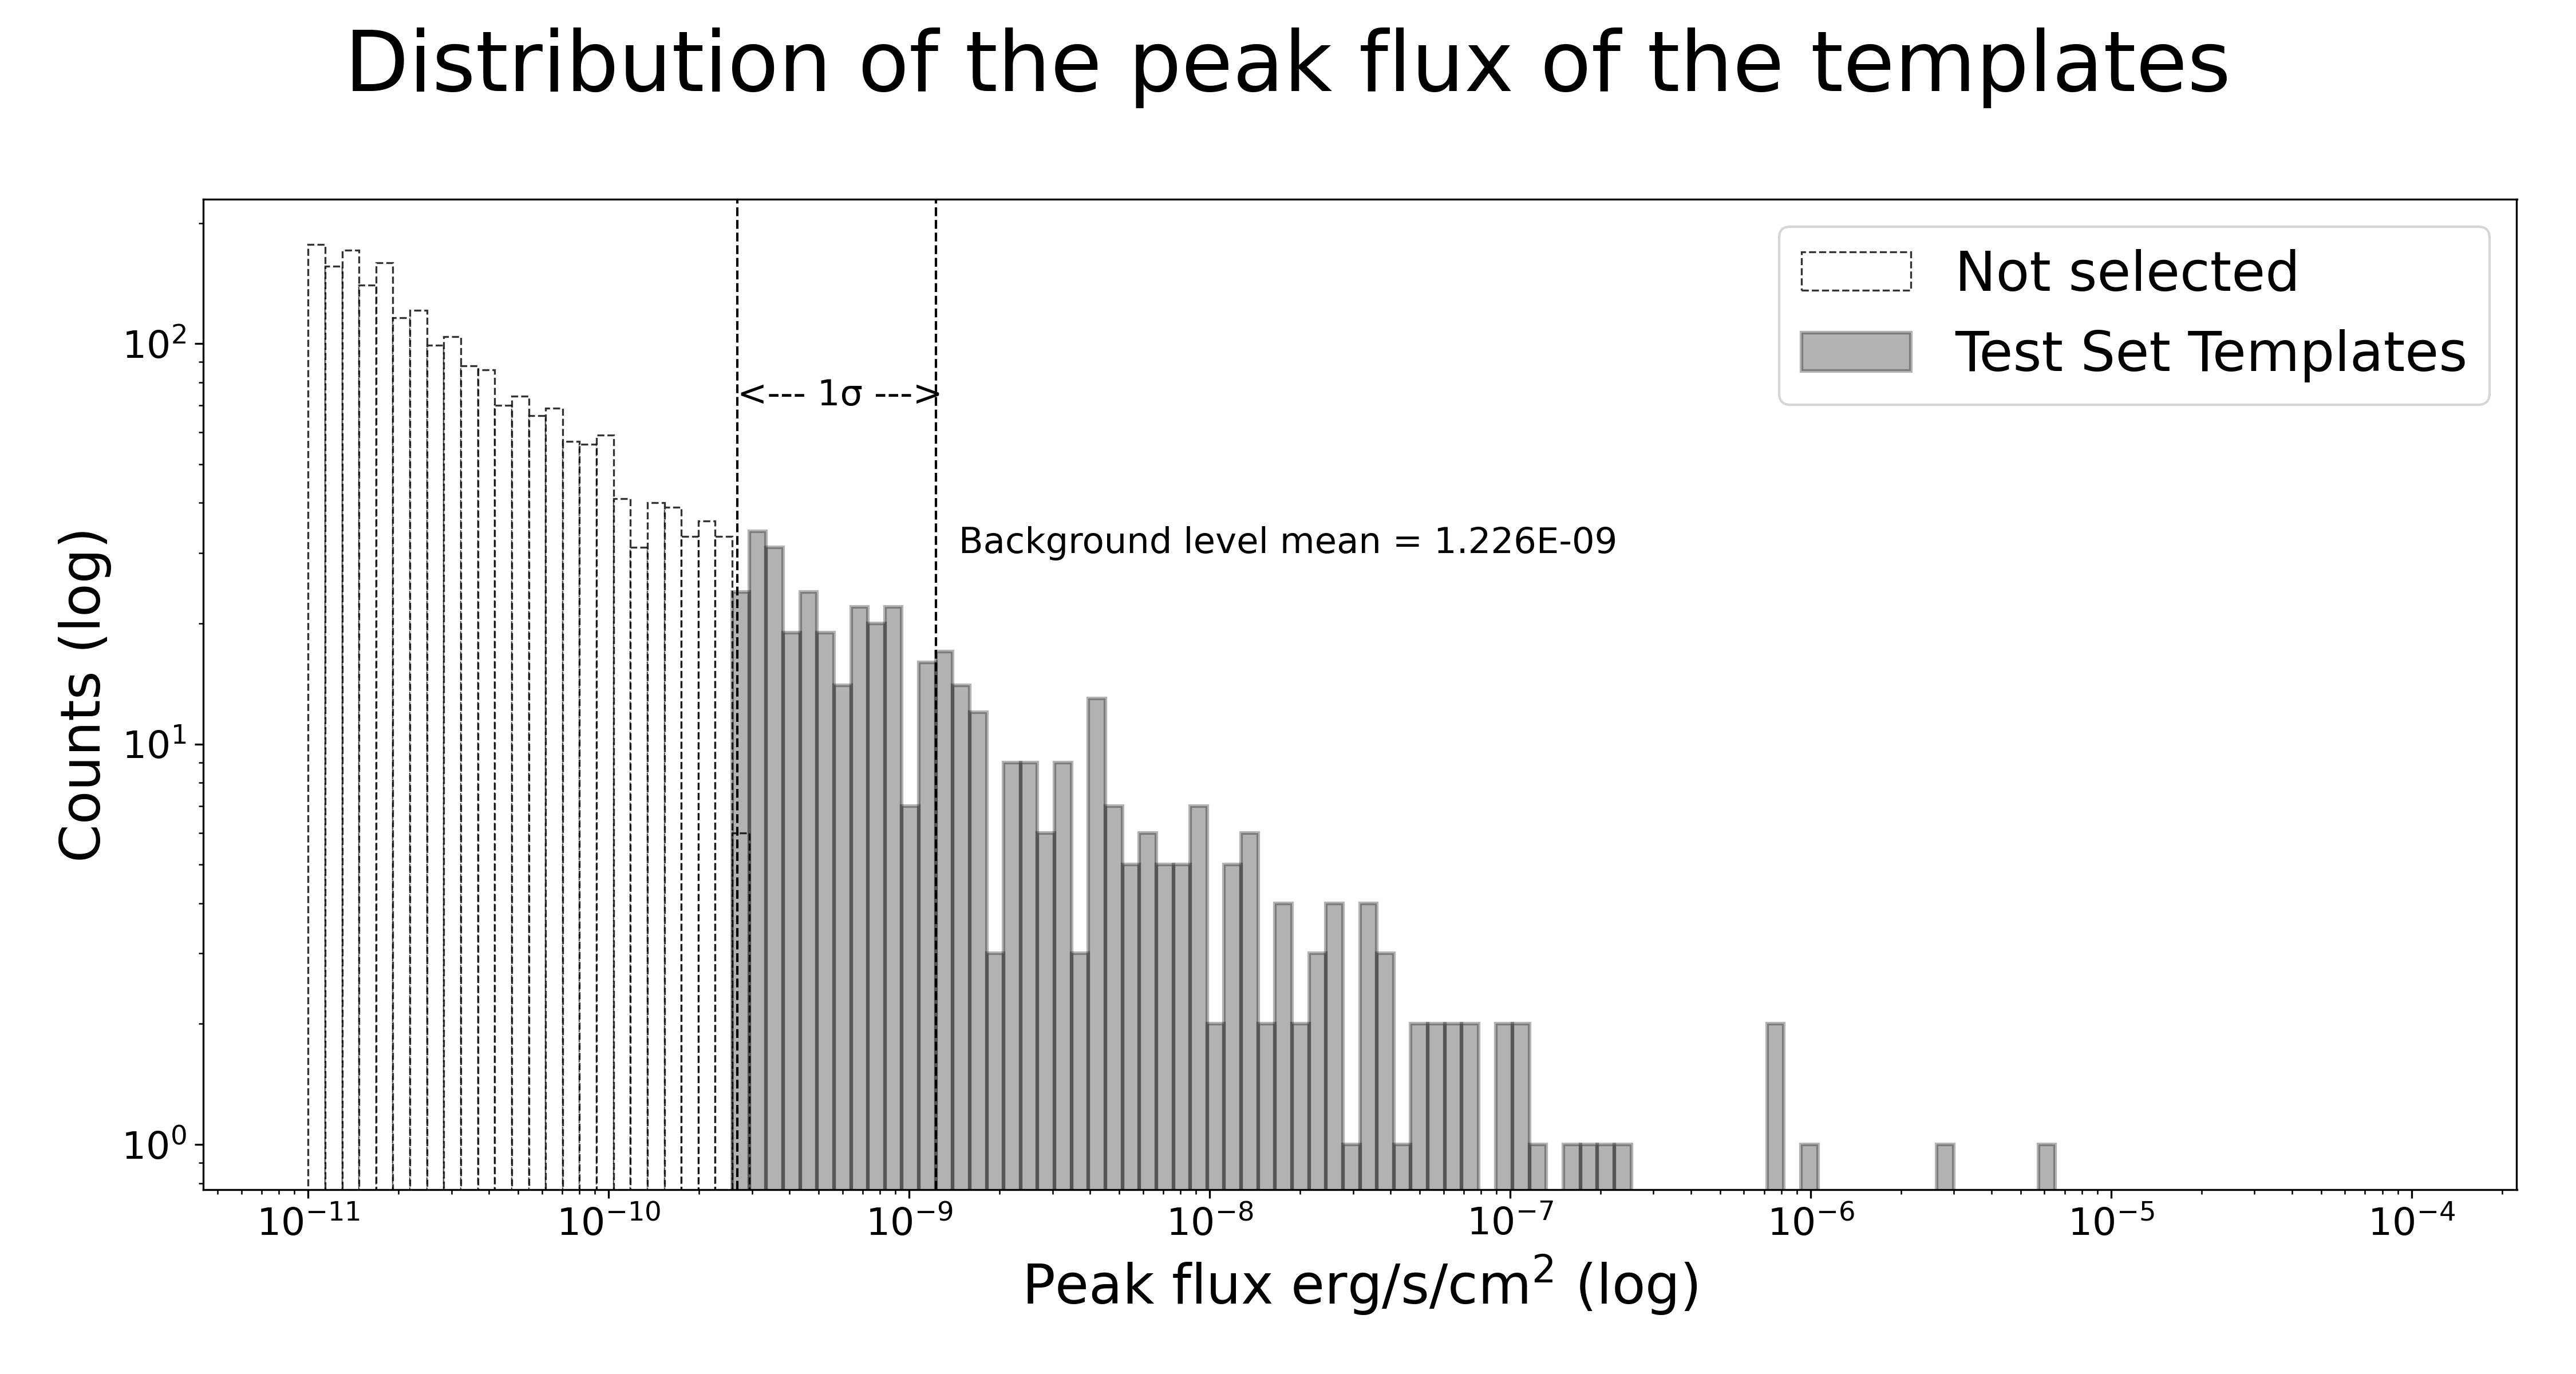
\includegraphics[width=1\textwidth]{figures/experiments/templates_max_flux_distributions.png}
\captionsetup{width=0.9\linewidth}
\caption{The distribution of the peak flux for each GRB template. The selected templates are 419, and their peak fluxes are within the $[2.6785e-10, \infty]$ range.}
\label{f:exp-max-flux-distribution-E}
\end{figure}
The simulation time is limited to 500 seconds because we are interested in detecting the event as soon as possible. The trigger time that defines the start of the GRB event is fixed and equal to 250 seconds. The instrument response function (IRF) is the same used for generating the training set, which models the response of an LST-1 telescope located in the northern hemisphere site, observing for 5 hours at $40^{\circ}$ zenith angle.
As described in \autoref{ss:integrator-module}, the photons lists must be integrated in space, time, and energy to generate the multi-variate time series of flux measurements. The integration time is set to 5 seconds to evaluate the performances of the techniques in the short-term scenario and 1 second for the very short-term scenario. The integration process generates time series of 100 (short-term scenario) and 500 (very short-term scenario) flux measurements. Finally, as described in \autoref{ss:extractor}, the time series extractor module extracts sub-sequences from the generated time series. The length of the sub-sequences is fixed and set to 5 points, the same setting used to generate the data to train the auto-encoder. The stride parameter is set to 1 because the anomaly detection technique can use overlapping temporal bins, drastically reducing the time the model waits for data during the online inference. In contrast, the Li\&Ma technique must use temporal bins that are statistically independent. Finally, each sub-sequence is associated with a label. A sub-sequence is labeled as anomalous if at least one of its points exceeds the trigger time threshold that defines the start of the GRB event. For the short-term scenario (integration time = 5 seconds), the number of generated test samples is 40224, of which 20531 are labeled anomalous. For the very short-term scenario (integration time = 1 second), the number of test samples is 207824, of which 104331 are labeled anomalous.


\FloatBarrier
\section{P-value analysis results}
\label{s:p-values-results}
As outlined in \autoref{ss:p-values}, the p-value analysis is used to obtain the threshold $\tau$ to classify the samples as anomalies with a certain $\sigma$ level or, on the contrary, to associate with each anomaly score a statistical confidence level (of a positive classification). Four p-value analyses have been performed, one for each autoencoder model (convolutional and recurrent) in the short-term and very short-term settings. The models performed inferences on $1e^8$ background-only samples, and the distributions of the anomaly score (weighted mean squared error) have been computed. Then, the inverse cumulative of the distribution function was evaluated, and the mapping between the y-axis (p-values) and the x-axis (anomaly scores) was written on disk. 
\begin{figure}[!htb]
    \centering
    \begin{minipage}{0.5\textwidth}
        \centering
        \includesvg[width=\linewidth]{figures/experiments/p_val/model_1_ts.svg}
    \end{minipage}%
    \begin{minipage}{0.5\textwidth}
       \centering
       \includesvg[width=\linewidth]{figures/experiments/p_val/model_1_pvalues.svg}
    \end{minipage}
    \captionsetup{width=0.9\linewidth}
    \caption{TS distribution and p-values for the autoencoder with recurrent layers in the short-term scenario (integration time = 5 seconds).}
    \label{fig:ts-distribution-and-p-values-rnn-it-5}
\end{figure}

\begin{table}[!htb]
\centering
\begin{tabular}{|p{3cm}|p{3cm}|p{3cm}|p{3cm}|}
\hline
\multicolumn{4}{|c|}{p-values} \\
\hline
Threshold & p-value & $\pm$ error &  Sigma \\
\hline
0.003171 &  1.283972e-01 &  1.201785e-04 &  1.134 \\
0.003751 &  6.115264e-02 &  8.293861e-05 &  1.545 \\
0.004476 &  2.277199e-02 &  5.061155e-05 &  2.000 \\
0.005492 &  5.323285e-03 &  2.447028e-05 &  2.554 \\
0.006507 &  1.228234e-03 &  1.175411e-05 &  3.029 \\
0.007667 &  2.312711e-04 &  5.100465e-06 &  3.502 \\
0.009118 &  3.149606e-05 &  1.882250e-06 &  4.001 \\
0.010859 &  3.262092e-06 &  6.057553e-07 &  4.509 \\
0.013760 &  4.499438e-07 &  2.249719e-07 &  4.912 \\
0.013905 &  2.249719e-07 &  1.590791e-07 &  5.047 \\
\hline
\end{tabular}
\caption{An example of p-value analysis for the autoencoder with recurrent layers in the short-term scenario (integration time = 5 seconds). The table shows a subset of all the rows. Only the threshold values corresponding to predefined sigma levels are shown.}
\label{tab:p-value-table-rnn-itime-5}
\end{table}
The visualization tool of \cite{dipiano2022ctasagsci} has been used to compute the plots shown in \autoref{fig:ts-distribution-and-p-values-rnn-it-5}. The figure shows the p-value analysis results for the autoencoder with recurrent layers in the short-term scenario. The left panel  shows the test statistic distribution, and the right panel shows the corresponding p-values. \autoref{tab:p-value-table-rnn-itime-5} shows the actual values of the anomaly score - sigma level mapping. The number of rows of the table was limited to only certain levels of sigma. \autoref{s:appendix-a} lists the p-value analysis results for each model and analysis setting. 

 


\section{Comparison of the autoencoder architecures}
\label{s:Acc-Fpr}
As described in Section \autoref{s:contribution}, the proposed anomaly detection technique utilizes an autoencoder model. Both convolutional and recurrent layer-based architectures for autoencoders have been examined. The chapter will compare their performances using standard machine learning metrics. The accuracy, precision, recall, and false positive rate metrics express the percentage of the time series correctly classified, what proportion of positive identifications was actually correct, what proportion of actual positives was identified correctly, and what proportion of the actual negative events were wrongly categorized as positive. While precision measures the probability of a sample classified as positive to be an actual positive sample, the false positive rate measures the ratio of false positives within the negative samples. The accuracy, precision, and recall values computed with different thresholds can help understand the evolution of trade-offs between the number of false positive and false negative classifications. \autoref{fig:rnn-metrics-itime-5} shows the accuracy, precision, and recall curves for the autoencoder model with recurrent layers in the short-term settings (integration time = 5). 
\begin{figure}[!htb]
    \centering
    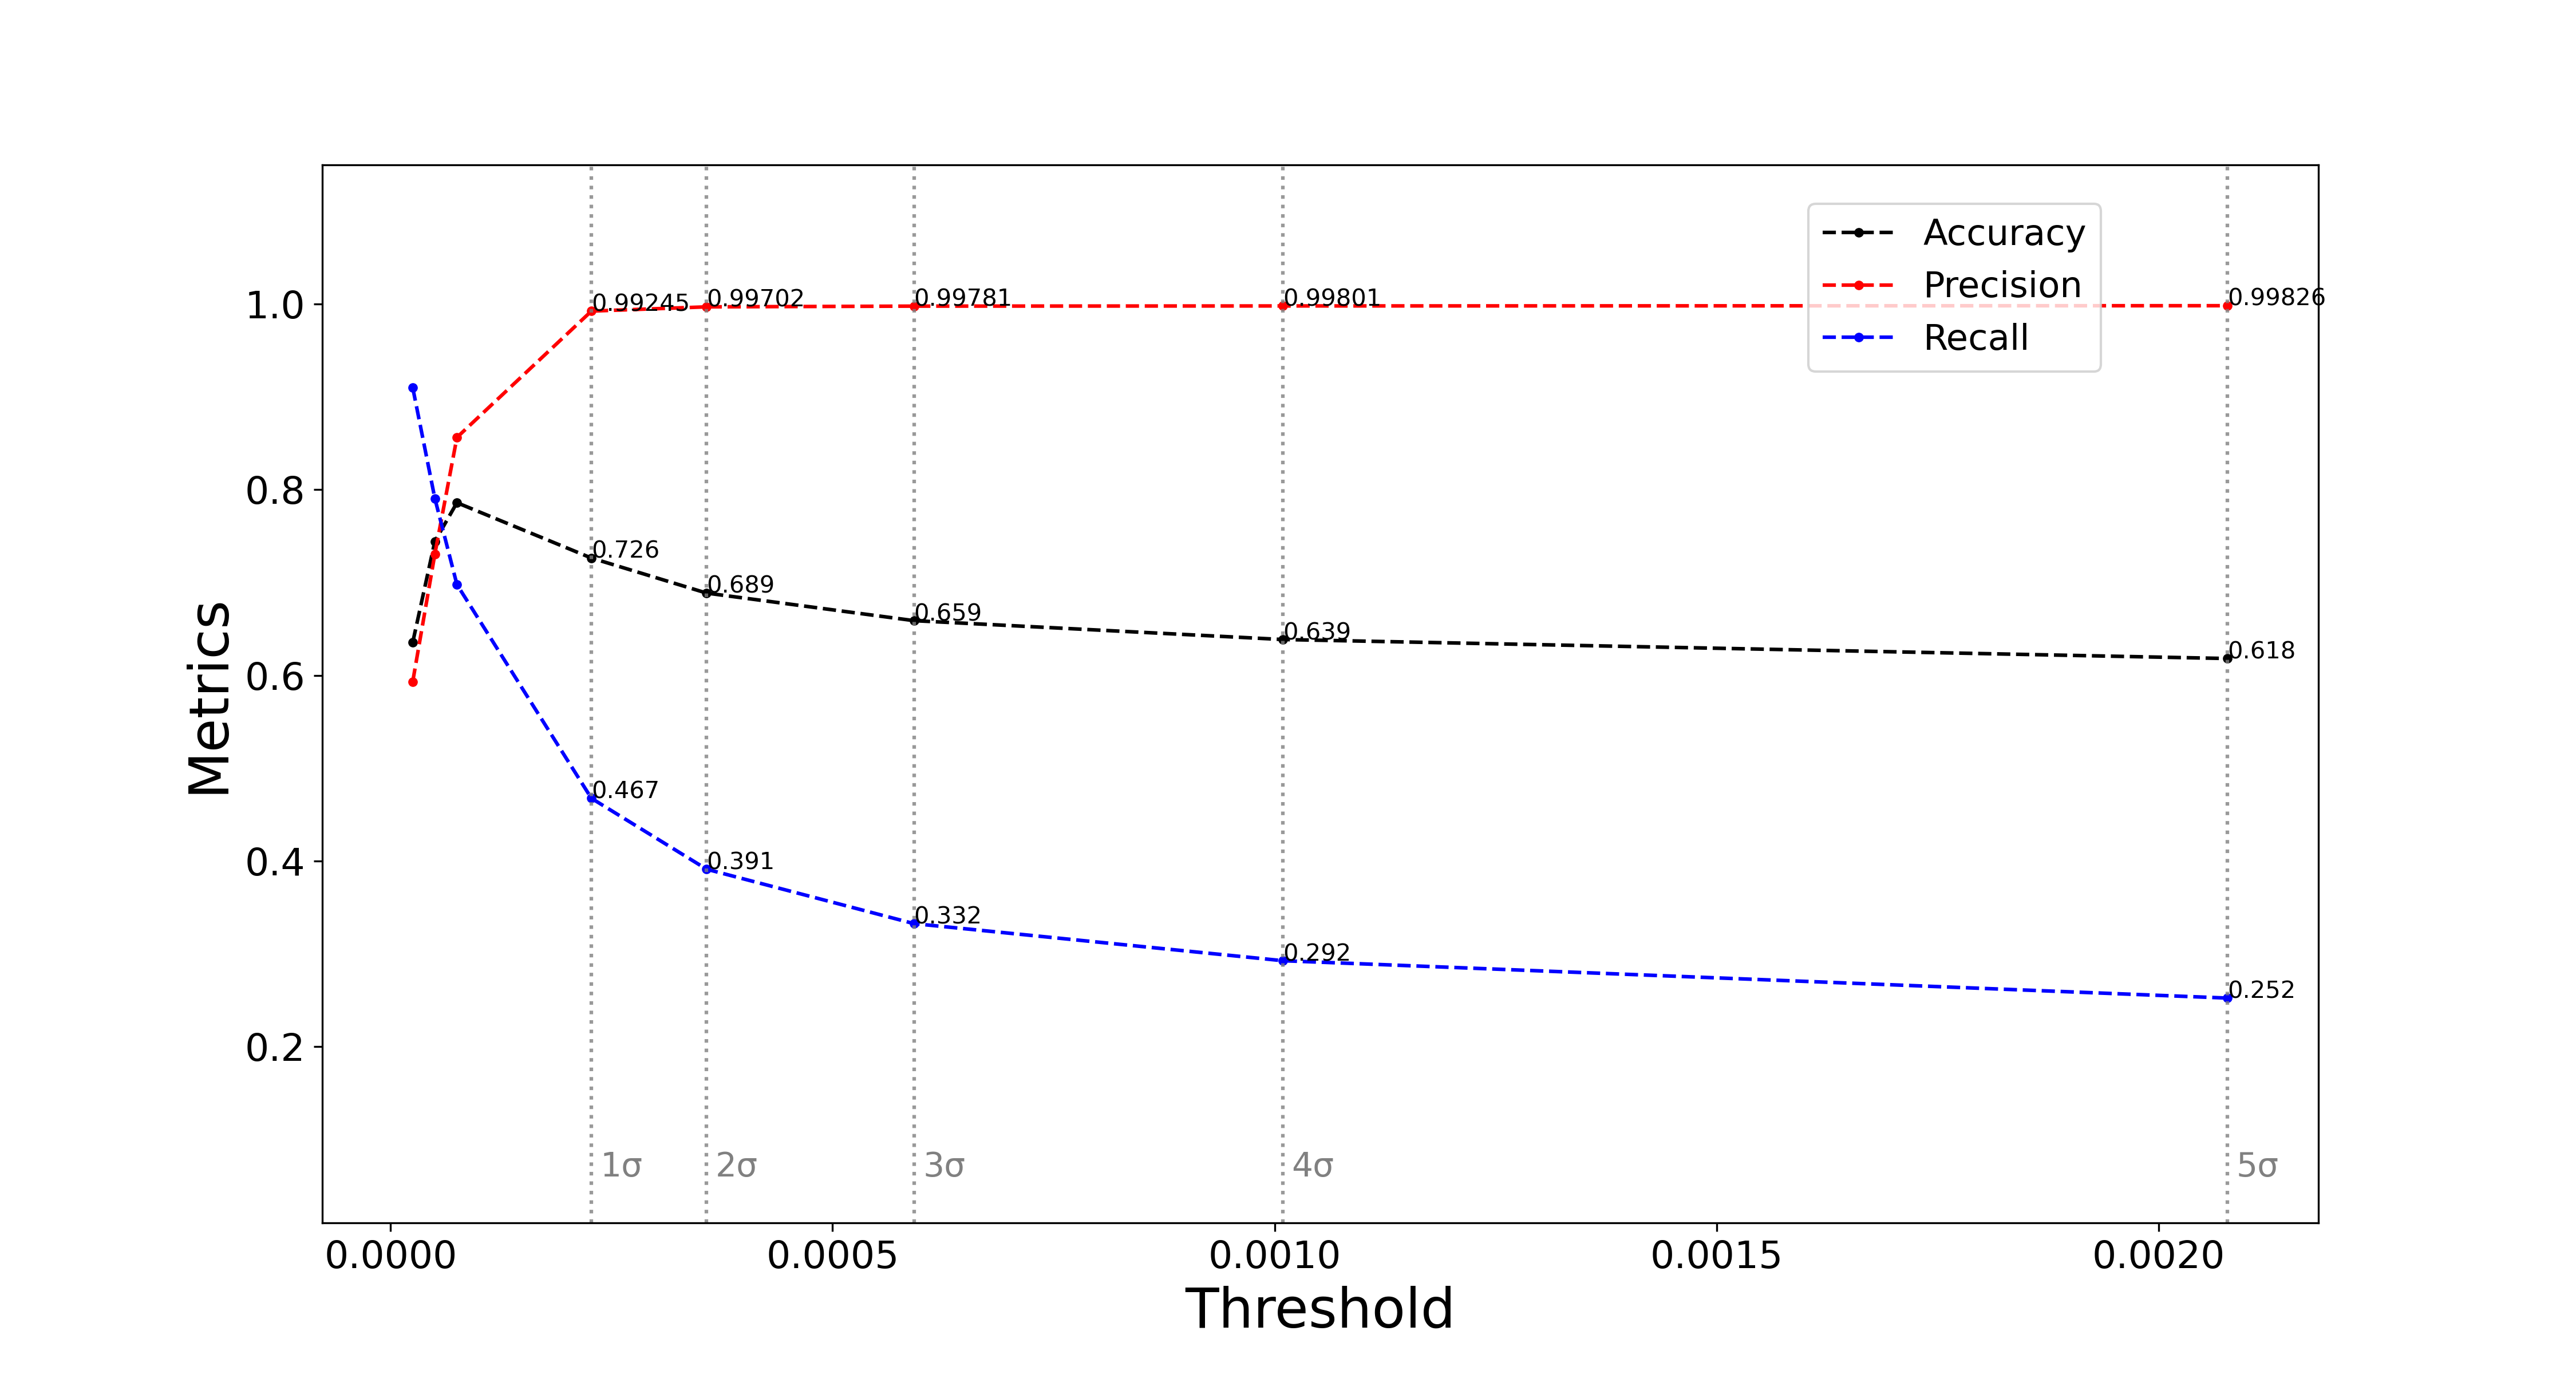
\includegraphics[width=\linewidth]{figures/experiments/metrics/rnn_metrics_test_set_all_itime_5.png}
    \captionsetup{width=0.9\linewidth}
    \caption{Accuracy, precision, and recall curves for the autoencoder model with recurrent layers in the short-term settings (integration time = 5).}
    \label{fig:rnn-metrics-itime-5}
\end{figure}
\autoref{tab:standard-metrics-itime-5} and \autoref{tab:standard-metrics-itime-1} show the actual values of accuracy, precision, recall, and false positive rate computed using the $5\sigma$ threshold, for both architectures and short-term settings. The autoencoder with recurrent layers obtained better accuracy and recall in both scenarios. At the same time, autoencoder with convolutional layers is less precise but has a better false positive rate. 
\begin{table}[!htb]
\centering
\begin{tabular}{|c|c|c|c|c|}
    \hline
    Model & Accuracy & Precision & Recall & False Positive Rate \\ 
    \hline
    RNN & $61.81\%$ & $99.83\%$ & $25.22\%$ & $0.17\%$ \\
    CNN & $59.96\%$ & $99.86\%$ & $21.58\%$ & $0.13\%$ \\
    \hline
    \end{tabular}
\caption{Standard metrics in the short-term settings (integration time = 5), using the $5\sigma$ threshold. The number of test samples is 40224, of which 20531 are anomalous.}
\label{tab:standard-metrics-itime-5}
\vspace{1cm}
\centering
\begin{tabular}{|c|c|c|c|c|}
    \hline
    Model & Accuracy & Precision & Recall & False Positive Rate \\ 
    \hline
    RNN & $57.05\%$ & $99.97\%$ & $14.46\%$ & $0.033\%$ \\
    CNN & $55.58\%$ & $99.98\%$ & $11.52\%$ & $0.016\%$ \\
    \hline
\end{tabular}
\caption{Standard metrics in the very short-term settings (integration time = 1), using the $5\sigma$ threshold. The number of test samples is 207824, of which 104331 are anomalous.}
\label{tab:standard-metrics-itime-1}
\end{table}
\autoref{s:appendix-b} presents the same metrics for each model and analysis setting. 


\FloatBarrier
\section{Evaluation of the proposed technique against Li\&Ma}

\FloatBarrier
\subsection{Key performance indicators}
The first key performance indicator is the cumulative number of $5\sigma$ detections. This metric evaluates the robustness of the techniques. As outlined in \autoref{s:Experiment-Data}, the data set for testing is composed of 419 simulated GRB events. The number of $5\sigma$ detections is evaluated for each time bin whose time span depends on the integration time and the length of the sub-sequences. This number is cumulated for the following time bins. 

For the reasons stated in the previous section, evaluating how fast the technique is to issue $5\sigma$ detections is crucial. Hence the second key performance indicator represents the average time to perform detections. This metric is called \textit{Detection Delay} (DD) and is evaluated as follows. For each time bin, the number of seconds between the start of the GRB event ($t_{grb}=250s$) and the detection time, is computed. This delay ($d_{tb}$) is the same for each detection performed in a time bin. For example, if the autoencoder model performs a detection in time bin $[230-255]$, the delay ($d_{[230-255]}$) is equal to 5 seconds ($255-250$). The delay is computed for each time bin. Then, a weighted average is evaluated, considering the number of the detections in common to the two techniques within the time bins, from $[245-250]$ to $tb_{max}$. Considering the short-term scenario, the detection delay (DD) is defined as:
\begin{equation}
    DD = \frac{1}{tcd} \sum_{tb=[245-250]}^{tb_{max}} w_{tb}*d_{tb}
\end{equation}
Where $tcd$ is the total number of detections in common to the two methods, $w_{tb}$ represents the number of detections made in a particular time bin, and $d_i$ is the delay expressed as the difference between $tb$ and the time bin of the start of the GRB event ($t_{grb}=250s$). 

\FloatBarrier
\subsection{Serendipitous discovery results}
\label{s:Serendipitous-Discoveries-Results}
In the serendipitous discovery scenario, the telescopes observe a certain sky region, and an unexpected event is detected in the field of view. The telescope's field of view (FOV) is larger than the region of interest (ROI). This study assumes a blind-search analysis applied to the whole field of view to select the ROI. In particular, it is assumed that the blind-search analysis will always find the ROI that contains the GRB event in its center and will take a fixed time of 10 seconds to complete.

\FloatBarrier
\subsubsection{Short-term scenario}
\label{s:Serendipitous-Discoveries-Results-Short-Term}
\autoref{f:serendipitous-discoveries-itime-5} shows the cumulative number of detections performed by the anomaly detection and Li\&Ma techniques for each temporal bin in the short-term scenario (integration time = 5 seconds). The x-axis holds each temporal bin. The y-axis holds the cumulative number of detections among all the GRB events.  The vertical dashed line corresponds to the start of the GRB event. The grey area represents the application of the blind-search algorithm, so even if the series start at bin $[225-250]$, only the points outside the grey area must be considered.
\begin{figure}[!ht]
\centering
\includesvg[width=1\textwidth]{figures/experiments/results/serendipitous_discoveries_time_5.svg}
\captionsetup{width=0.9\linewidth}
\caption{The cumulative number of detections of anomaly detection and Li\&Ma techniques for each temporal bin in the short-term scenario (integration time = 5 seconds). The x-axis holds each temporal bin. The y-axis holds the cumulative number of detections among all the GRB events. The vertical dashed line corresponds to the start of the GRB event. The grey area represents the application of the blind-search algorithm.}
\label{f:serendipitous-discoveries-itime-5}
\end{figure}
The figure shows the robustness of the Li\&Ma technique, detecting at the end of the observation more GRBs than the anomaly detection technique. However, we are interested in the first part of the observation since detections must be performed as soon as possible. The anomaly detection technique can be applied after each $T=5$ seconds of new data. In contrast, Li\&Ma is limited by statistical independence assumption and can be applied only for temporal bins that do not overlap. To quantify how faster the anomaly detection technique is concerning Li\&Ma, \autoref{tab:dd-itime-5} shows the DD metric. The first temporal bin considered in the table starts when the blind-search algorithm ends. The next temporal bins are the ones in which Li\&Ma has applied. To be fairer in the comparison against Li\&Ma, \autoref{tab:dd-itime-5-common} reports the same metrics but considers only the same detections performed by both anomaly detection and Li\&Ma techniques. The tables prove the ability of the anomaly detection technique to perform faster detections with respect to Li\&Ma.


 
\begin{table}[!ht]
\centering
\begin{tabular}{|c|cc|cc|cc|} 
\hline
\multicolumn{7}{|c|}{\textbf{Detection delay} (common detections)} \\ 
\hline
\multicolumn{1}{|c|}{Temporal bins} & \multicolumn{2}{c|}{CNN} & \multicolumn{2}{c|}{RNN} & \multicolumn{2}{c|}{Li\&Ma} \\ 
\hline
250-275 &  6.86 &  $\pm$5.41 &  6.37 &  $\pm$5.57 & 15.00 &  $\pm$0 \\
275-300 & 10.78 &  $\pm$9.25 & 12.04 & $\pm$11.56 & 21.28 & $\pm$10.87 \\
300-325 & 14.28 & $\pm$13.69 & 15.98 & $\pm$15.58 & 24.87 & $\pm$14.6 \\
325-350 & 17.02 & $\pm$17.31 & 18.87 & $\pm$18.75 & 27.64 & $\pm$17.9 \\
350-375 & 18.98 & $\pm$19.88 & 21.31 & $\pm$21.79 & 29.59 & $\pm$20.25 \\
\hline
\end{tabular}
\caption{Detection delay (in seconds) for serendipitous discoveries in the short-term scenario (integration time = 5 seconds) with common detections.}
\label{tab:dd-itime-5-common}
\end{table}






\FloatBarrier
\subsubsection{Very short-term scenario}
\label{s:Serendipitous-Discoveries-Results-Very-Short-Term}
The same metrics are evaluated again in the very short-term scenario, with an integration time equal to 1 second. In this scenario, the number of photon counts is further reduced, often exceeding the lower bounds of the Li\&Ma technique (equal to 10), limiting its applicability. In contrast, it reduces the time both techniques need to wait for new data: from 5 to 1 second. Each second, a new flux data measurement is available, and a new sub-sequence is ready for analysis. 
\autoref{f:serendipitous-discoveries-itime-1} shows that the number of detections performed by the anomaly detection technique with recurrent layers is always greater than Li\&Ma's one, proving greater robustness in this extreme scenario. As said before, the Li\&Ma is not always applicable due to its limitation of requiring at least 10 photon counts. The reduced number of photon counts also negatively affects the performance of the anomaly detection technique. Concerning the detection delay, \autoref{tab:dd-itime-1} and \autoref{tab:dd-itime-1-common} show that, even in the very short-term scenario, the anomaly detection technique is faster with respect to Li\&Ma.

\begin{figure}[!ht]
\centering
\includesvg[width=1\textwidth]{figures/experiments/results/serendipitous_discoveries_time_1.svg}
\captionsetup{width=0.9\linewidth}
\caption{The cumulative number of detections of anomaly detection and Li\&Ma techniques for each temporal bin in the very short-term scenario (integration time = 1 seconds). The x-axis holds each temporal bin. The y-axis holds the cumulative number of detections among all the GRB events. The vertical dashed line corresponds to the start of the GRB event. The grey area represents the application of the blind-search algorithm.}
\label{f:serendipitous-discoveries-itime-1}
\end{figure}

 
\begin{table}[!ht]
\centering
\begin{tabular}{|c|cc|cc|cc|} 
\hline
\multicolumn{7}{|c|}{\textbf{Detection delay} (common detections)} \\ 
\hline
\multicolumn{1}{|c|}{Temporal bins} & \multicolumn{2}{c|}{RNN} & \multicolumn{2}{c|}{CNN} & \multicolumn{2}{c|}{Li\&Ma} \\ 
\hline
280-285 & 10.11 &  $\pm$7.46 & 11.04 &  $\pm$7.54  & 11.57 &  $\pm$8.46\\
305-310 & 13.77 & $\pm$11.69 & 13.86 &  $\pm$9.86 & 17.01 & $\pm$13.86\\
330-335 & 15.39 & $\pm$13.56 & 15.93 & $\pm$12.46 & 19.8 & $\pm$16.39 \\
355-360 & 17.24 & $\pm$16.41 & 17.14 & $\pm$13.95 & 22.31 & $\pm$19.48 \\
380-385 & 18.95 & $\pm$19.27 & 18.65 & $\pm$17.28 & 24.35 &$\pm$22.23 \\
\hline
\end{tabular}
\caption{Detection delay (in seconds) for serendipitous discoveries in the very short-term scenario (integration time = 1 seconds) with common detections.}
\label{tab:dd-itime-1-common}
\end{table}




\FloatBarrier
\subsection{Follow-up observation results}
\label{s:Follow-Up-Observation-Results}
In the follow-up observation scenario, the facility receives a scientific alert and adjusts the pointing of its telescope to a new sky region to detect the event. This study considers the variable delay between the event's start and the taking of the first photon counts, which depends on the time to receive the scientific alert and the time the telescopes take to change the pointing. Four delay values are considered (25, 50, 75, and 100 seconds). 
The localization error of the source provided by the received scientific alert is addressed by assuming a blind-search algorithm that starts at soon as the telescopes stop slewing and start taking data. As in the serendipitous discovery scenario, the blind-search algorithm is always assumed to find the right ROI in a fixed time of 10 seconds.  

\FloatBarrier
\subsubsection{Short-term scenario}
\label{s:Follow-Up-Observation-Results-Short-Term}



\begin{figure}[!ht]
\centering
\includesvg[width=1.1\textwidth]{figures/experiments/results/follow_up_itime_5.svg}
\captionsetup{width=1\linewidth}
\caption{The cumulative number of detections of anomaly detection and Li\&Ma techniques for each temporal bin in the short-term scenario (integration time = 5 seconds). The x-axis holds each temporal bin. The y-axis holds the cumulative number of detections among all the GRB events. The vertical dashed line corresponds to the start of the GRB event.}
\label{f:follow-up-itime-5}
\end{figure}


\begin{table}[!ht]
\centering
\begin{tabular}{|c|cc|cc|cc|} 
\hline
\multicolumn{7}{|c|}{\textbf{Detection delay} (common detection)} \\ 
\hline
\multicolumn{1}{|c|}{Temporal bins} & \multicolumn{2}{c|}{RNN} & \multicolumn{2}{c|}{CNN} & \multicolumn{2}{c|}{Li\&Ma} \\ 
\hline
275-300 &  25    & $\pm$0 & 25 &  $\pm$0 & 25 &  $\pm$0  \\
300-325 & 35.94 & $\pm$7.79 & 33.54 &  $\pm$9.26 & 28.68 &  $\pm$8.89 \\
325-350 & 41.5  & $\pm$13.5 & 38.37 & $\pm$13.59 & 32.01 & $\pm$13.83 \\
350-375 & 45    & $\pm$17.08 & 43.04 & $\pm$18.42 & 34.32 & $\pm$16.95  \\
375-400 & 48.71 & $\pm$21.82 & 48.25 & $\pm$24.32 & 36.71 & $\pm$20.75  \\
\hline
\end{tabular}
\caption{Detection delay (in seconds) for follow-up observations in the short-term scenario (integration time = 5 seconds) for common detection.}
\label{tab:dd-follow-up-itime-5-common}
\end{table}
 

\FloatBarrier
\subsubsection{Very short-term scenario}
\label{s:Follow-Up-Observation-Results-Very-Short-Term}

\begin{figure}[!ht]
\centering
\includesvg[width=1.1\textwidth]{figures/experiments/results/follow_up_itime_1.svg}
\captionsetup{width=1\linewidth}
\caption{The cumulative number of detections of anomaly detection and Li\&Ma techniques for each temporal bin in the very short-term scenario (integration time = 1 seconds). The x-axis holds each temporal bin. The y-axis holds the cumulative number of detections among all the GRB events. The vertical dashed line corresponds to the start of the GRB event.}
\label{f:follow-up-itime-1}
\end{figure}


\begin{table}[!ht]
\centering
\begin{tabular}{|c|cc|cc|cc|} 
\hline
\multicolumn{7}{|c|}{\textbf{Detection delay} (common detection)} \\ 
\hline
\multicolumn{1}{|c|}{Temporal bins} & \multicolumn{2}{c|}{RNN} & \multicolumn{2}{c|}{CNN} & \multicolumn{2}{c|}{Li\&Ma} \\ 
\hline
260-265 & 5 &  $\pm$0 & 5 &  $\pm$0 & 5 &  $\pm$0 \\
290-295&15.78&$\pm$7.71&16.74&$\pm$6.82&14.65&$\pm$7.82\\
315-320&18.74&$\pm$11.07&19.13&$\pm$11.26&19.62&$\pm$12.74\\
340-345&20.46&$\pm$13.2&20.31&$\pm$13.14&22.49&$\pm$15.72\\
365-370&22.86&$\pm$16.96&20.82&$\pm$13.83&24.78&$\pm$18.48\\
\hline
\end{tabular}
\caption{Detection delay (in seconds) for follow-up observations in very the short-term scenario (integration time = 1 second) for common detections.}
\label{tab:dd-follow-up-itime-1-common}
\end{table}



% THIS GO TO CONLUSIONS
\FloatBarrier
\subsection{Short-term vs very short-term}
\label{s:Short-term-vs-very-short-term}
In this section, we want to understand the best scenario for applying the proposed anomaly detection technique for serendipitous discoveries and follow-up observations. 
If the goal is to maximize the number of detections, the short-term scenario is preferred. If the goal is to optimize the detection delay, the very short-term scenario is the way to go. In practice, the two scenarios are not exclusive, and both models can work together in parallel. 
  \newpage
  
  \chapter{Conclusions}\label{c:Conclusions}
  \begin{chapabstract}
\small{
This chapter summarizes the key outcomes from my study to reach final conclusions. Additionally, it highlights potential areas for improvement, including further testing and feature developments. Lastly, the future outlook for this research will be discussed at the end of this chapter.
}\\
\begin{center}
\noindent\makebox[0.8\linewidth]{\rule{0.66\paperwidth}{0.4pt}}
\end{center}
\vspace{1cm}
\end{chapabstract}


\section{Results and contributions}
\label{s:contributions}
The following summary will show the main results and contributions to conclude the dissertation. 

\begin{itemize}

    \item In \autoref{c:Contribution}, we addressed the problem of real-time source detection in gamma-ray astronomy using anomaly detection. To this end, we developed a deep learning-based method for detecting anomalous time series data from Cherenkov Telescope Array Observatory (CTAO) observations. Efficient data processing pipelines to produce train and test (simulated) data sets and other utility scripts and notebooks have also been developed. The source code can be found in \cite{Baroncelli_2023}.

    \item A statistical analysis pipeline to associate the predictions of the deep learning models with a statistical confidence level has been developed. Results are shown in \autoref{s:p-values-results}. Since this analysis requires a large sample of simulation data, the code has been developed to be as efficient as possible.
        
    \item \autoref{c:Results} evaluates the performance of an anomaly detection method in the context of Gamma-Ray Bursts (GRBs) detection for the Cherenkov telescope array. The method is compared against the Li\&Ma technique in two scenarios of serendipitous discoveries and follow-up observations in two different settings with short exposure times (5 sec and 1 sec). The assumption of a blind-search analysis to localize candidate sources in a fixed time of 10 seconds has been made. In the short exposure time of 5 seconds scenario, the Li\&Ma technique proves greater robustness, detecting most GRBs as shown in \autoref{f:serendipitous-discoveries-itime-5} and \autoref{fig:follow-up-itime-5}. However, in the serendipitous discovery scenario, the anomaly detection method proves, on average, faster in detecting GRBs compared to Li\&Ma, as shown by detection delay metrics in \autoref{tab:dd-itime-5-common}. 
    With a very short exposure time of 1 second, both techniques face limitations with reduced photon counts. However, the anomaly detection method with recurrent layers is more robust overall than Li\&Ma and still performs faster detections on average, as shown by \autoref{f:serendipitous-discoveries-itime-1} and \autoref{tab:dd-itime-1-common}.

    \item The method does \textbf{not} rely on the assumptions that the background and source models are accurate representations of the data. This would limit its ability to detect sources that do not conform to these models, especially challenging in the real-time context in which pipelines perform under degraded conditions. The inference of the autoencoder is very fast suited for real-time analysis. Finally, the proposed method is not limited by the statistical independence requirement of the analysis bins nor by a minimum number of photon counts to perform analysis. For these reasons, the proposed method overcomes the limitation of the Full Field of View Maximum Likelihood and Li\&Ma techniques.
    
    \item The nature of the proposed method is flexible enough to allow different analysis settings, with different exposure times and temporal bin time spans, to allow real-time search for transient events on multiple time scales.  
    
    \item Overall, this study makes a significant contribution to the field of astrophysics by demonstrating the effectiveness of deep learning-based anomaly detection techniques for real-time source detection in gamma-ray astronomy. 
    
\end{itemize}


\section{Outlook and future work}

The proposed method has shown promising results, but there is still room for improvement. Additional implementation and examination could enhance the understanding of the estimated  performances and refine the method. 

\begin{itemize}
    
    \item The method should be extensively tested, relaxing the assumptions that have been made. Concerning the blind-search analysis, we can have multiple candidates' regions of interest detected at different times with different significance levels in the real-world scenario. The time delays in the context of the follow-up observation use case have been assumed fixed. A more in-depth study with a randomized time delay (or something more similar to the current typical GW alert latency) would improve the estimate of the method's performance.

    \item Another future improvement is to evaluate the visibility of the GRB events. In this study, the information on the spatial localization of the events was not possible to infer, since the trigger times i.e., the timestamp associated with the start of the GRB events, were not available. Hence, for each GRB simulation, the same sky coordinates have been considered. As a consequence, a single instrument response function was sufficient because only one background level was considered. Having access to the trigger times would allow visibility studies and would require the use of different IRFs, introducing changes in the observing condition.
    
    \item It is important to evaluate the post-trial probability to provide a more robust estimate of the method's performance. 

    \item It is crucial to test the method on real data and address the non-stationary settings of online observations.
    
    \item It would be valuable to test the proposed method with more transient phenomena, other than GRBs, on multiple time scales. This would further demonstrate the versatility and effectiveness of the method.

    \item The system can be integrated within the Science Alert Generation system of CTAO and deployed on the onsite computing cluster at La Palma. This would provide valuable insights into the method's performance in a real-world setting and be another valuable tool for discovering new transient events in real-time. 
    
\end{itemize}
  \newpage
  
  \chapter{Appendix A}\label{c:AppendixA}
  %%%%%%%%%%%%%%%%%%%%%%%%%%%%%%%%%%%%%%%%%%%%%%%%%%%%%%%%%%%%%%%%%5
\section{P-value analysis}
\label{s:appendix-a}
Four p-value analyses have been performed, one for each autoencoder model (convolutional and recurrent) in the short-term and very short-term settings.

\newpage

\begin{figure}[!h]
    \centering
    \begin{minipage}{0.5\textwidth}
        \centering
        \includesvg[width=\linewidth]{figures/experiments/p_val/model_0_ts.svg}
    \end{minipage}%
    \begin{minipage}{0.5\textwidth}
       \centering
       \includesvg[width=\linewidth]{figures/experiments/p_val/model_0_pvalues.svg}
    \end{minipage}
    \captionsetup{width=0.9\linewidth}
    \caption{TS distribution and p-values for the autoencoder with convolutional layers in the short-term scenario (integration time = 5 seconds).}
    \label{fig:ts-distribution-and-p-values-cnn-it-5-appendix}
\end{figure}

\begin{table}[!h]
\centering
\begin{tabular}{|p{3cm}|p{3cm}|p{3cm}|p{3cm}|}
\hline
\multicolumn{4}{|c|}{p-values} \\
\hline
Threshold & p-value & $\pm$ error &  Sigma \\
\hline
0.003171 & 1.283972e-01 & 1.201785e-04 & 1.134 \\
0.003751 & 6.115264e-02 & 8.293861e-05 & 1.545 \\
0.004476 & 2.277199e-02 & 5.061155e-05 & 2.000 \\
0.005492 & 5.323285e-03 & 2.447028e-05 & 2.554 \\
0.006507 & 1.228234e-03 & 1.175411e-05 & 3.029 \\
0.007667 & 2.312711e-04 & 5.100465e-06 & 3.502 \\
0.009118 & 3.149606e-05 & 1.882250e-06 & 4.001 \\
0.010859 & 3.262092e-06 & 6.057553e-07 & 4.509 \\
0.013905 & 2.249719e-07 & 1.590791e-07 & 5.047 \\
\hline
\end{tabular}
\caption{An example of p-value analysis for the autoencoder with convolutional layers in the short-term scenario (integration time = 5 seconds). The table shows a subset of all the rows. Only the threshold values corresponding to predefined sigma levels are shown.}
\label{tab:p-value-table-cnn-itime-5-appendix}
\end{table}




\begin{figure}[!h]
    \centering
    \begin{minipage}{0.5\textwidth}
        \centering
        \includesvg[width=\linewidth]{figures/experiments/p_val/model_1_ts.svg}
    \end{minipage}%
    \begin{minipage}{0.5\textwidth}
       \centering
       \includesvg[width=\linewidth]{figures/experiments/p_val/model_1_pvalues.svg}
    \end{minipage}
    \captionsetup{width=0.9\linewidth}
    \caption{TS distribution and p-values for the autoencoder with recurrent layers in the short-term scenario (integration time = 5 seconds).}
    \label{fig:ts-distribution-and-p-values-rnn-it-5-appendix}
\end{figure}

\begin{table}[!h]
\centering
\begin{tabular}{|p{3cm}|p{3cm}|p{3cm}|p{3cm}|}
\hline
\multicolumn{4}{|c|}{p-values} \\
\hline
Threshold & p-value & $\pm$ error &  Sigma \\
\hline
0.000227 & 1.416930e-01 & 1.254772e-04 & 1.073 \\
0.000279 & 6.802256e-02 & 8.693953e-05 & 1.491 \\
0.000357 & 2.249792e-02 & 4.999907e-05 & 2.005 \\
0.000462 & 5.975999e-03 & 2.576891e-05 & 2.514 \\
0.000592 & 1.323296e-03 & 1.212605e-05 & 3.006 \\
0.000749 & 2.503472e-04 & 5.274268e-06 & 3.480 \\
0.001009 & 3.077949e-05 & 1.849360e-06 & 4.007 \\
0.001296 & 3.222401e-06 & 5.983849e-07 & 4.511 \\
0.002078 & 2.222346e-07 & 1.571436e-07 & 5.049 \\
\hline
\end{tabular}
\caption{An example of p-value analysis for the autoencoder with recurrent layers in the short-term scenario (integration time = 5 seconds). The table shows a subset of all the rows. Only the threshold values corresponding to predefined sigma levels are shown.}
\label{tab:p-value-table-rnn-itime-5-appendix}
\end{table}

\begin{figure}[!h]
    \centering
    \begin{minipage}{0.5\textwidth}
        \centering
        \includesvg[width=\linewidth]{figures/experiments/p_val/model_6_ts.svg}
    \end{minipage}%
    \begin{minipage}{0.5\textwidth}
       \centering
       \includesvg[width=\linewidth]{figures/experiments/p_val/model_6_pvalues.svg}
    \end{minipage}
    \captionsetup{width=0.9\linewidth}
    \caption{TS distribution and p-values for the autoencoder with convolutional layers in the very short-term scenario (integration time = 1 second).}
    \label{fig:ts-distribution-and-p-values-cnn-it-1-appendix}
\end{figure}

\begin{table}[!h]
\centering
\begin{tabular}{|p{3cm}|p{3cm}|p{3cm}|p{3cm}|}
\hline
\multicolumn{4}{|c|}{p-values} \\
\hline
Threshold & p-value & $\pm$ error &  Sigma \\
\hline
  0.002693 & 1.024839e-01 & 1.067133e-04 &  1.268 \\
  0.003101 & 6.951853e-02 & 8.789033e-05 &  1.479 \\
  0.004732 & 1.846536e-02 & 4.529703e-05 &  2.087 \\
  0.006363 & 5.940219e-03 & 2.569165e-05 &  2.516 \\
  0.009218 & 1.251736e-03 & 1.179362e-05 &  3.023 \\
  0.013295 & 2.115673e-04 & 4.848586e-06 &  3.525 \\
  0.018597 & 2.966831e-05 & 1.815671e-06 &  4.015 \\
  0.025529 & 2.777932e-06 & 5.555864e-07 &  4.543 \\
  0.031646 & 2.222346e-07 & 1.571436e-07 &  5.049 \\
\hline
\end{tabular}
\caption{An example of p-value analysis for the autoencoder with convolutional layers in the very short-term scenario (integration time = 1 second). The table shows a subset of all the rows. Only the threshold values corresponding to predefined sigma levels are shown.}
\label{tab:p-value-table-cnn-itime-1-appendix}
\end{table}

\begin{figure}[!h]
    \centering
    \begin{minipage}{0.5\textwidth}
        \centering
        \includesvg[width=\linewidth]{figures/experiments/p_val/model_7_ts.svg}
    \end{minipage}%
    \begin{minipage}{0.5\textwidth}
       \centering
       \includesvg[width=\linewidth]{figures/experiments/p_val/model_7_pvalues.svg}
    \end{minipage}
    \captionsetup{width=0.9\linewidth}
    \caption{TS distribution and p-values for the autoencoder with recurrent layers in the very short-term scenario (integration time = 1 second).}
    \label{fig:ts-distribution-and-p-values-rnn-it-1-appendix}
\end{figure}

\begin{table}[!h]
\centering
\begin{tabular}{|p{3cm}|p{3cm}|p{3cm}|p{3cm}|}
\hline
\multicolumn{4}{|c|}{p-values} \\
\hline
Threshold & p-value & $\pm$ error &  Sigma \\
\hline
  0.000201 & 1.339528e-01 & 1.245178e-04 &  1.108 \\
  0.000261 & 5.839725e-02 & 8.221515e-05 &  1.568 \\
  0.000322 & 2.368679e-02 & 5.236110e-05 &  1.983 \\
  0.000443 & 6.268881e-03 & 2.693709e-05 &  2.497 \\
  0.000806 & 1.322414e-03 & 1.237199e-05 &  3.006 \\
  0.001018 & 2.312634e-04 & 5.173794e-06 &  3.502 \\
  0.001260 & 3.021008e-05 & 1.869957e-06 &  4.011 \\
  0.002168 & 3.356676e-06 & 6.233190e-07 &  4.503 \\
  0.002623 & 2.314949e-07 & 1.636916e-07 &  5.041 \\
\hline
\end{tabular}
\caption{An example of p-value analysis for the autoencoder with recurrent layers in the very short-term scenario (integration time = 1 second). The table shows a subset of all the rows. Only the threshold values corresponding to predefined sigma levels are shown.}
\label{tab:p-value-table-rnn-itime-1-appendix}
\end{table}

\FloatBarrier
\section{}
  \newpage

  \chapter{Appendix B}\label{c:AppendixB}
  \section{Training}
\label{s:appendix-b}


\begin{figure}[!htb]
    \centering
    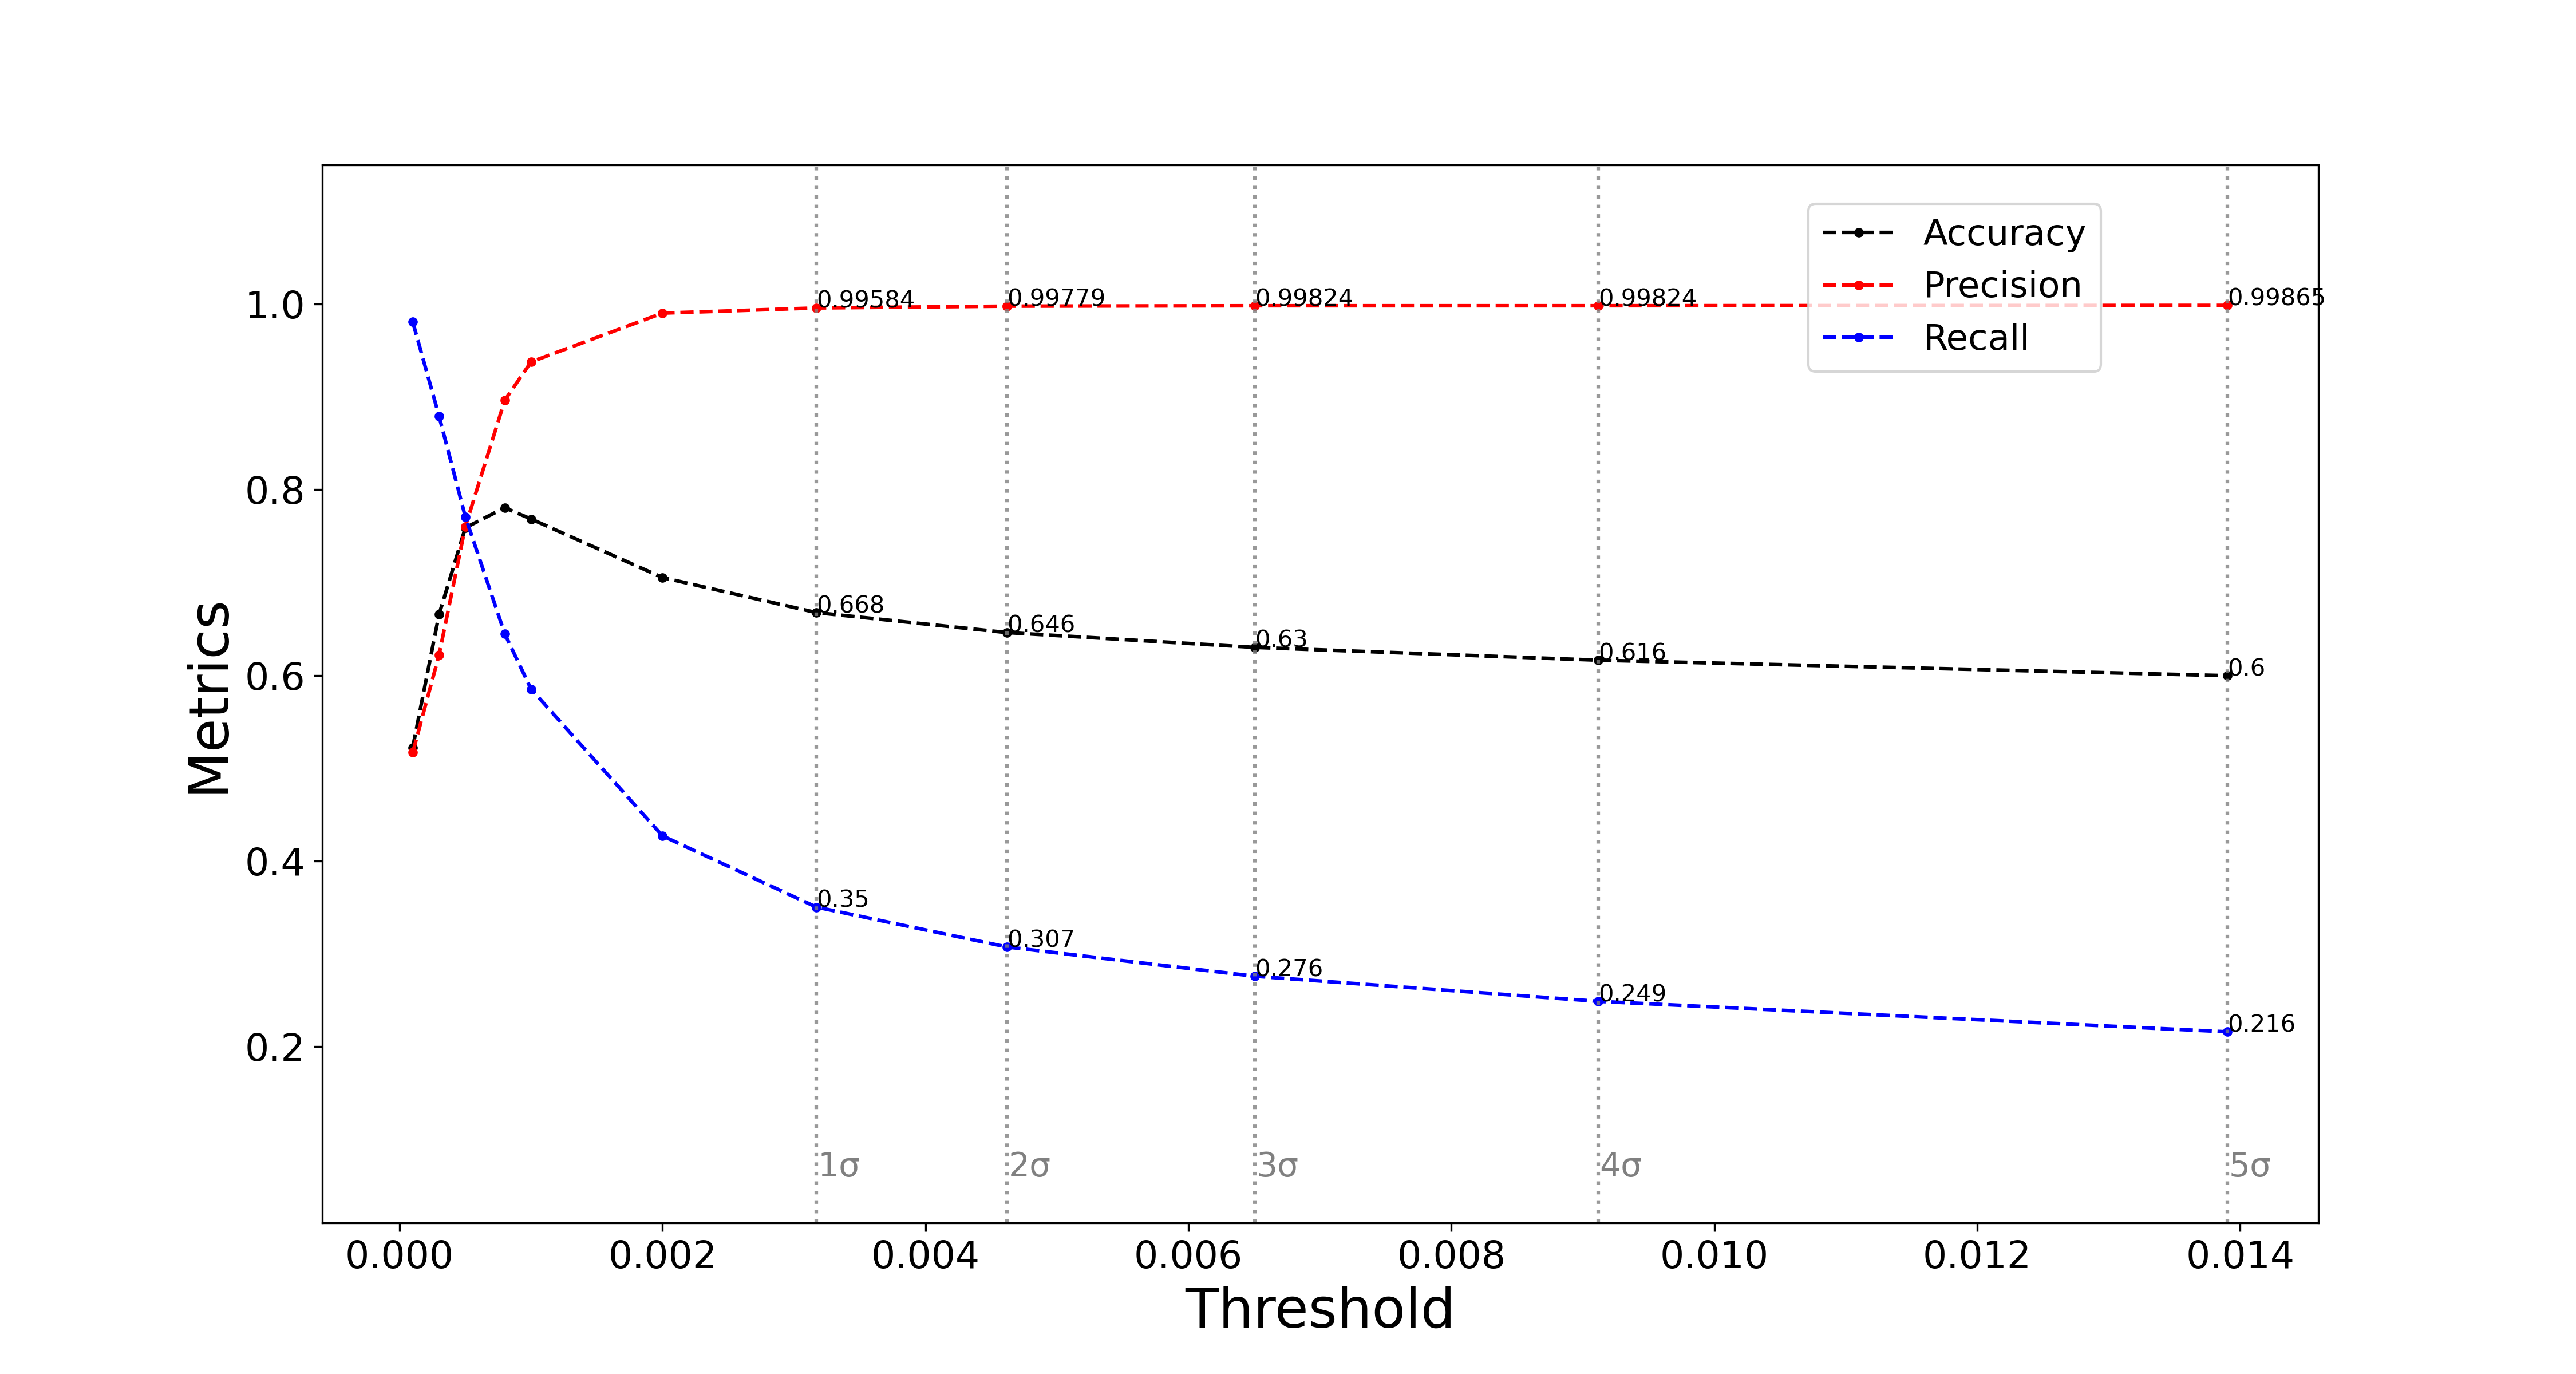
\includegraphics[width=\linewidth]{figures/experiments/metrics/cnn_metrics_test_set_all_itime_5.png}
    \caption{Accuracy, precision and recall curves for the Anomaly Detector with CNN layers in the short term settings (integration time = 5).}
    \label{fig:cnn-metrics-itime-5-appendix}
\end{figure}

\begin{figure}[!htb]
    \centering
    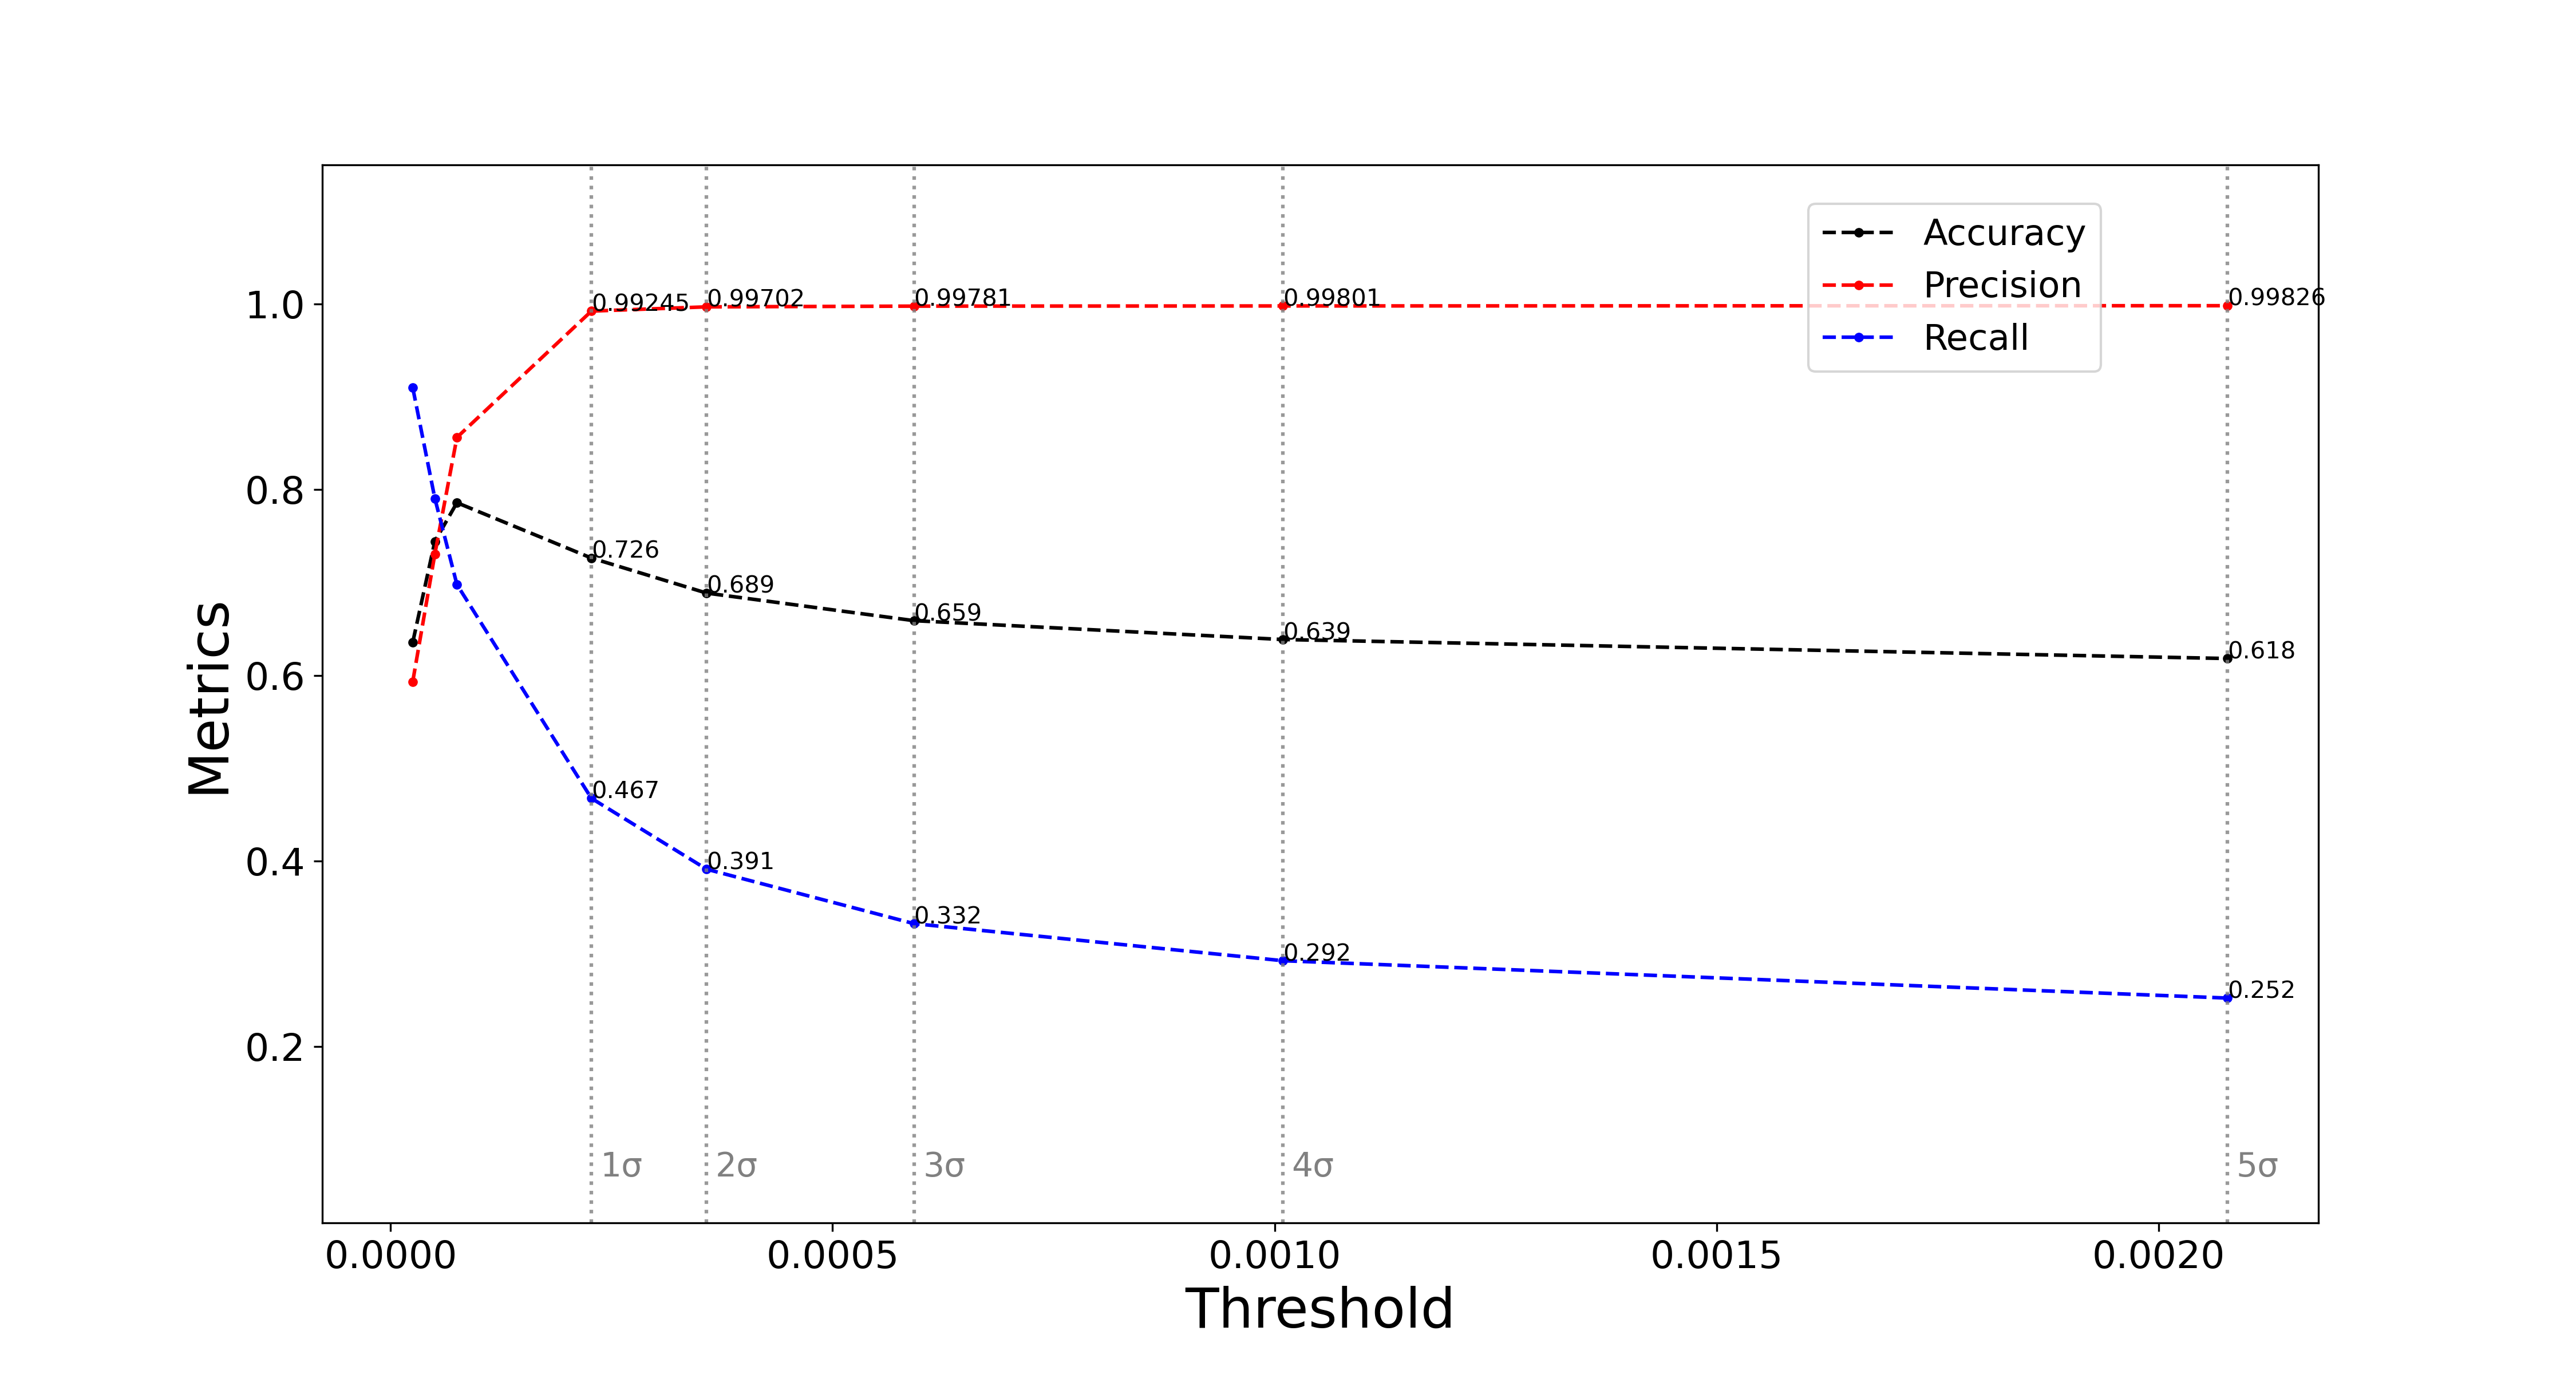
\includegraphics[width=\linewidth]{figures/experiments/metrics/rnn_metrics_test_set_all_itime_5.png}
    \caption{Accuracy, precision and recall curves for the Anomaly Detector with RNN layers in the short term settings (integration time = 5).}
    \label{fig:rnn-metrics-itime-5-appendix}
\end{figure}

\begin{figure}[!htb]
    \centering
    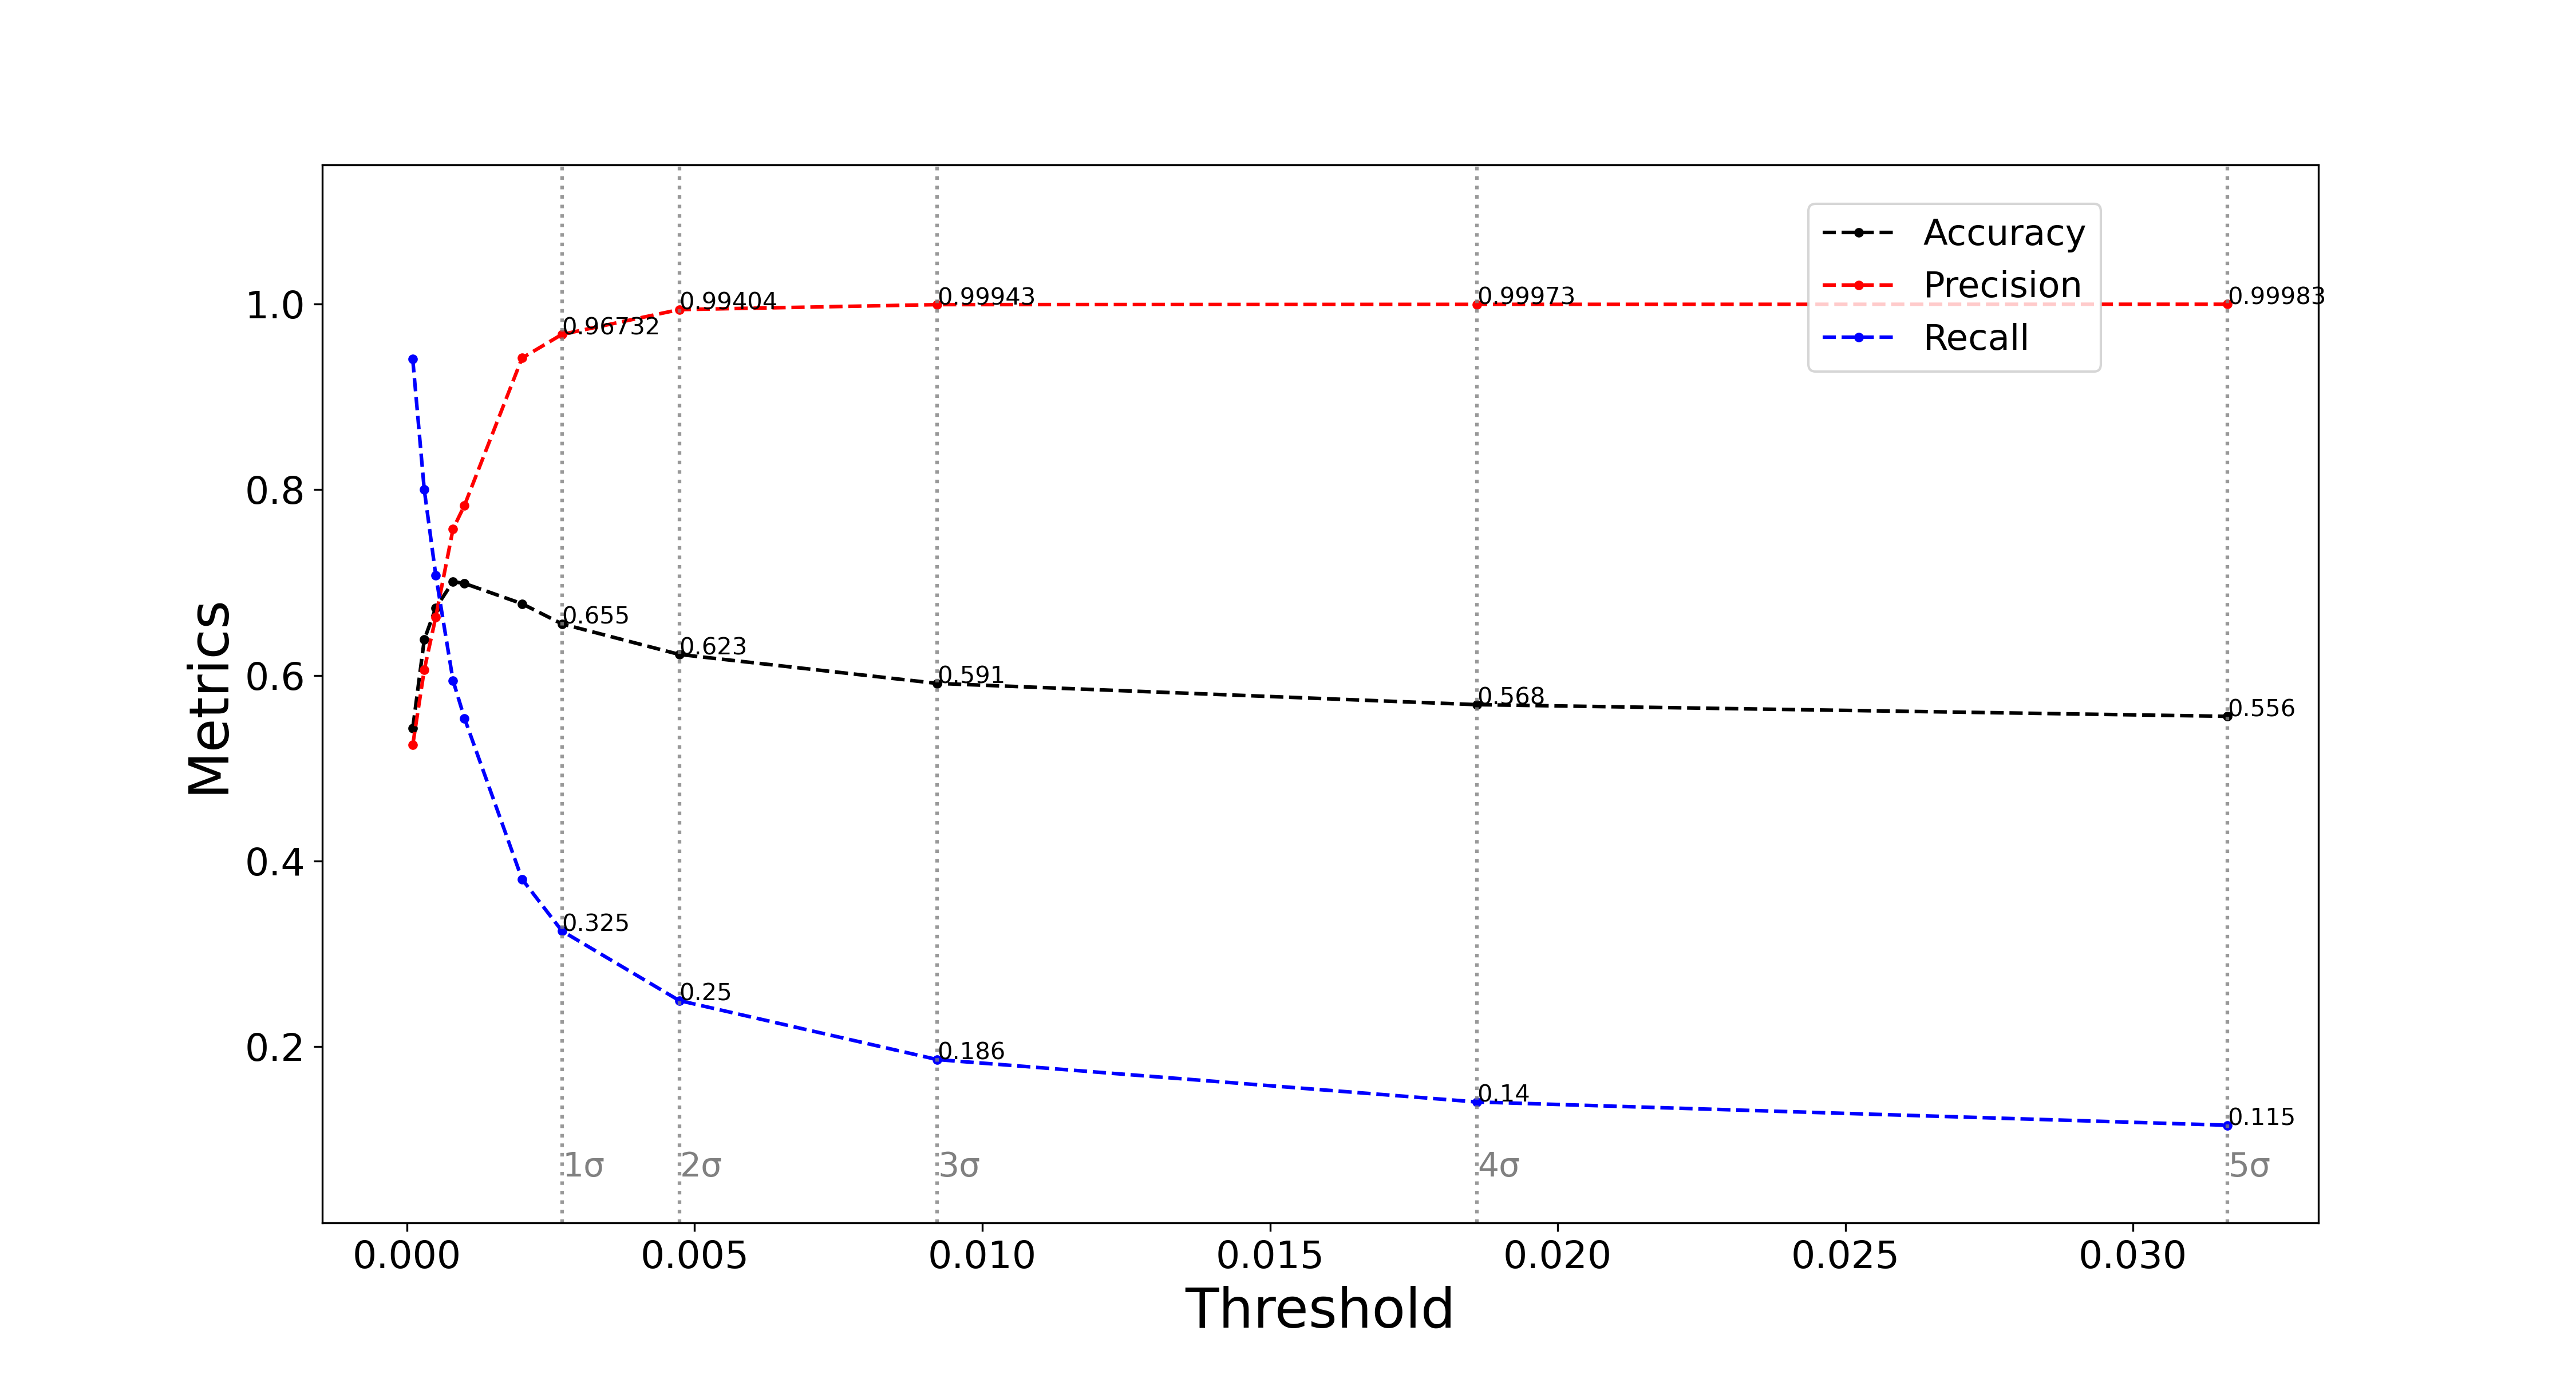
\includegraphics[width=\linewidth]{figures/experiments/metrics/cnn_metrics_test_set_all_itime_1.png}
    \caption{Accuracy, precision and recall curves for the Anomaly Detector with CNN layers in the very short term settings (integration time = 1).}
    \label{fig:cnn-metrics-itime-1-appendix}
\end{figure}

\begin{figure}[!htb]
    \centering
    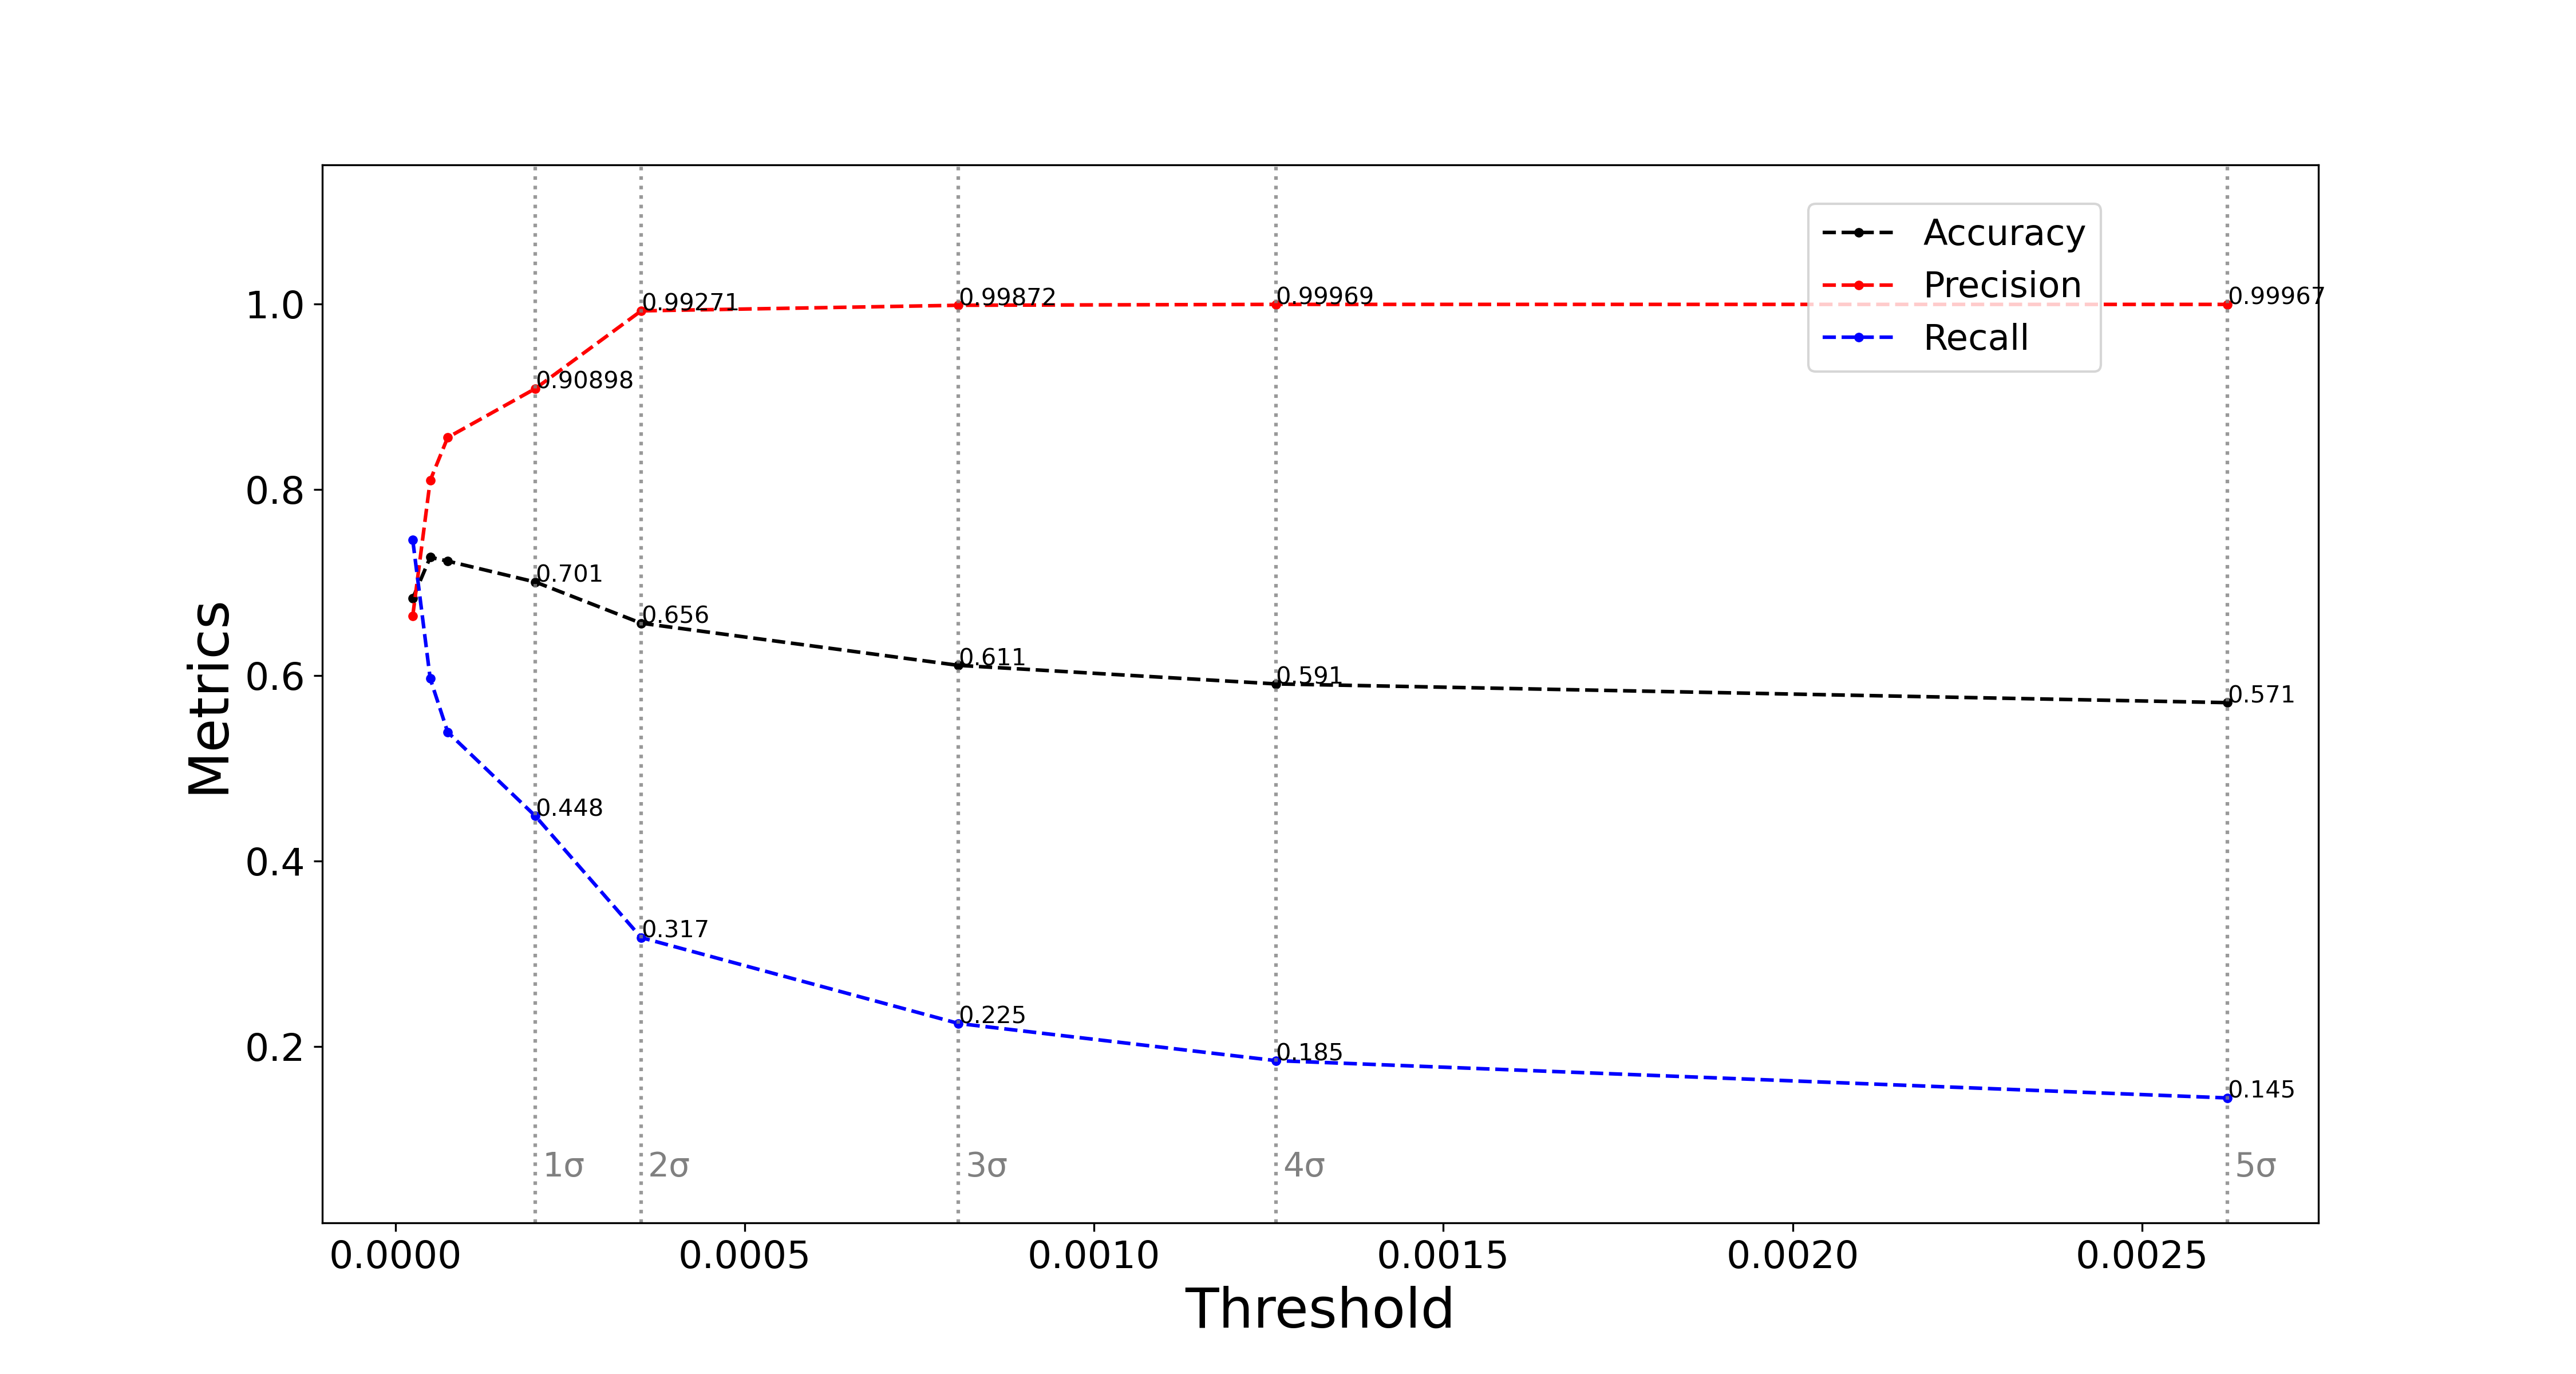
\includegraphics[width=\linewidth]{figures/experiments/metrics/rnn_metrics_test_set_all_itime_1.png}
    \caption{Accuracy, precision and recall curves for the Anomaly Detector with RNN layers in the short term settings (integration time = 1).}
    \label{fig:rnn-metrics-itime-1-appendix}
\end{figure}




\FloatBarrier
\section{}
  \newpage

  \chapter{Appendix C}\label{c:AppendixC}
  
%%%%%%%%%%%%%%%%%%%%%%%%%%%%%%%%%%%%%%%%%%%%%%%%%%%%%%%%%%%%%%%%%%%%%%%%%%%%%
\section{Results}
\label{s:appendix-c}


\begin{figure}[!htb]
    
    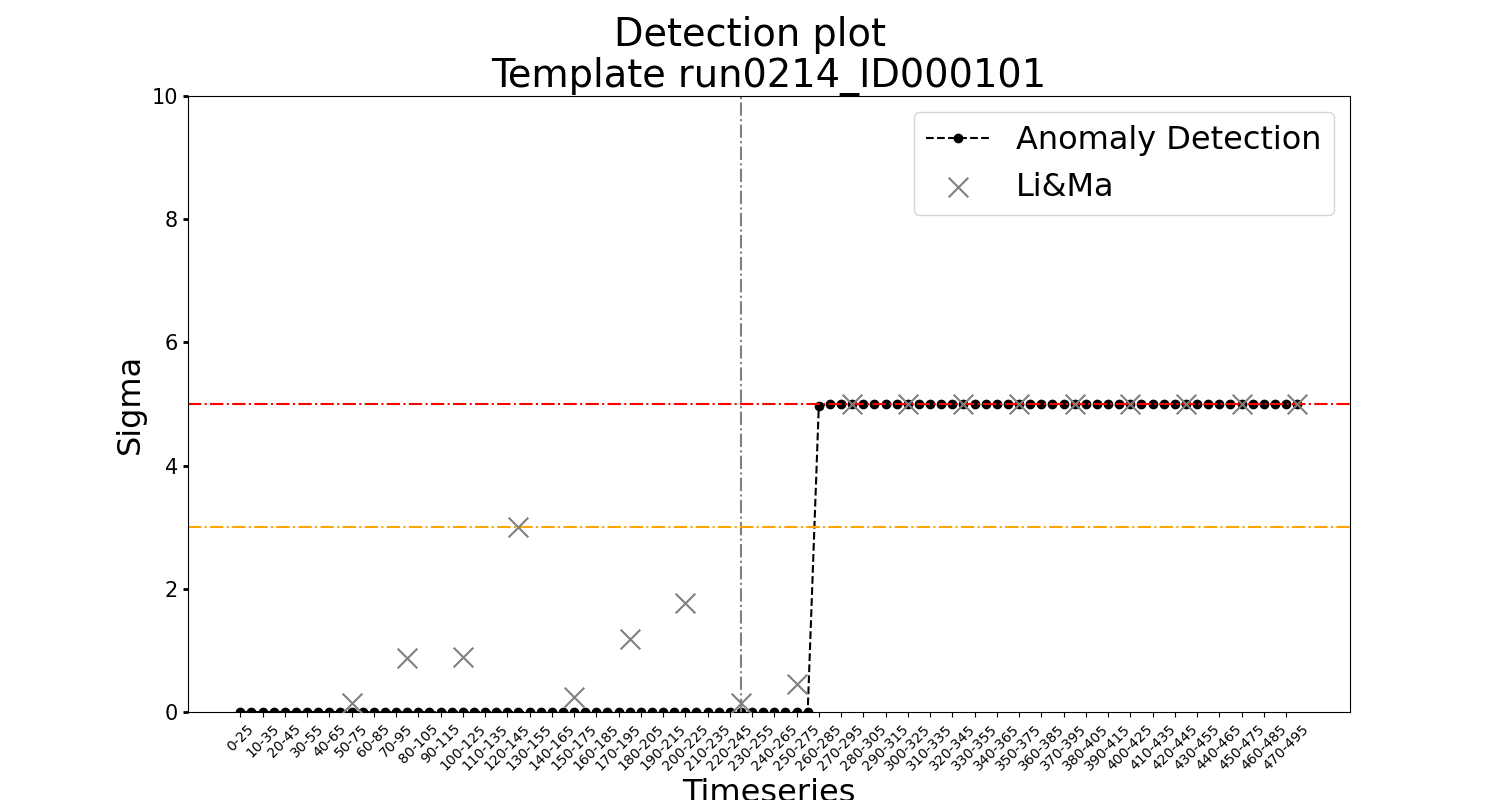
\includegraphics[width=1\textwidth]{figures/experiments/detection_plots/detection_plot_run0214_ID000101_testset_e.png}\hfill
    \\[\smallskipamount]
    
    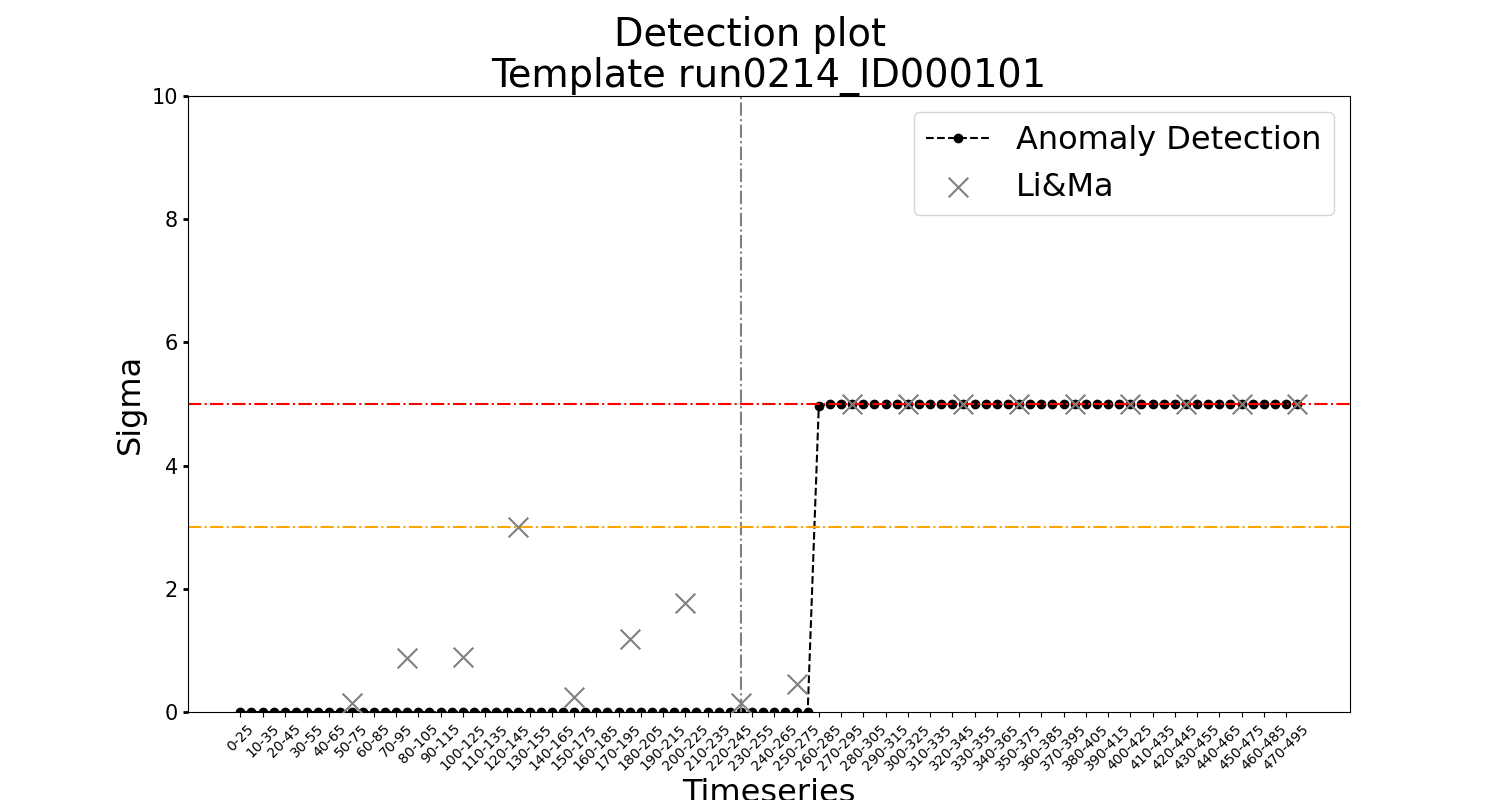
\includegraphics[width=1\textwidth]{figures/experiments/detection_plots/detection_plot_run0214_ID000101_testset_e.png}\hfill
    \\[\smallskipamount]

    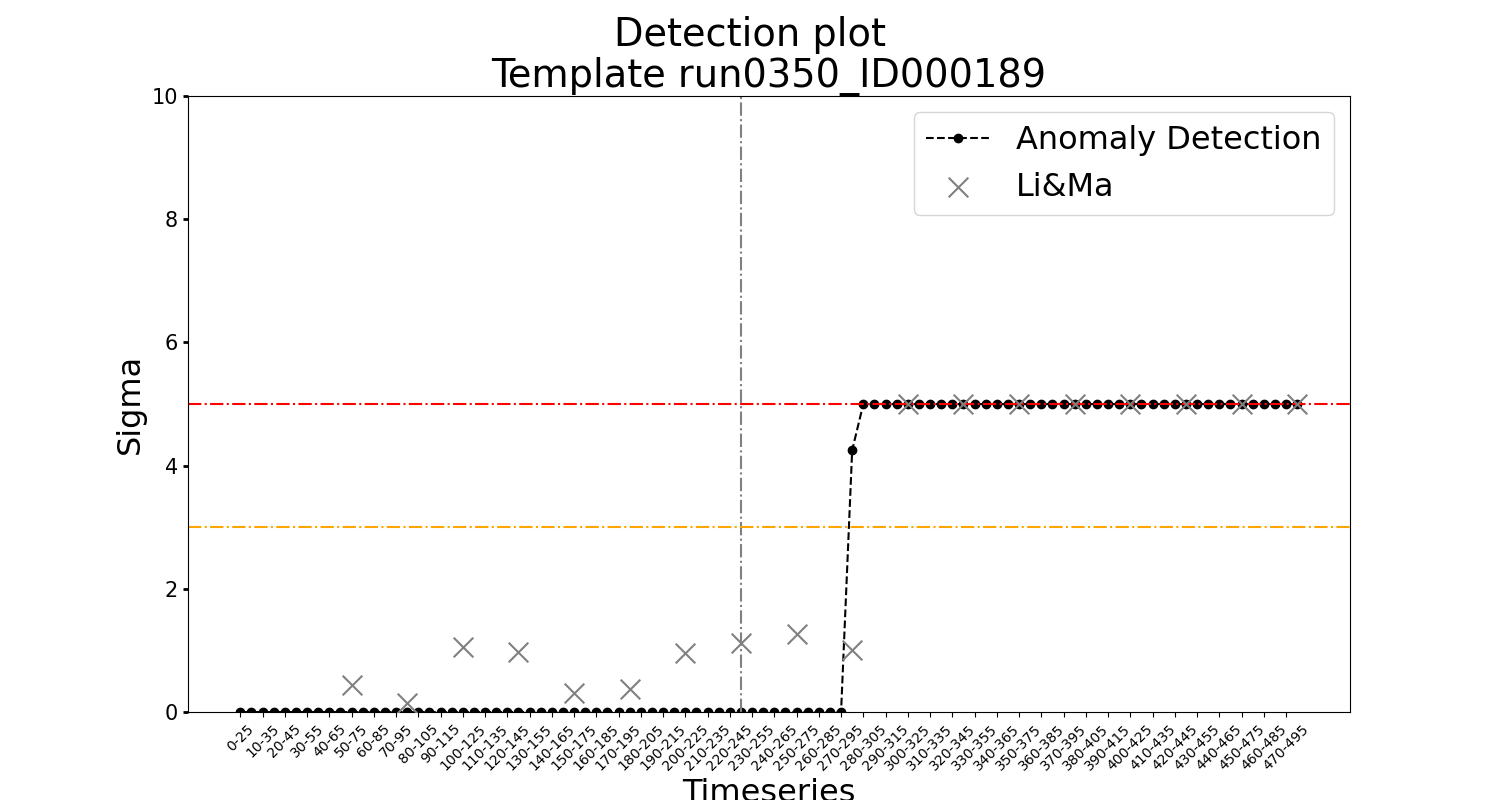
\includegraphics[width=1\textwidth]{figures/experiments/detection_plots/detection_plot_run0350_ID000189_testset_e.png}\hfill
    \\[\smallskipamount]

    \caption{Detection plots 1}\label{fig:detection-plots-1}
\end{figure}


\begin{figure}[!htb]
    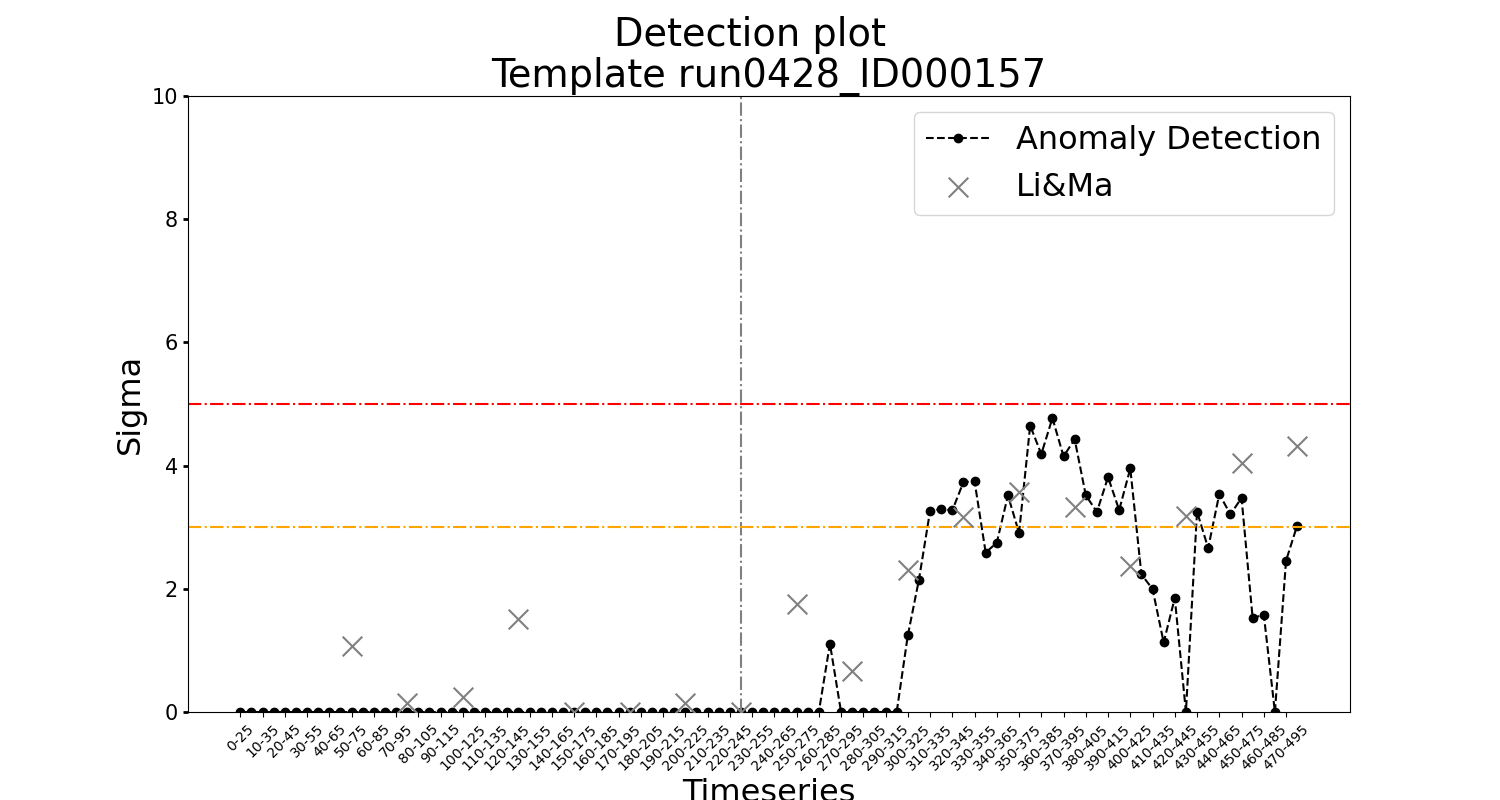
\includegraphics[width=1\textwidth]{figures/experiments/detection_plots/detection_plot_run0428_ID000157_testset_e.png}\hfill
    \\[\smallskipamount]

    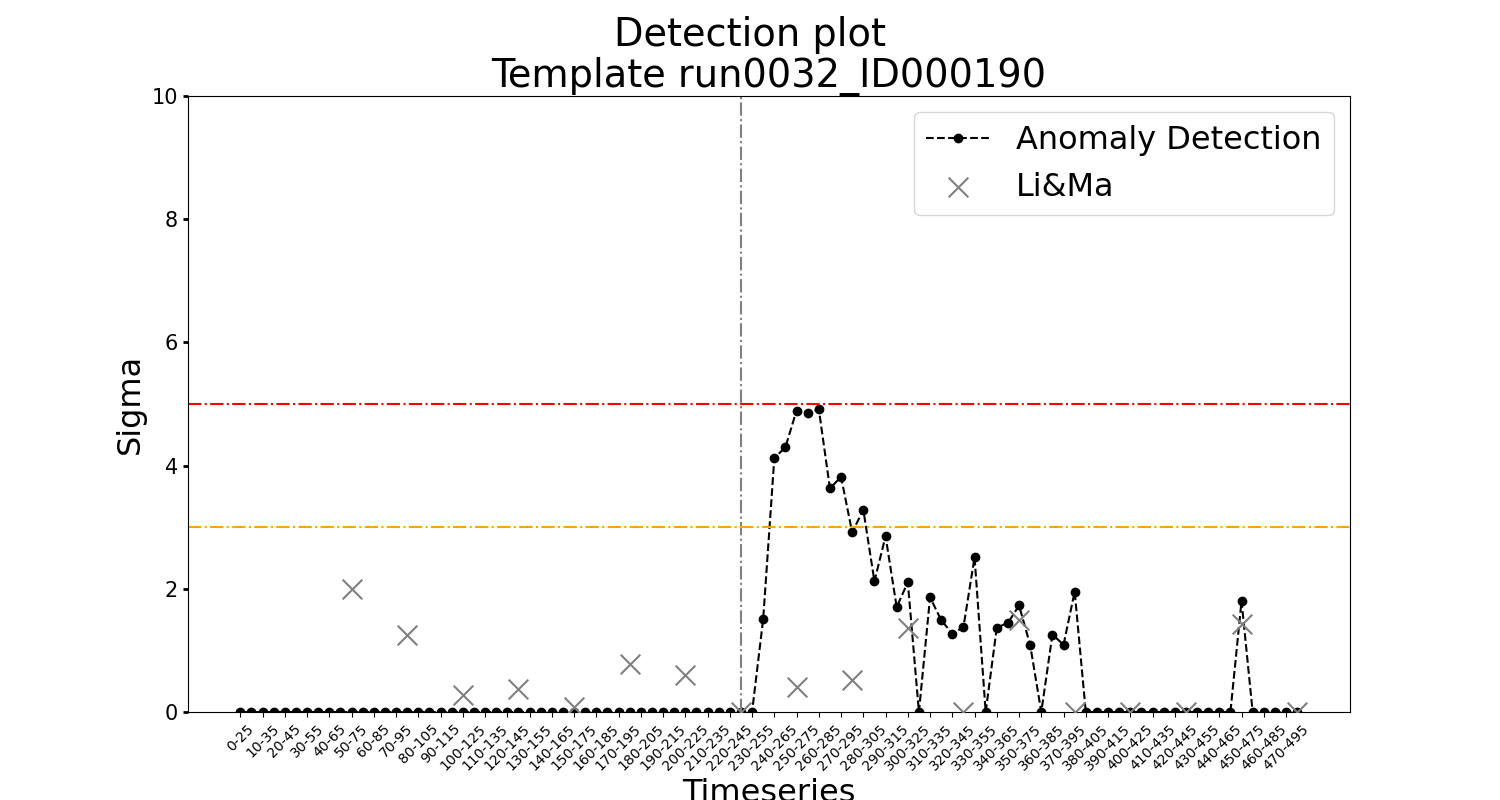
\includegraphics[width=1\textwidth]{figures/experiments/detection_plots/detection_plot_run0032_ID000190_testset_e.png}\hfill
    \\[\smallskipamount]
    
    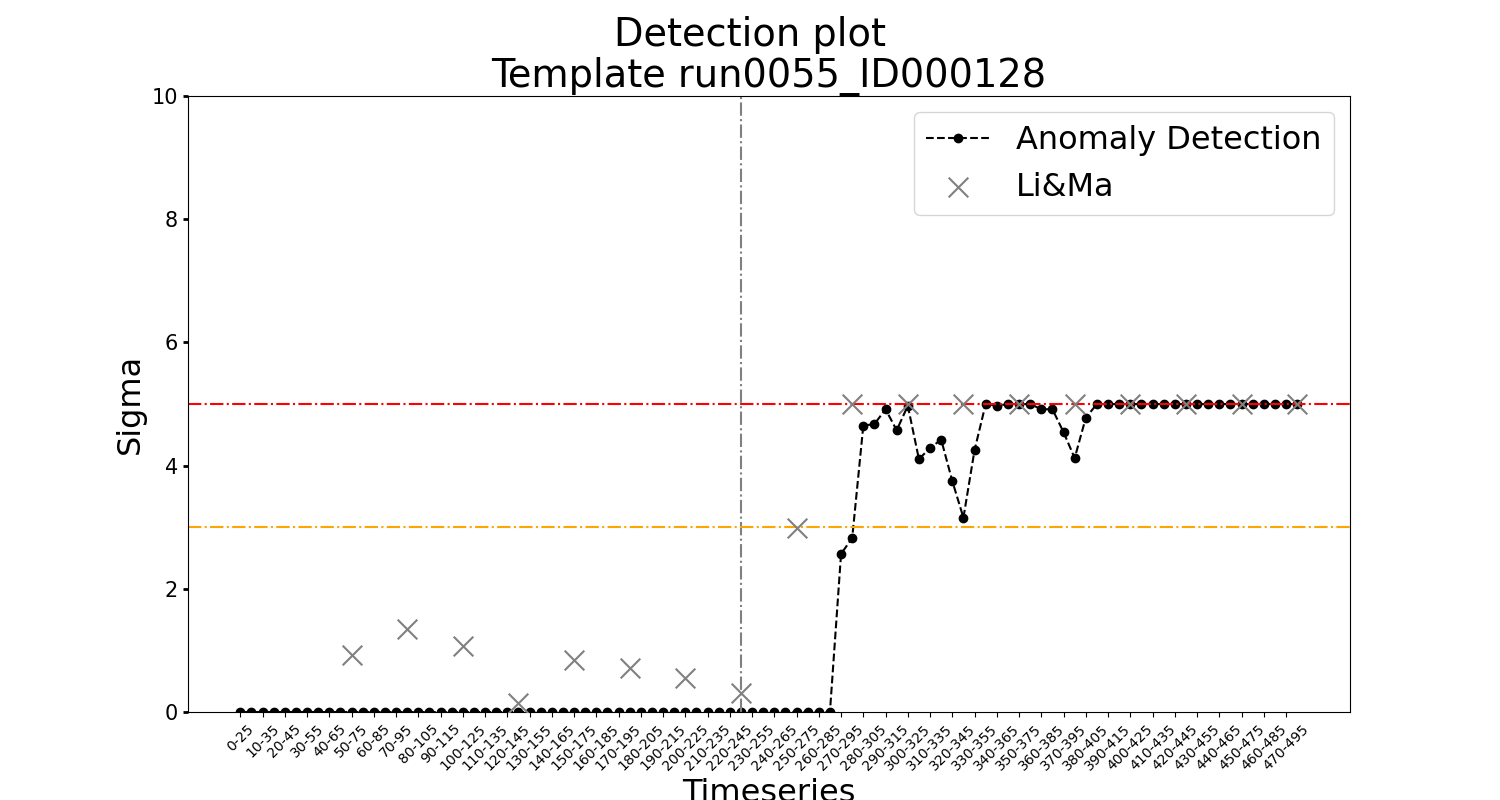
\includegraphics[width=1\textwidth]{figures/experiments/detection_plots/detection_plot_run0055_ID000128_testset_e.png}\hfill
    \\[\smallskipamount]
    \caption{Detection plots 2}\label{fig:detection-plots-2}
\end{figure}



\begin{figure}[!htb]
    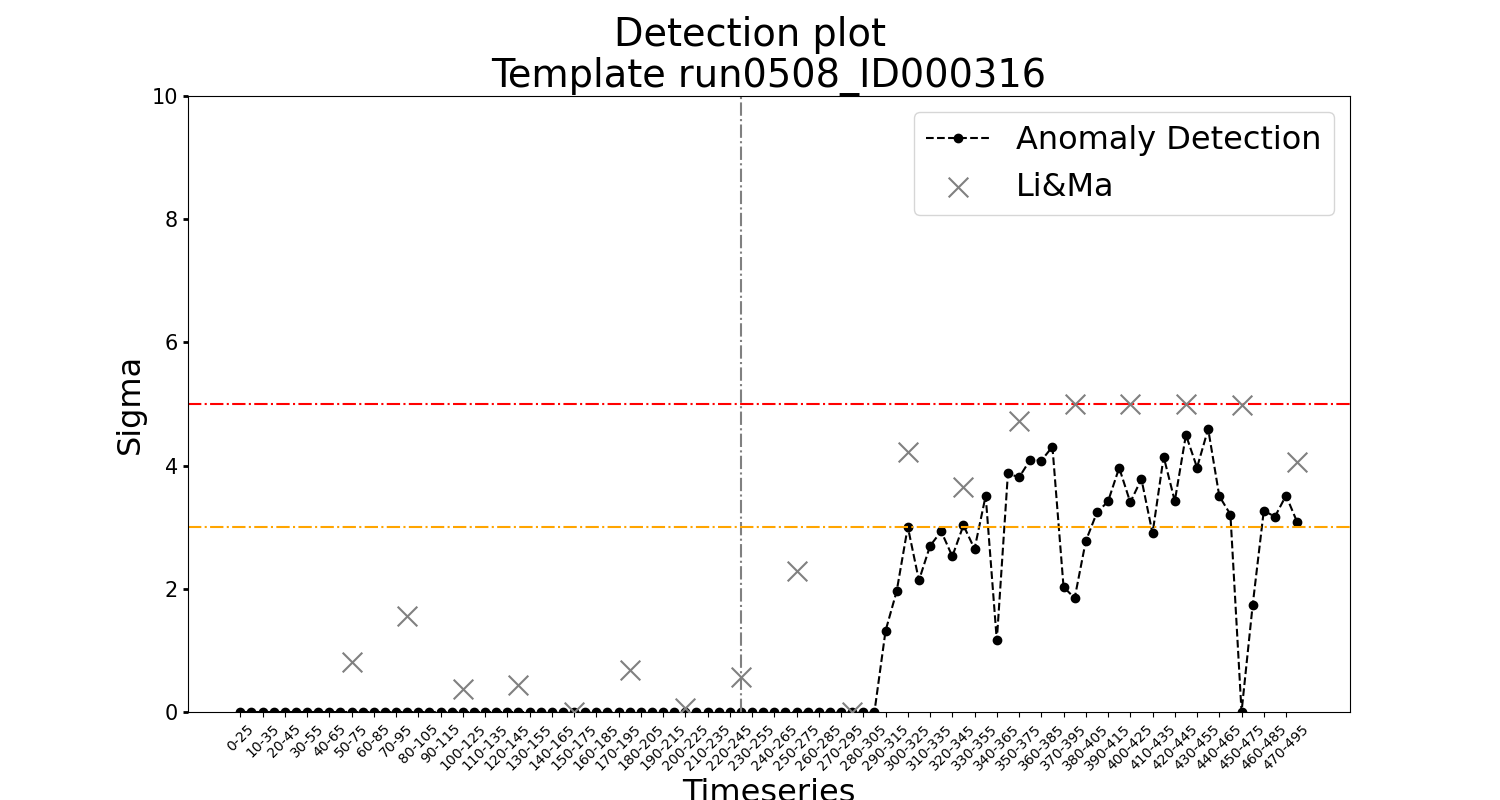
\includegraphics[width=1\textwidth]{figures/experiments/detection_plots/detection_plot_run0508_ID000316_testset_e.png}\hfill
    \\[\smallskipamount]

    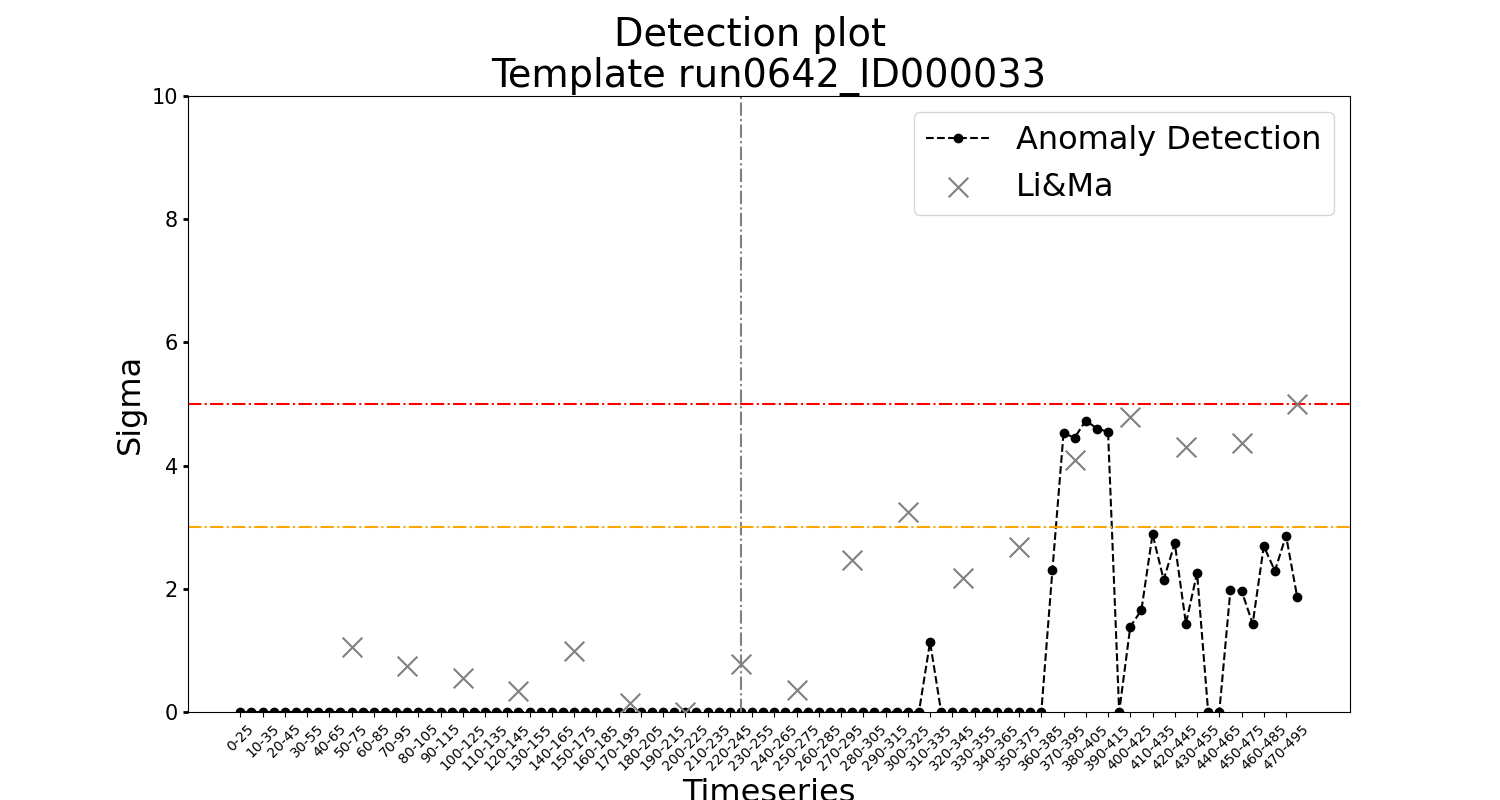
\includegraphics[width=1\textwidth]{figures/experiments/detection_plots/detection_plot_run0642_ID000033_testset_e.png}\hfill
    \\[\smallskipamount]
    
    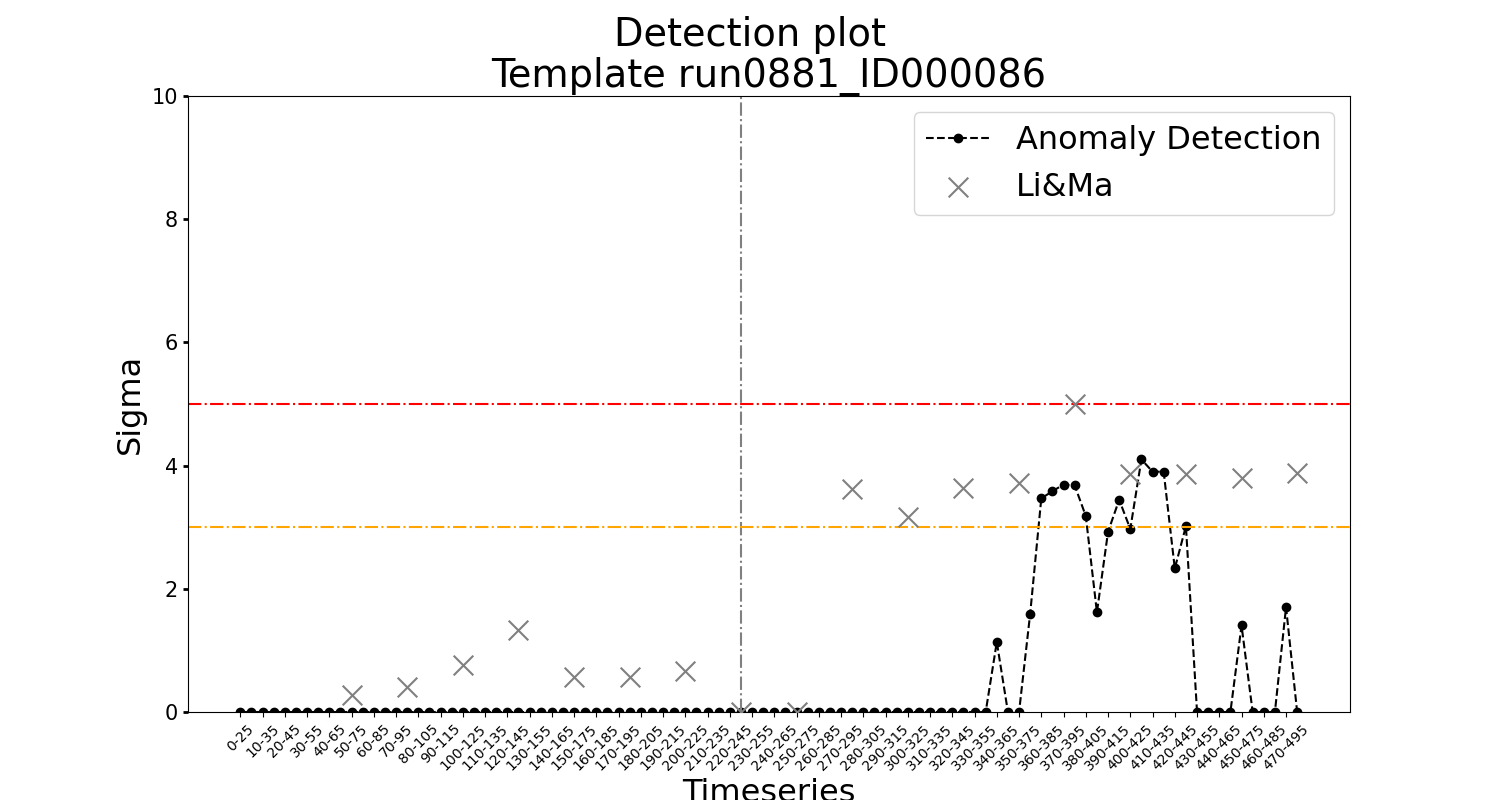
\includegraphics[width=1\textwidth]{figures/experiments/detection_plots/detection_plot_run0881_ID000086_testset_e.png}\hfill
    \\[\smallskipamount]
    \caption{Detection plots 2}\label{fig:detection-plots-2}
\end{figure}
\FloatBarrier
\section{}
  \newpage

  
  \cleardoublepage
  \appendix

  
  \singlespacing
  % Bibliography
\label{app:Bibliography} % Reference the bibliography elsewhere with \autoref{app:Bibliography}

\manualmark % Work-around to have small caps also here in the headline
\markboth{\spacedlowsmallcaps{\bibname}}{\spacedlowsmallcaps{\bibname}} % Work-around to have small caps also
%\phantomsection
\refstepcounter{dummy}

\addtocontents{toc}{\protect\vspace{\beforebibskip}} % Place the bibliography slightly below the rest of the document content in the table of contents
\addcontentsline{toc}{chapter}{\tocEntry{\bibname}}
\printbibliography
  \cleardoublepage

  \newpage
  \chapter*{Publications}
\addcontentsline{toc}{chapter}{Publications}

\hinttext{This page is mandatory. The content and structure must comply with the regulations of your school or department. Rules and regulations may change during your candidature. Please consult the \emph{guidelines for preparing a thesis}\footnote{\url{https://www.latrobe.edu.au/researchers/grs/hdr/candidature/forms-and-resources}} to make sure you got things right. Talk with your supervisor or research coordinator if you intend to deviate from the standard.}

This thesis includes work by the author that has been published or accepted for publication. These publications are the own work of the author of this thesis, and the author has the permission of the publishers to reproduce the contents of these publications for academic purposes.

In particular, some data, ideas, opinions and figures presented in this thesis have previously appeared or may appear shortly after the submission of this thesis as follows:
\begin{itemize}

  \item \hinttext{You MUST list all you publications that are quoted verbatim throughout your thesis here! Make sure this is complete to protect yourself from the accusation of academic misconduct. Self-plagiarism is also plagiarism! Make sure that you have the permission of the respective journals and your co-authors if you intend to quote passages from papers verbatim.}
  
  \item Feyd-Rautha Harkonnen, Glossu Rabban ``\textbf{How to use Ixian Probes to Extract Memories from Tleilaxu Masters}'' accepted for publication in \emph{Technological and Scientific Journal of the Spacing Guild}, ISSN: 1234-5678, DOI: \href{https://en.wikipedia.org/wiki/Spacing_Guild}{99.8765/SPACE.2018.312134}
  
  \item Feyd-Rautha Harkonnen, Shaddam Corrino, Piter De Vries ``\textbf{A novel approach to use the Holtzmann Effect to break through shield walls}'' published in \emph{League Worlds Joint Engineering Society Journal}, ISSN: 9122-9122, DOI: \href{https://en.wikipedia.org/wiki/Organizations_of_the_Dune_universe#Landsraad}{00.1234/LRAAD.2018.123344}
  
  \item Piter De Vries, Feyd-Rautha Harkonnen ``\textbf{Why the Spice must flow?}'' \textendash{} Working draft currently under preparation for submission. \hinttext{This is not required, but it may be useful in case your thesis is accepted earlier than your paper.}
  
\end{itemize}
Except where reference is made in the text of the thesis, this thesis contains no other material published elsewhere or extracted in whole or in part from a thesis accepted for the award of any other degree or diploma. No other person's work has been used without due acknowledgment in the main text of the thesis. This thesis has not been submitted for the award of any degree or diploma in any other tertiary institution.


  
  \pagestyle{empty}
  \onehalfspacing
  
\end{document}